%%%%%%%%%%%%%%%%%%%%%%%%%%%%%%%%%%%%%%%%%
% Memoria para Trabajos Final es de la 
% Carrera de Especialización en 
% Sistemas Embebidos de la FIUBA
%
% Versión 3.00 (11/10/2016)
%
% Basado en:

% Masters/Doctoral Thesis 
% LaTeX Template
% Version 2.3 (25/3/16)
%
% Version 2.x major modifications by:
% Vel (vel@latextemplates.com)
%
% This template is based on a template by:
% Steve Gunn (http://users.ecs.soton.ac.uk/srg/softwaretools/document/templates/)
% Sunil Patel (http://www.sunilpatel.co.uk/thesis-template/)
%
% Template license:
% CC BY-NC-SA 3.0 (http://creativecommons.org/licenses/by-nc-sa/3.0/)
%
%%%%%%%%%%%%%%%%%%%%%%%%%%%%%%%%%%%%%%%%%

%----------------------------------------------------------------------------------------
%	PACKAGES AND OTHER DOCUMENT CONFIGURATIONS
%----------------------------------------------------------------------------------------

\documentclass[
11pt, % The default document font size, options: 10pt, 11pt, 12pt
%oneside, % Two side (alternating margins) for binding by default, uncomment to switch to one side
%chapterinoneline,% Have the chapter title next to the number in one single line
%english, % ngerman for German
spanish,
singlespacing, % Single line spacing, alternatives: onehalfspacing or doublespacing
%draft, % Uncomment to enable draft mode (no pictures, no links, overfull hboxes indicated)
%nolistspacing, % If the document is onehalfspacing or doublespacing, uncomment this to set spacing in lists to single
%liststotoc, % Uncomment to add the list of figures/tables/etc to the table of contents
%toctotoc, % Uncomment to add the main table of contents to the table of contents
parskip, % Uncomment to add space between paragraphs
%nohyperref, % Uncomment to not load the hyperref package
headsepline, % Uncomment to get a line under the header
]{MastersDoctoralThesis} % The class file specifying the document structure



\usepackage[utf8]{inputenc} % Required for inputting international characters
\usepackage[T1]{fontenc} % Output font encoding for international characters

\usepackage{palatino} % Use the Palatino font by default
\usepackage[backend=bibtex,natbib=true]{biblatex} % Use the bibtex backend

\addbibresource{references.bib} % The filename of the bibliography

\usepackage[autostyle=true]{csquotes} % Required to generate language-dependent quotes in the bibliography

\usepackage{caption}
\usepackage{subcaption}

%------------------------
\usepackage{listings}

%\usepackage[hyphens]{url}
%\usepackage[hidelinks]{hyperref}
%\hypersetup{breaklinks=true}
%\urlstyle{same}
%\usepackage{cite}

%--------------------------

\usepackage{color}
\usepackage{graphicx}
\usepackage{float}
\usepackage{wrapfig}
%\usepackage{subfig}
%\usepackage{subcaption}
% \usepackage{mathabx}
% \usepackage{amsfonts}
\usepackage{amsmath}
\usepackage{amssymb}
% \usepackage{amsthm}
% \usepackage{mathrsfs}
% \usepackage{float}

%
%----------------------------------------------------------------------------------------
%	MARGIN SETTINGS
%----------------------------------------------------------------------------------------

\geometry{
	paper=a4paper, % Change to letterpaper for US letter
	inner=2cm, % Inner margin
	outer=3.3cm, % Outer margin
	bindingoffset=2cm, % Binding offset
	top=1.5cm, % Top margin
	bottom=1.5cm, % Bottom margin
	%showframe,% show how the type block is set on the page
}

%----------------------------------------------------------------------------------------
%	INFORMACIÓN DE LA PORTADA
%----------------------------------------------------------------------------------------

\thesistitle{Implementación y análisis de algoritmos de cálculo de Transformada Rápida de
	Fourier para su aplicación en sistemas OFDM} % El títulos de la memoria, se usa en la carátula y se puede usar el cualquier lugar del documento con el comando \ttitle
\supervisor{Dr. Ing. Ariel Lutenberg} % El nombre del director, se usa en la carátula y se puede
% usar el cualquier lugar del documento con el comando \supname
\cosupervisor{Ing. Fedeerico Giordano Zacchigna}
\degree{Ingeniero Electrónico} % Nombre del grado, se usa en la carátula y se puede usar el
% cualquier lugar del documento con el comando \degreename
\author{Andrés Dario Cassagnes} % Tu nombre, se usa en la carátula y se puede usar el cualquier
% lugar del documento con el comando \authorname
\juradoUNO{Dr. Ing. Leonardo Rey Vega} % Nombre y pertenencia del un jurado se usa en la carátula y
% se puede usar el cualquier lugar del documento con el comando \jur1name
\juradoDOS{Ing. Carlos Belaustegui Goitia} % Nombre y pertenencia del un jurado se usa en la
% carátula y se puede usar el cualquier lugar del documento con el comando \jur2name
\juradoTRES{Ing. Nicolas Álvarez} % Nombre y pertenencia del un jurado se usa en la carátula y se
% puede usar el cualquier lugar del documento con el comando \jur3name
\fechaINICIO{enero de 2016}
\fechaFINAL{diciembre de 2016}

%----------------------------------------------------------------------------------------
%	FIN INFORMACIÓN DE LA PORTADA
%----------------------------------------------------------------------------------------

\subject{Memoria del Trabajo de Tesis de la Carrera de Ingeniería en Electrónica de la
UBA}
% Your subject area, this is not currently used anywhere in the template, print it elsewhere with \subjectname
\keywords{OFDM, FFT, Sistemas Digitales, FPGA} % Keywords for your thesis, this is not currently
% used anywhere in the template, print it elsewhere with \keywordnames
\university{Universidad de Buenos Aires} % Your university's name and URL, this is used in the title page and abstract, print it elsewhere with \univname
\faculty{{Facultad de Ingeniería}} % Your faculty's name and URL, this is used in the title page and abstract, print it elsewhere with \facname
\department{Departamento de Electrónica} % Your department's name and URL, this is used in the title page and abstract, print it elsewhere with \deptname
\group{{Laboratorio de Sistemas Embebidos}} % Your research group's name and URL, this is used in the title page, print it elsewhere with \groupname


\hypersetup{pdftitle=\ttitle} % Set the PDF's title to your title
\hypersetup{pdfauthor=\authorname} % Set the PDF's author to your name
\hypersetup{pdfkeywords=\keywordnames} % Set the PDF's keywords to your keywords


\newcaptionname{spanish}{\acknowledgementname}{Agradecimientos}
\newcaptionname{spanish}{\authorshipname}{Declaración de Autoría}
\newcaptionname{spanish}{\abbrevname}{Glosario}
\newcaptionname{spanish}{\byname}{por}

\renewcommand{\lstlistingname}{Algoritmo}% Listing -> Algorithm
\renewcommand{\lstlistlistingname}{Índice de \lstlistingname s}% List of Listings -> List of Algorithms

\renewcommand{\listtablename}{Índice de Tablas}
\renewcommand{\tablename}{Tabla} 

\addtolength{\footnotesep}{2mm} % Espacio adicional en los footnotes

\begin{document}

\frontmatter % Use roman page numbering style (i, ii, iii, iv...) for the pre-content pages

\pagestyle{plain} % Default to the plain heading style until the thesis style is called for the body content

%----------------------------------------------------------------------------------------
%	PORTADA
%----------------------------------------------------------------------------------------

\begin{titlepage}
\begin{center}

{\scshape\LARGE UNIVERSIDAD DE BUENOS AIRES\par}\vspace{0.1cm} % University name
{\scshape\LARGE FACULTAD DE INGENIERÍA\par}\vspace{0.1cm} % Faculty name
{\scshape\LARGE Ingeniería en Electrónica\par}\vspace{1cm} % Thesis type


\includegraphics[width=.3\textwidth]{./figures/logoFIUBA.png}
\vspace{1cm}

\textsc{\Large Memoria del Trabajo de Tesis}\\[0.5cm] % Thesis type

{\huge \bfseries \ttitle\par}\vspace{0.4cm} % Thesis title

\vspace{1cm}
\LARGE\textbf{Autor:\\
\authorname}\\ % Author name

%\vspace{1cm}

\large
\vspace{10px}
{Director:} \\
{\supname} % Supervisor name

\large
\vspace{10px}
{Codirector:} \\
{\cosupname} % Supervisor name

\vspace{10px} 
%\vspace{1cm}
Jurados:\\
\jurunoname\\
\jurdosname\\
\jurtresname
 
\vfill
\textit{Este trabajo fue realizado en la ciudad de San Carlos de Bariloche y en la Ciudad Autónoma
de Buenos Aires, entre
\fechaINICIOname
\hspace{1px} y \fechaFINALname.}
\end{center}
\end{titlepage}


%----------------------------------------------------------------------------------------
%	RESUMEN
%----------------------------------------------------------------------------------------

\begin{abstract}
\addchaptertocentry{\abstractname} % Add the abstract to the table of contents
%
%The Thesis Abstract is written here (and usually kept to just this page). The page is kept centered vertically so can expand into the blank space above the title too\ldots
\centering

El objetivo de este trabajo es el diseño y la implementación en hardware digital de una arquitectura
de cómputo de la transformada rápida de Fourier para ser utilizada en la modulación y demodulación
de un sistema de comunicaciones OFDM. El trabajo de tesis se encuadra dentro del proyecto Software
Defined Radio del Laboratorio de Sistemas Embebidos.

Se presenta la teoría de base necesaria para poder explicar los desarrollos realizados. Se
realiza una introducción teórica a la transformada rápida de Fourier y su utilización en los
sistemas de comunicación OFDM, realizando una breve reseña de la teoría de estos sistemas de
comunicación.

Se describen las arquitecturas desarrolladas durante el trabajo de tesis, explicando en cada caso
el criterio utilizado para la selección de las arquitecturas y algoritmos a implementar. 

Por último, se analizan los resultados obtenidos, determinando la utilidad de la o las
arquitecturas implementadas para el fin para el cual se desarrollaron en base a ese análisis, y se
proponen trabajos futuros.

\end{abstract}

%----------------------------------------------------------------------------------------
%	AGRADECIMIENTOS
%----------------------------------------------------------------------------------------

\begin{acknowledgements}
%\addchaptertocentry{\acknowledgementname} % Descomentando esta línea se puede agregar los agradecimientos al índice
\vspace{1.5cm}

En primer lugar quiero agradecerle a mi director de tesis, el Dr. Ing. Ariel Lutenberg, mi
co-director, el Ing. Federico Gioradno Zacchigna, apodado afectuosamente como el ''Colo'', y al Ing.
Octavio Alpago, por haberme guíado, ayudado y aconsejado durante el desarrollo del trabajo de
tesis. También quiero agradecerles por permitirme ser parte del proyecto Software Define Radio en
el cual se enmarca el presente trabajo.

Agradezco especialmente a los miembros del jurado, el Dr. Ing. Leonardo Rey Vega, el Ing. Carlos
Belaustegui Goitia y el Ing. Nicolás Alvarez por dedicar tiempo a la evaluación de este trabajo.

Quiero agradecer muy especialmente a mi esposa, Analía, por apoyarme, acompañarme, soportarme,
incentivarme, y a veces marcarme el camino con cierta firmeza, a lo largo de la carrera y la
realización del presente trabajo de tesis. Su apoyo y paciencia fueron fundamentales para la
finalización de esta etapa de mi vida.

A mis padres, grandes responsables de la persona que soy, y de quienes aprendí el valor de la
perseverancia y el trabajo duro. A mi hermano Luis y su familia, Adriana y Agustín, por aceptarme
en su hogar en los primeros años de la carrera.\\
A la familia Rodas, por aceptarme y hacerme sentir desde el principio como uno más de la familia.

A mis compañeros de la facultad con quienes desarrollé una amistad más allá de las aulas. Guido
Martinez y Lucho Natale, con quienes cerramos filas en los últimos años de cursada y
encaramos en conjunto el arduo trabajo de la tesis de grado. A Sebastián D'Agostino y Adrián Coria,
con quienes compartí el comienzo de la carrera, cursadas, charlas y una
buena cantidad de cerveza.

A mi amigo de la vida Horacio Arce, apoyo incondicional en todo momento sin importar horas o
distancias.
 
A los compañeros de facultad, a quienes valoro mucho haber conocido y compartido horas, tanto de
cursada como fuera de las aulas. Sebastián Gerez, Juanjo Borges, Juan Pablo Contini, Dario Basso.

A aquellos profesores de quienes me llevo más que solo conceptos de sus materias. Fernando Barreiro,
Carlos Belaustegui, Octavio Alpago, Leandro Santi, Daniel Dalmati, Juan Manuel Cruz. Compartieron no
solo sus conocimientos, sino también su experiencia de vida con total generosidad.

Al Laboratorio de Sistemas Embebidos, y a su director Dr. Ing. Ariel Lutenberg, por abrirme las
puertas, recibirme y brindar un ámbito de trabajo excelente para poder desarrollar no solo el
presente trabajo de tesis sino otros proyectos académicos.

A mis compañeros de trabajo de estos últimos años, el grupo de Instrumentación Neutrónica de INVAP
SE. Darío, Emiliano, Emmanuel, Federico, Fernando y Marcos, por apoyarme, incentivarme, e
inisistirme cuando hizo falta, para que finalice el presente trabajo de tesis.

\end{acknowledgements}

%----------------------------------------------------------------------------------------
%	LISTA DE CONTENIDOS/FIGURAS/TABLAS
%----------------------------------------------------------------------------------------
\renewcommand{\listtablename}{Índice de Tablas}

\tableofcontents % Prints the main table of contents

\listoffigures % Prints the list of figures

\listoftables % Prints the list of tables


%----------------------------------------------------------------------------------------
%	DEDICATORIA
%----------------------------------------------------------------------------------------

\dedicatory{\textbf{A mis padres}}  % escribir acá si se desea una dedicatoria

%----------------------------------------------------------------------------------------
%	CAPÍTULOS
%----------------------------------------------------------------------------------------

\mainmatter % Begin numeric (1,2,3...) page numbering

\pagestyle{thesis} % Return the page headers back to the "thesis" style

\renewcommand{\tablename}{Tabla} 

% Incluir los capítulos como archivos separados desde la carpeta Chapters
% Descomentar las líneas a medida que se escriben los capítulos

\chapter{Introducción al Trabajo de Tesis}

El presente trabajo de tesis se encuentra enfocado en el contexto del diseño de hardware digital. El
mismo fue motivado por el creciente avance en las tecnologías utilizadas en los sistemas de
comunicación en general y en los sistemas \textit{Software Defined
Radio}\footnote{\label{SDR}Software Defined Radio (SDR por sus siglas en inglés): Sistema de
comunicaciones donde los componentes típicamente implementados en hardware (mezcladores, filtros, amplificadores, moduladores / demoduladores, detectores, etc) son
implementados en software.} en particular.
Los sistemas \textit{SDR} permiten implementar sistemas de comunicación mediante software o hardware digital reconfigurable, otorgándoles una gran flexibilidad.\\

La creciente demanda de velocidad en las telecomunicaciones lleva a la implementación de sistemas de
transmisión cada vez más veloces. Uno de los sistemas de transmisión de datos más difundidos es el
sistema \textit{OFDM}, en el cual se utilizan múltiples portadora en las que se modulan los
datos a trasmitir. Una forma práctica y eficiente de implementar las modulación y demodulación
multiportadora requerida por este sistema es mediante el uso de la Transformada Discreta de
Fourier, aprovechando los algoritmos de alta eficiencia disponibles para su implementación.\\

Teniendo en cuenta la complejidad de los sistemas de transmisión \textit{OFDM} y la necesidad de
poder implementarlos en forma eficiente tanto en consumo como en espacio y recursos utilizados, el
presente trabajo de tesis se basa en el desarrollo de un sistema de modulación y demodulación para
transmisiones \textit{OFDM} con muy baja ocupación espacial y de recursos, de manera que pueda ser
integrado fácilmente en sistemas de comunicación reducidos.

\section{Objetivo}
El trabajo de tesis tiene como objetivo diseñar e implementar en hardware digital distintas
arquitecturas capaces de realizar el cálculo de la Transformada Discreta de Fourier (\textit{DFT}
por sus siglas en inglés), teniendo como requerimientos sobre las arquitecturas desarrolladas que
realicen el cálculo en forma eficiente y sean de tamaño reducido. El diseño e implementación será
realizado mediante el lenguaje de modelado de hardware Verilog, orientado a la implementación en
ASIC, mientras que la validación se realizará en un dispositivo FPGA\footnote{\label{FPGA}Field Programmable
Gate Array:
dispositivo semiconductor que contiene bloques de lógica cuya interconexión y funcionalidad
puede ser configurada `in situ' mediante un lenguaje de descripción
especializado.}.\\

El desarrollo de la tesis se divide en una parte teórica y una experimental. Se analizarán distintos
desarrollos algorítmicos para el cálculo de la Transformada Discreta de Fourier, se seleccionarán
los que se consideren más aptos de acuerdo a los requerimientos para las arquitecturas a desarrollar
y se realizará un análisis para el diseño de IP cores que implementen los algoritmos seleccionados.
Una vez finalizado el diseño e implementación se realizarán una serie de pruebas y ensayos de
verificación de los IP cores generados, para finalizar con la validación de los
mismos a través de la síntesis en FPGA utilizando un kit de desarrollo. Se analizarán los datos
obtenidos de cada simulación y prueba para la determinación de las características de los diseños
implementados, tales como el error y la distorsión total armónica.


\section{Alcance}

Como resultados a obtener de la presente tesis se tienen los siguientes:

\begin{itemize}
    \item IP Cores codificados en el lenguaje Verilog de arquitecturas de
    cálculo de FFT de tamaño reducido.
    \item Estudio del comportamiento numérico de las arquitecturas implementadas (ruido, distorsión
    armónica, etc.)
    \item Análisis comparativos de procesamiento entre las arquitecturas
    desarrolladas y desarrollos de terceros.
    \item Proposición de trabajos futuros y/o mejoras.
\end{itemize}

\section{Organización del Trabajo}
En esta sección se describe la organización de la presente tesis. Con el objetivo de que la misma sea
autocontenida, los primeros capítulos se ocupan de presentar las bases o conocimientos necesarios para comprender la
totalidad del trabajo.

El desarrollo de la tesis se organiza de la siguiente forma:

\begin{itemize}
\item En el capítulo 2 se hará referencia a los conceptos requeridos para comprender el desarrollo
de la Transformada Discreta de Fourier y su utilización en sistemas \textit{OFDM}. Se desarrollarán
los conceptos teóricos matematicos que describen la Transformada de Fourier y se realizará una breve
descripción de los sistemas de comunicación \textit{OFDM} para brindar el marco teórico en el que se
encuadra el trabajo de tesis.
\item En el capítulo 3 se describirán los diferentes algoritmos para el cálculo de la DFT. Se
elegirán aquellos que se consideren aptos para la implementación en base a un determinado criterio.
Se analizarán también las diferentes alternativas que puedan surgir para la implementación de las
distintas partes componentes de los algoritmos seleccionados y se elegirán las más indicadas de
acuerdo a determinados criterios que serán expuestos cuando se requieran.
\item En el capítulo 4 se describirá la implementación en Verilog de los algoritmos seleccionados.
Se generará un IP core en RTL para cada algoritmo implementado. Dichos RTL deberán cumplir con
ciertas condiciones de portabilidad y legibilidad de código para que los mismos sean efectivamente
IP Cores.
\item En el capítulo 5 se expondrán los bancos de prueba de simulación y los resultados obtenidos de
las mismas. También se realizará la implementación sobre dispositivos FPGA midiendo los recursos
utilizados y comparándolo con implementaciones de terceros para verificar el cumplimiento de los
requerimientos de diseño de las arquitecturas.
\item En el capítulo 6 se extraerán las conclusiones pertinentes sobre los resultados obtenidos y
se propondrán futuras mejoras de las arquitecturas a partir del análisis realizado.

\end{itemize}

\chapter{FFT y su uso en las comunicaciones}

La Transformada Rápida de Fourier (Fast Fourier Transform o FFT por sus siglas
en inglés) es la denominación colectiva para un grupo de algoritmos que permiten
el cálculo eficiente de la Tranformada Discreta de Fourier (DFT) y posibilitan
su implementación en sistemas digitales a un costo menor que el cálculo de la DFT en forma
directa \cite{Schaffer2_1}. Cuando se habla de costo se refiere a caracerísticas mensurables de la
arquitectura como el tamaño, tiempo de ejecución, consumo, etc.

En este capítulo se presenta un resumen de las características de la
transformada de Fourier de tiempo continuo y de su versión discreta, y de la transformada rápida de
Fourier y su importancia en las comunicaciones digitales.

\section{La Transformada de Fourier}

La transformada de Fourier permite obtener la representación o descomposición en
el dominio de las frecuencias de señales representadas en el dominio del tiempo. Esta
representación permite un análisis más amplio de las señales y facilita el estudio de 
los efectos de los sistemas sobre las mismas y el procesamiento de señales
en general.

No es la intención de este trabajo extenderse en la teoría de la Transformada de
Fourier por lo que se omiten los cálculos referentes a la deducción de las
ecuaciones correspondientes a las diferentes formas de la misma. Estas deducciones se pueden
encontrar en \cite{Schaffer2_2}\cite{Meyer2_1}.
 
\subsection{Transformada de Fourier de tiempo continuo}

La descomposición en series de Fourier de señales periódicas permite descomponer señales con período
finito en el tiempo en una suma de exponenciales complejas equiespaciadas que representan los
armónicos en frecuencia que componen la señal. Teniendo en cuenta la utilidad que tiene esta
representación en el análisis y procesamiento de señales periódicas (análisis de sistemas LTI,
diseño de filtros, etc.) resulta de interés poder analizar de la misma manera señales no periódicas.

Pensando una señal de duración finita $x(t)$ como un ciclo de una señal
periódica $\tilde{x}(t)$ se puede plantear la representación en serie de
Fourier de la misma \cite{Schaffer2_3}. Una vez expresada la sumatoria que describe la serie de
Fourier se puede tomar su límite cuando el período tiende a
infinito (ya que se puede pensar una señal aperiódica como una señal periódica
de período infinito) convirtiendo la sumatoria en una integral. A
través de una deducción matemática \cite{Schaffer2_3} se llega al siguiente par de ecuaciones:

\begin{equation}
X(j\omega) = \int_{-\infty}^{\infty}x(t)e^{-j\omega t}d\omega
\label{eq:TF}
\end{equation}

\begin{equation}
x(t) = \frac{1}{2\pi}\int_{-\infty}^{\infty}X(j\omega)e^{j\omega t}d\omega
\label{eq:iTF}
\end{equation}


(\ref{eq:TF}) y (\ref{eq:iTF}) son conocidas como el par de
transformadas de Fourier, cuya función $X(j\omega)$ es la \emph{Transformada de
Fourier} de la señal $x(t)$ y (\ref{eq:iTF}) es la ecuación de
la \emph{transformada inversa de Fourier}.

\subsection{Transformada de Fourier en Tiempo Discreto}

La transformada de Fourier en tiempo continuo es una gran herramienta
para el análisis de señales, pero la imposibilidad de procesar la transformada de Fourier para
señales reales sumado al gran costo computacional de la aproximación numérica utlizando punto
flotante lleva a la búsqueda de una alternativa que posibilite el procesamiento digital. Esto se ve
potenciado además por el avance de los procesadores digitales, tanto en velocidad como en capacidad
de cómputo, costo, etc. Teniendo en cuenta todo esto y para aprovechar el potencial del
procesamiento digital se llega a la Transformada de Fourier en Tiempo Discreto (DFT, Discrete Fourier Transform)
donde se utilizan N muestras tanto en tiempo como en frecuencia \cite{Schaffer2_3}.
Además, como se describe en la sección \ref{sec:dftOfft}, existen algoritmos eficientes para su
cómputo lo que posibilita su implementación práctica en sistemas digitales.

Tomando como base la descompocisión en series de Fourier de una secuencia
periódica y su transformada de Fourier a través de sus coeficientes se
llega a las ecuaciones que definen la Transformada de Fourier en Tiempo
Discreto a través de un razonamiento similar al de la transformada continua de
Fourier tomando una secuencia finita $x[n]$ de longitud N como un período de una
secuencia $\tilde{x}[n]$ de período N:

\begin{equation}
X[k] = \sum_{n=0}^{N-1}x[n]W_N^{kn}
\label{eq:DTF}
\end{equation}

\begin{equation}
x[n] = \frac{1}{N}\sum_{k=0}^{N-1}X[k]W_N^{-kn}
\label{eq:iDTF}
\end{equation}

donde $W_N^{kn}=e^{\frac{-j2\pi kn}{N}}$, comunmente llamdos \textit{twiddle factors}.

(\ref{eq:DTF}) es la ecuación de la DFT mientras que (\ref{eq:iDTF}) es la ecuación de la
transformada inversa de Fourier en Tiempo Discreto (IDFT) también conocida como ecuación de síntesis. Esta última
ecuación muestra como la señal $x[n]$ se representa como una combinación lineal
de exponenciales complejas o desde otro punto de vista como una combinación
lineal de componentes en frecuencia.

Como ejemplo se ve en la figura \ref{fig:escalon_16} un pulso rectangular continuo de
longitud $8$ y su versión muestreada con $N=16$. Este pulso se puede tomar como un ciclo de una
onda cuadrada de período $16$.
En la figura \ref{fig:fourier_escalon} se presenta la transformada continua de
Fourier y la transformada en tiempo discreto de Fourier en color azul y rojo
respectivamente. Se aprecia como la DFT es un muestreo de la transformada
continua, con $N=16$, equiespaciado en frecuencia.

\begin{figure}[htb!]
        \centering
        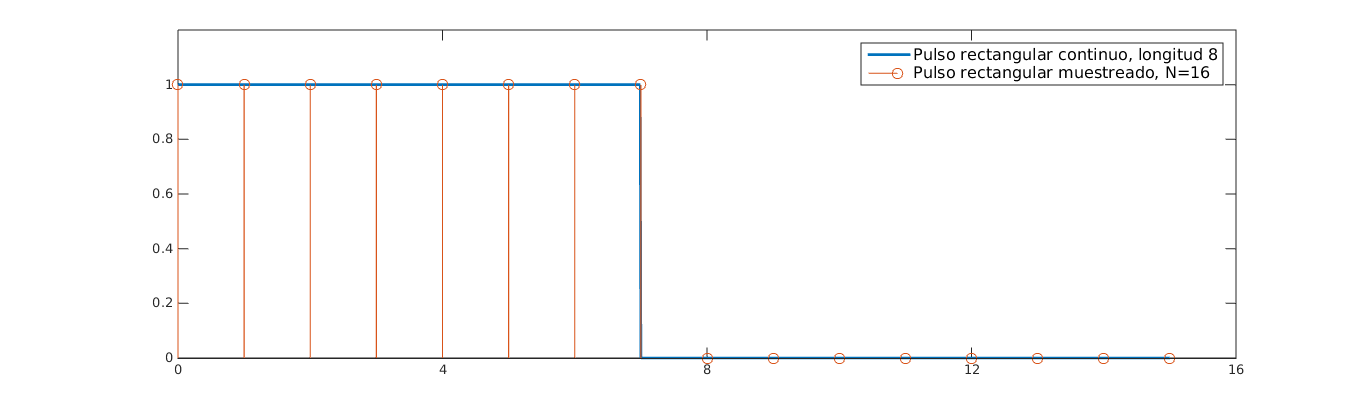
\includegraphics[width=12cm]{./figures/pulso_rect.png}
        \caption{Pulso rectangular de longitud 8, continuo y muestreado con N=16}
        \label{fig:escalon_16}
\end{figure}

\begin{figure}[htb!]
        \centering
        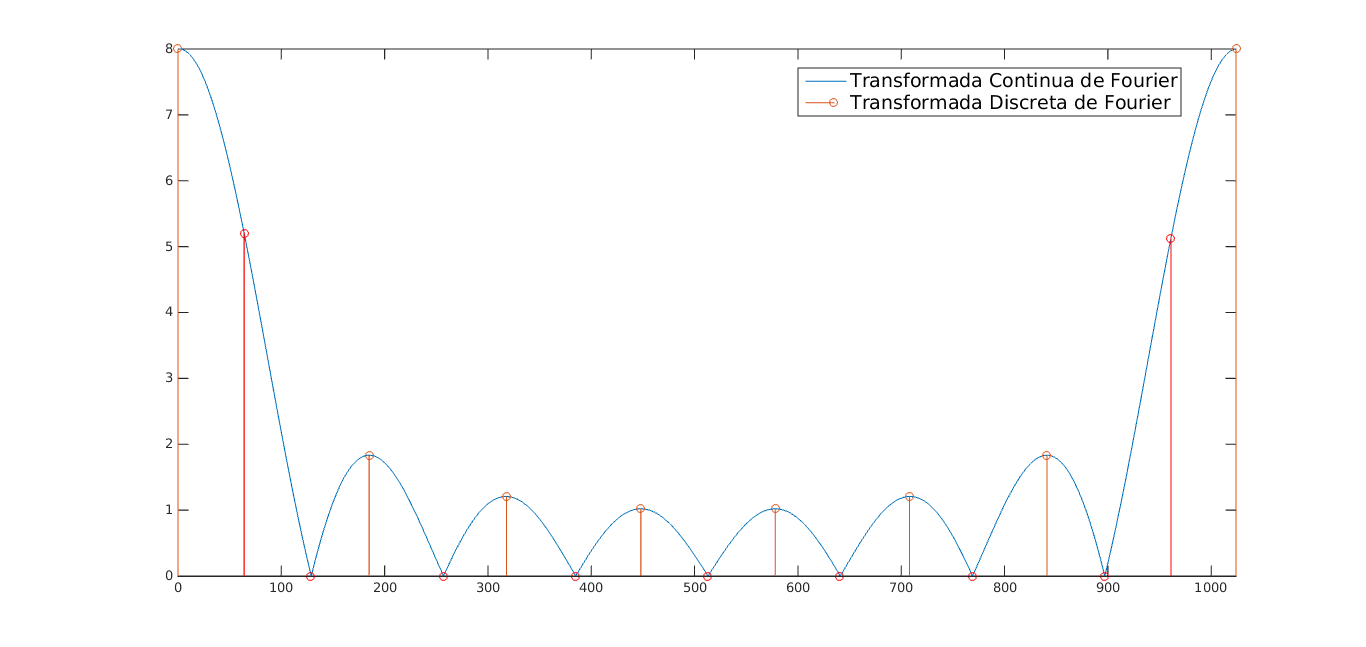
\includegraphics[width=12cm]{./figures/FT_DFT.png}
        \caption{Transformada de Fourier de un pulso rectangular}
        \label{fig:fourier_escalon}
\end{figure}

Se debe recordar los efectos del muestreo en tiempo y en frecuencia:
\begin{itemize}
  \item Al muestrear en tiempo se obtiene un espectro periódico con frecuencia
  de muestreo $f_s$. La aproximación de la transformada de Fourier a través
  de la DFT es razonable si las componentes en frecuencia de $x(t)$ están
  concentradas en un rango menor a la frecuencia de Nyquist $f_s/2$ de acuerdo con el
  teorema de muestreo de Shannon \cite{Shannon}.
  \item Al muestrear en frecuencia la función temporal se vuelve periódica, esto
  es, la DFT asume a la función $x(t)$ como periódica. Por este motivo se debe
  utilizar una frecuencia de muestreo y una ventana de análisis de forma que
  cubran un número entero de períodos de $x(t)$ (o períodos teóricos en caso
  que $x(t)$ no sea periódica) en N muestras para evitar anomalías en la
  transformada, tales como leakage, ripple, etc.
\end{itemize}

\section{La Transformada Rápida de Fourier} \label{sec:fft}

La implementación directa de la DFT según (\ref{eq:DTF}) implica que
para cada una de las N salidas del cálculo se requieren N operaciones
aritméticas, N sumas, lo que equivale a una complejidad del orden de
$\Theta(N^2)$, lo cual es inaceptables en sistemas escalables. Por esto históricamente se buscaron
formas más eficientes de realizar el cálculo de la DFT. Estos algoritmos se conocen globalmente como Tranformada Rápida de
Fourier (FFT, Fast Fourier Transform), que permiten reducir la
complejidad al orden de $\Theta(N*\log(N))$ \cite{Schaffer2_2}\cite{Schaffer2_1}.

Los algoritmos de FFT utilizan la estrategia \emph{divide y vencerás} a través de
una transformación de una DFT de longitud N (\ref{eq:DTF}) en una
representación multidimensional $N=\Pi_lN_l$. Esto permite dividir el cálculo de
una DFT de $N$ puntos en múltiples DFT de $N_l$ reduciendo de esta manera la
complejidad computacional total.

Como ejemplo se analizará brevemente la descompocisión en dos dimensiones.
Se transforma el índice temporal $n$ según

 \begin{equation}
n = An_1 + Bn_2 \ mod\ N \qquad 
	\begin{cases}
	0\leq n_1 \leq N_1 -1 \\
	0\leq n_2 \leq N_2 -1
	\end{cases}
\label{eq:timeInedx}
\end{equation}

Donde $N=N_1*N_2$ y $A,B \in Z$ son constantes a definir. Usando esta
transformación se construye un mapeo bidimensional del tipo $f:C^N\rightarrow
C^{N_1xN_2}$.

Aplicando una transformación similar al índice k en el dominio de la frecuencia:

\begin{equation}
k = Ck_1 + Dk_2 \ mod\ N \qquad 
	\begin{cases}
	0\leq k_1 \leq N_1 -1 \\
	0\leq k_2 \leq N_2 -1
	\end{cases}
\label{eq:freqInedx}
\end{equation}

Donde $C,D \in Z$ son constantes a definir. Como la DFT es biyectiva se debe
tener precaución en la elección de los coeficientes A, B, C y D para que la
nueva representación de la transformada siga teniendo esta característica.

Esta representación implica la separación de la DFT de $N$ puntos en dos DFT de
$N_1$ y $N_2$ puntos aplicadas una a continuación de la otra. Esta
representación se puede realizar de forma recursiva y subdividir a su vez $N_1$
como $N_1 = N_{11}N_{12}$ y así sucesivamente.

Los algoritmos de FFT permiten un cálculo eficiente de la DFT no solo en tiempo
de cálculo sino también en complejidad de código en caso de software y en
complejidad, tamaño y consumo en caso de hardware haciendo posible su implementación
en circuitos integrados.

Los diferentes algoritmos de FFT se diferencian entre sí por los valores
que asignan a los coeficientes $A,\ B,\ C\ y\ D$. Existen algoritmos que
permiten aprovechar esta optimización del cálculo dependiendo de la naturaleza
de la señal y el objetivo del cálculo para cualquier longitud de la DFT.

\section{Uso de la DFT en las comunicaciones digitales}
\subsection{Multiplexación por división ortogonal de frecuencia (OFDM)}

La creciente demanda de servicios de comunicación inalámbrica lleva a la
necesidad de aumentar el flujo de datos transmitidos a través de
radiofrecuencias. Tratar de llevar la velocidad de transmisión de símbolos para
alcanzar tasas de bits del orden del Mbit o mayores requiere la utilización de
ecualización adaptativa lo que eleva la complejidad y el costo de los equipos
utilizados \cite{Prasad2_1}.
Una forma de encarar el problema es la multiplexación en frecuencia, donde los
símbolos en los que se modula la información se multiplexan en múltiples
portadoras y se transmiten en forma simultánea aumentando de esta forma la tasa de transferencia de
bits sin necesidad de aumentar la frecuencia o la complejidad de los símbolos utilizados en la
modulación. Otra ventaja de la transmisión multiportadora es su robustez frente a interferencia selectiva en frecuencia ya
que solo se verían afectadas algunas de las portadoras y el error provocado se
puede corregir mediante un sistema de corrección de errores. 

En los sistemas tradicionales de transmisión multiportadora la banda de
frecuencia total se divide en $N$ canales sin superposición los cuales son
modulados por diferentes símbolos y multiplexados en frecuencia. La transmisión simultánea de
múltiples frecuencias presenta el riesgo de interferencia entre portadoras (ICI, Inter Charrier
Interference) por lo que los canales deben separarse de forma de reducir la interferencia entre
ellos, lo que lleva a un aprovechamiento ineficiente del espectro disponible.
Para mejorar la eficiencia en el uso del ancho de banda a mediados de la
década de 1960 se propuso la utilización de transmisión en paralelo, al igual
que en el sistema tradicional, y la multiplexación en frecuencia sobre canales
superpuestos, que llevando una velocidad de símbolo $b$ son espaciados entre si una
distancia $b$ en frecuencia para disminuir el ruido impulsivo y distorsión por
caminos múltiples además de aprovechar mejor el ancho de banda \cite{Prasad2_1}.                  
En la figura \ref{fig:portadoras} se ve la diferencia en el aprovechamiento 
del ancho de banda al transmitir $8$ subportadoras separadas y las mismas $8$ 
subportadoras superpuestas.

\begin{figure}[htb!]
        \centering
        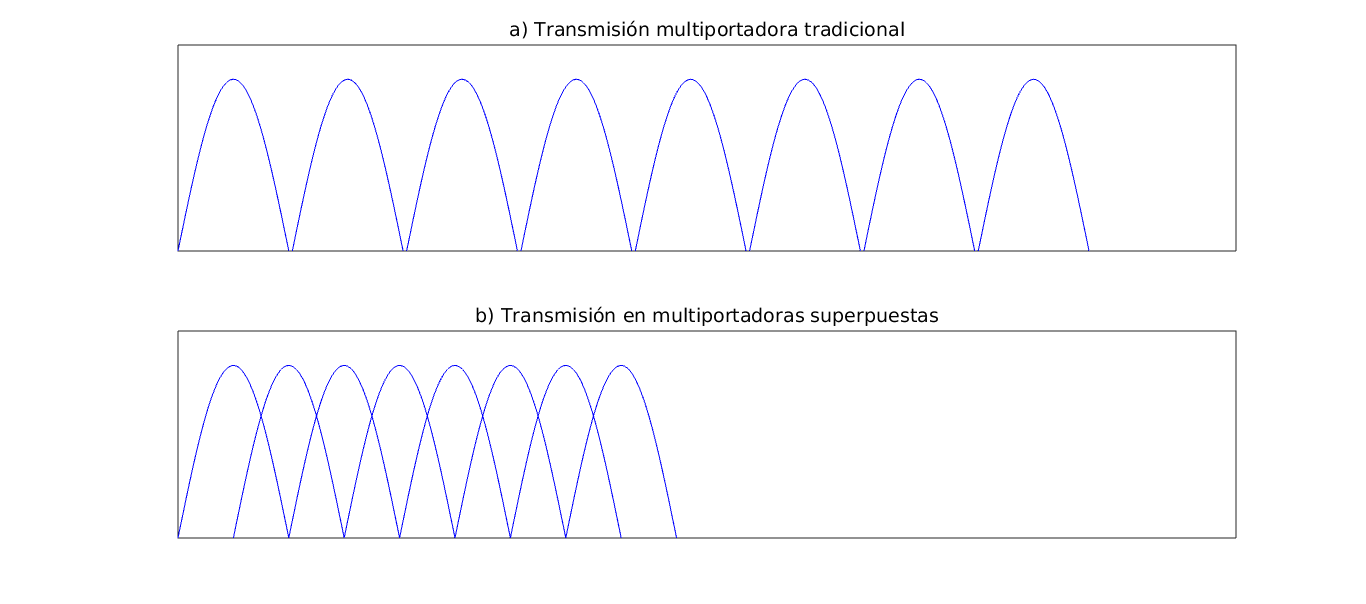
\includegraphics[width=17cm]{./figures/trad_mult.png}
        \caption{Dos formas de transmisión multiportadora}
        \label{fig:portadoras}
\end{figure}

El sistema de multiplexado en división de frecuencias ortogonales (OFDM, 
Orthogonal Frecuency-Division Multiplexing) propone la utilización de
frecuencias  matemáticamente ortogonales para reducir la interferencia entre las
portadoras. Con el receptor actuando como un banco de demoduladores
que traslada cada subportadora a banda base, se realiza una integración sobre un
período de la señal de esa subportadora para recuperar la información. Si las demás
portadoras tienen un número entero de ciclos durante ese período ($T$), luego de la
integración la contribución de estas a la subportadora que se está procesando es nula. Entonces las
portadoras serán ortogonales si están separadas un múltiplo de $1/T$. La figura \ref{fig:OFDM_ports} 
muestra un conjunto de subportadoras conformando una señal OFDM.

\begin{figure}[htb!]
        \centering
        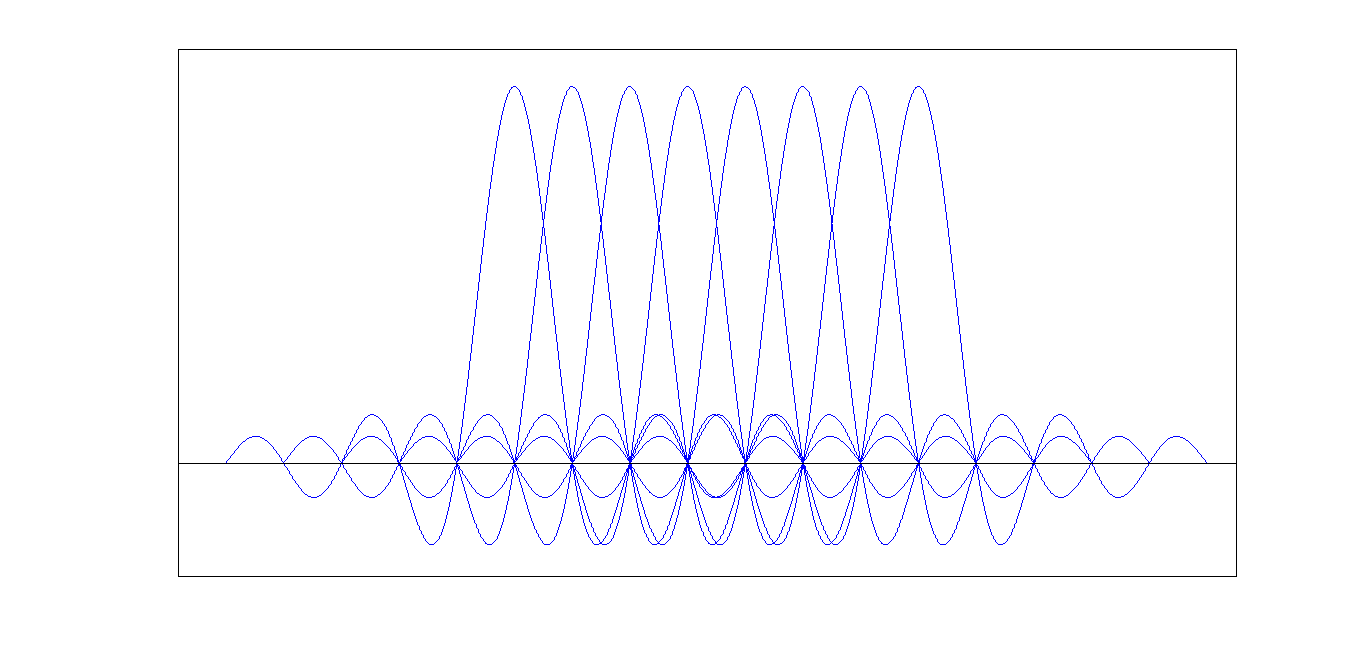
\includegraphics[width=17cm]{./figures/ofdm_subcarriers.png}
        \caption{Idea conceptual de una señal OFDM}
        \label{fig:OFDM_ports}
\end{figure}

El sistema de transmisión por OFDM se utiliza en muchos tipos de
comunicación actuales siendo uno de los sistemas más extendidos \cite{Prasad2_1}. Este sistema
está presente en las conexiones de datos tipo DSL, en las redes inalámbricas
(WLAN, WPAN) de tipo Wi-Fi, WiMax, etc, en las transmisiones de video y audio
digital (DAB/DVB) entre otros muchos medios de transmisión de información.

Si bien por si sola la modulación OFDM presenta varias ventajas en la
transmisión de datos esto no alcanza para una implementación práctica ya que
deben tenerse en cuenta las características distorisivas del canal.

Una de las modificaciones principales sobre el sistema teórico es el agregado de
un intervalo de guarda (GI sus siglas en inglés) utilizado para reducir el
efecto del delay producido por la característica multi-camino del canal. Este
GI está compuesto por la repetición de la porción final del símbolo transmitido
al principio del mismo, convirtiendo el símbolo en periódico. Esta porción
agregada se conoce como prefijo cíclico. Gracias al prefijo cíclico el efecto
dispersivo en tiempo del canal se reduce a una convolución cíclica por lo que
con solo descartar el GI en el receptor se obtiene el símbolo completo.
Además, gracias a las características de la convolución cíclica o circular, se
preserva la ortogonalidad de las subportadoras. La desventaja de aplicar el
prefijo cíclico es la disminución en la eficiencia del uso del ancho de banda
al agregar información no útil a la transmisión. La duración del GI
($T_{guard}$) es seleccionada para que sea mayor al máximo delay del canal. Por
lo tanto la parte efectiva de la señal recibida puede ser vista como la
convolución cíclica del símbolo transmitido por la respuesta impulsiva del
canal.

Por otro lado un pulso rectangular tiene un gran ancho de banda debido a los
lóbulos laterales de la sinc que compone su espectro. Para reducir la potencia
transmitida fuera del ancho de banda del símbolo se agrega un tiempo de ventana
a la transmisión con una forma de onda que cae progresivamente, a diferencia del
pulso rectangular, lo que reduce los lóbulos lateralesde la sinc reduciendo a su
vez el ancho de banda total del símbolo. Esta ventana se agrega al inervalo de
guarda descipto anteriormente aumentando la robustez respecto de la
dispersividad del canal pero reduciendo aún más la eficiencia ya que esta
ventana también es descartada por el receptor.

\begin{figure}[htb!]
        \centering
        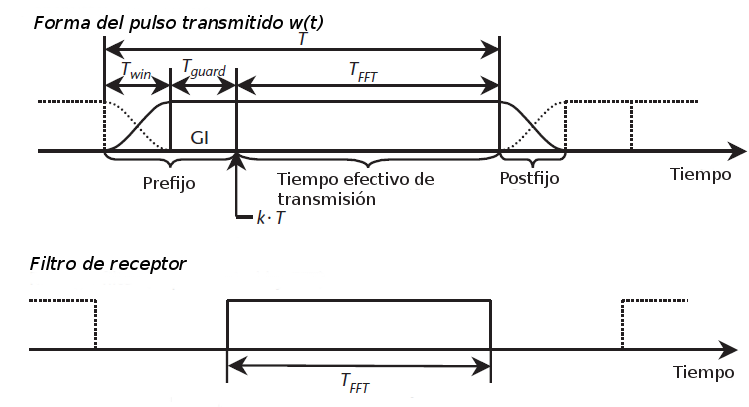
\includegraphics[width=12cm]{./figures/symbol_T.png}
        \caption{Diagrama de tiempos de un símbolo OFDM}
        \label{fig:symbol_T}
\end{figure}

Esto queda ejemplificado en la figura \ref{fig:symbol_T} donde se ve el esquema
de tiempos de un símbolo OFDM. Como este procesamiento se realiza habitualmente en
hardware digital estos tiempos suelen expresarse en muestras. $T$ ($N$),
$T_{FFT}$ ($N_{FFT}$), $T_{guard}$ ($N_{guard}$) y $T_{win}$ ($N_{win}$)
representan los tiempos (número de muestras) del símbolo transmitido, su parte
efectiva, el GI y el tiempo de ventana respectivamente.

En la figura \ref{fig:OFDM_blocks} se
observa un diagrama en bloques de un transmisor OFDM. La data de origen es dividida en paquetes/canales y mapeada a lo símbolos
respectivos de la constelación correspondiente a la modulación seleccionada para la transmisión.
Esos símbolos, que componen una constelación de símbolos complejos, es modulada en las
multiportadoras ortogonales para su transmisión y se le agrega el intervalo de guarda para luego
convertir la señal resultante digital en una señal analógica para ser transmitida. Una vez recibida
esta señal en el receptor, es digitalizada para su procesamiento y se remueve el intervalo de
guarda. La porción de información efectiva de la señal es enviada al demodulador OFDM que extrae la
constelación de puntos complejos que es demapeada en la información original.
El presente trabajo se enfoca en desarrollar los bloques de modulación y demodulación OFDM del
diagrama de bloques expuesto.


\begin{figure}[htb!]
        \centering
        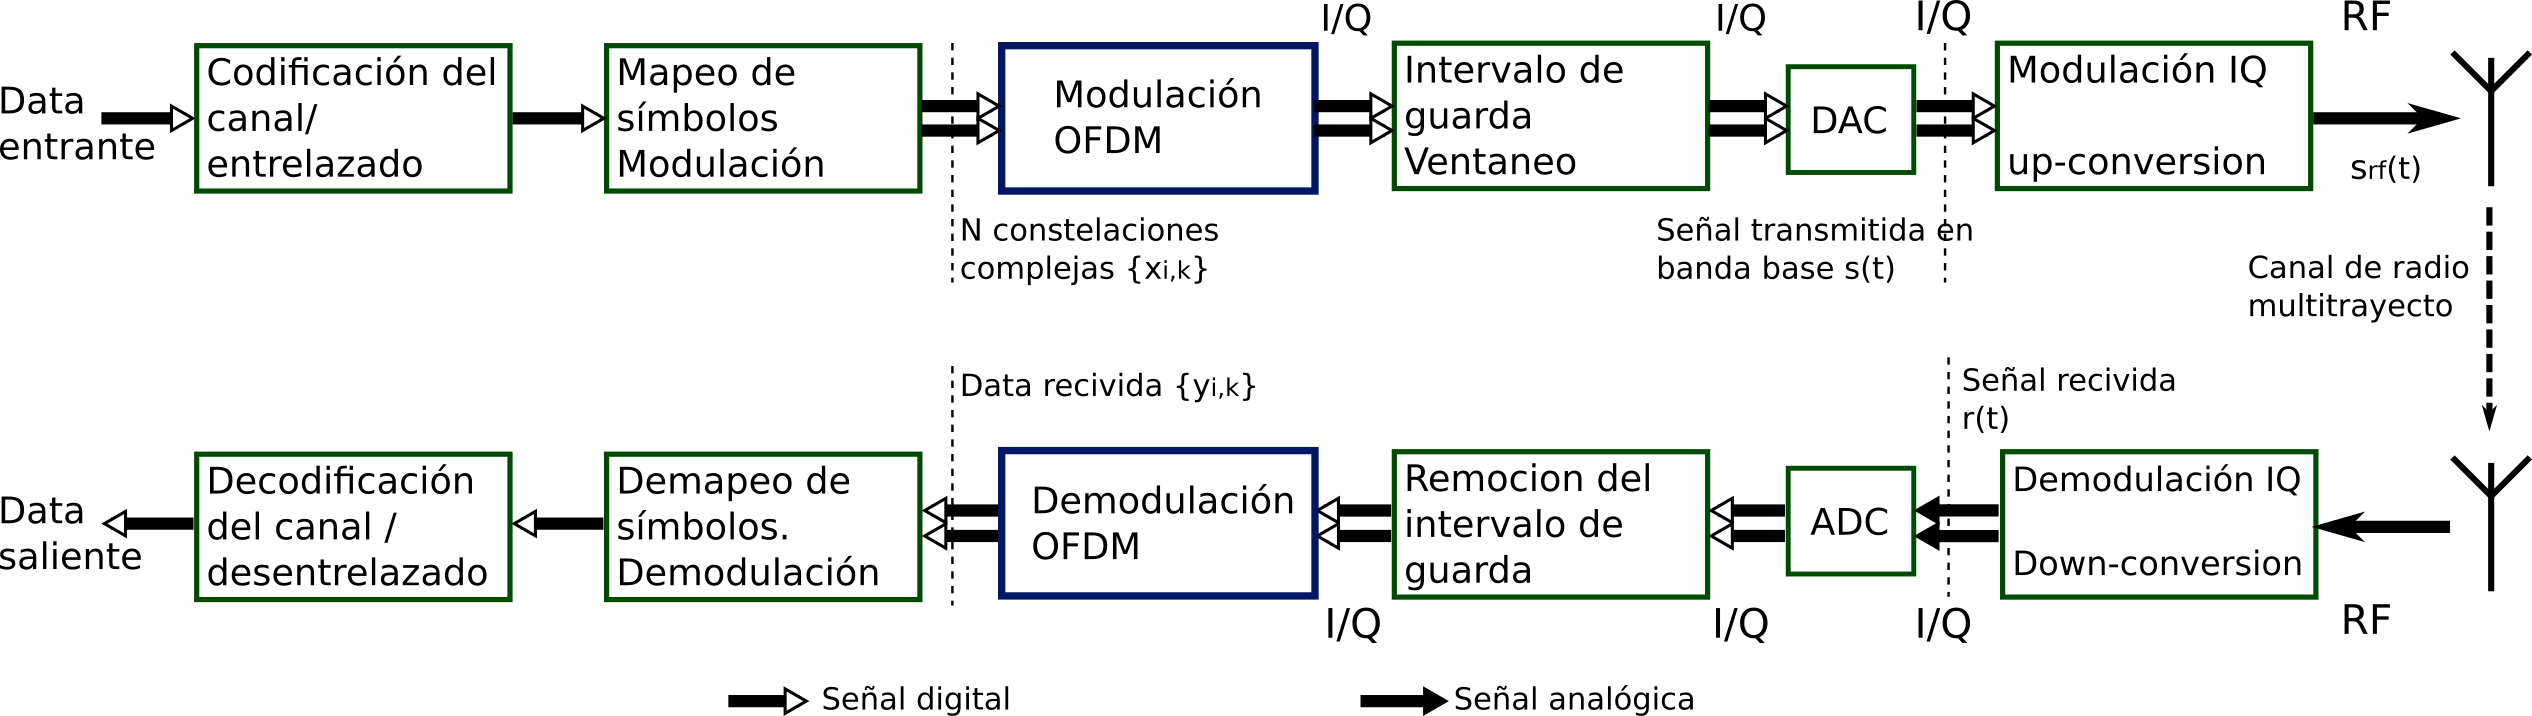
\includegraphics[width=15cm]{./figures/ofdm_blocks.png}	%OFDM_block_1
        \caption{Diagrama en bloques de una transmisión punto a punto OFDM}
        \label{fig:OFDM_blocks}
\end{figure}

\subsection{Implementación de la modulación OFDM mediante DFT}

Matemáticamente la OFDM se expresa como la suma de los pulsos base desplazados
en tiempo y frecuencia y multiplicados por los símbolos de datos.
En notación temporal, el k-ésimo símbolo de una señal OFDM se escribe como:

\begin{equation}
s_{RF,k}(t-kT) = 
%	\begin{cases}
	Re\left\{ w(t-kT) \sum\limits_{i=-N/2}^{N/2-1} x_{i,k} e^{j2\pi
	\left(f_c+\frac{i}{T_{FFT}}\right)(t-kT)}\right\}\\
%	\end{cases}
\label{eq:OFDM_symbol}
\end{equation}

para $kT-T\text{win}-T\text{guard}\leq t \leq kT+T_{FFT}+T\text{win}$ y $0$ para todo otro caso.

Donde:

\begin{itemize}
\item $T$: Duración de símbolo, tiempo entre dos símbolos consecutivos
\item $T_{FFT}$: Parte efectiva de un símbolo
\item $Tguard$: GI, duración del prefijo cíclico
\item $Twin$: intervalo de ventana
\item $k$: Índice del símbolo transmitido
\item $i$: Índice de subportadora, $i \in \{$$–N/2,\; –N/2+1,\; … –1,\; 0,\; 1,\; …
N/2–1$$\}$;
\item $x_{i,k}$: Punto de la constelación de la señal. Símbolo complejo
modulado en la i-ésima portadora del k-ésimo símbolo OFDM
\item $w(t)$: El pulso formador
\end{itemize}

Finalmente una secuencia continua de símbolos OFDM se expresa como:

\begin{equation}
s_{RF}(t) = \sum_{k=-\infty}^{\infty}s_{RF,k}(t-kT)
\label{eq:OFDM_seq}
\end{equation}

De estas ecuaciones se deduce la señal compleja equivalente en banda base:

\begin{equation}
s(t) = \sum_{k=-\infty}^{\infty}s_{k}(t-kT)
\label{eq:OFDM_low}
\end{equation}

donde

\begin{equation}
s_{k}(t-kT) =
%	\begin{cases}
	w(t-kT) \sum\limits_{i=-N/2}^{N/2-1} x_{i,k} e^{j2\pi
	\left(\frac{i}{T_{FFT}}\right)(t-kT)}
%	\end{cases}
\label{eq:OFDM_symbol_low}
\end{equation}

para $kT-T\text{win}-T\text{guard}\leq t \leq kT+T_{FFT}+T\text{win}$ y $0$ para todo otro caso. 

Se puede notar la similitud entre (\ref{eq:OFDM_symbol_low}) y 
(\ref{eq:iDTF}) de la IDFT donde $k$ representa la subportadora. Esta
similitud es sumamente importante ya que permite reemplazar los moduladores del
transmisor por el cálculo de una IDFT, o su versión de mayor eficiencia IFFT, y
el banco de filtros para demodular en el receptor por el cálculo de una DFT al realizar
procesamiento digital.
Esto representa una simplificación considerable en el diseño de sistemas OFDM y
su procesamiento mediante hardware digital o incluso por software  y ha motivado
el creciente estudio sobre la transformada discreta de Fourier y los algoritmos
de cálculo eficiente de la misma, buscando arquitecturas de procesamientos más eficiente, más
pequeñas, con menor consumo de energía/recursos, etc.


\chapter{Arquitecturas para el cómputo de la Transformada Rápida de Fourier} \label{sec:cap_arqs}

En el capítulo anterior fue expuesta la utilidad de la iDFT y la DFT para la mdulación y
demodulación de señales en un sistema OFDM y las ventajas de los algoritmos FFT para el cálculo de
la transformada discreta de Fourier.

Siguiendo la terminología introducida por Burrus \cite{Burrus} \cite{Meyer3_1} se define como
\textit{algoritmos FFT} a aquellos donde se realiza un mapeo multidimensional de los índices en sus
entradas y salidas, como se explicó en la sección \ref{sec:fft}, dejando el término \textit{algoritmo DFT}
a aquellos algoritmos donde no se utiliza un mapeo multidimensional de los índices.

\section{Algoritmos DFT}

Los algoritmos DFT implementan el cálculo de la DFT aplicando optimizaciones sobre la
ecuación de síntesis.

\subsection{Algoritmo de Goertzel}

Cada componente del espectro de una señal $x_{[n]}$ en un cómputo de DFT puede escribirse como

\begin{equation}
	X[k] = x[0] + x[1]W_{N}^{k} + x[2]W_{N}^{2k} + \ldots + x[N-1]W_{N}^{(N-1)k}  
\label{eq:goertz1}
\end{equation}

Se pueden combinar todos los $x[n]$ con el mismo factor común $W_N^k$ obteniendo

\begin{equation}
	X[k] = x[0] + W_{N}^{k}(x[1] + W_{N}^{k}(x[2] + \ldots + x[N-1]W_{N}^{k} \ldots ))  
\label{eq:goertz2}
\end{equation}

Esta ecuación resulta en una posible implementación recursiva para el cálculo de $X[k]$. Este
cómputo es conocido como el algoritmo de Goertzel. Su mayor utilidad se encuentra para calcular un
número reducido de componentes espectrales ya que para el cálculo de una DFT completa la complejidad
llega a $\Theta(N^2)$, donde no representa ninguna mejora respecto al cálculo directo de la DFT
\cite{meyer_Goerts}.

\subsection{Transformación Bluestein Chirp-z}

En la transformación Bluestein Chirp-z el exponente \textit{kn} en \ref{eq:DTF} es expandido
cuadráticamente a 

\begin{equation}
	kn = -(k-n)^2/2 + n^2/2 + k^2/2  
\label{eq:chirp1}
\end{equation}

El cómputo de la DFT se reduce entonces a

\begin{equation}
	X[k] = W_{N}^{k^2/2}\sum_{n=0}^{N-1}(x[n]W_{N}^{n^2/2})W_{N}^{-(k-n)^2/2}  
\label{eq:goertz2}
\end{equation}

Entonces el cálculo de la DFT mediante este algoritmo se reduce a tres pasos:

\newcommand{\Conv}{\mathop{\scalebox{1.5}{\raisebox{-0.2ex}{$\ast$}}}}

\begin{itemize}
  \item N multiplicaciones de $x[n]$ por $W_{N}^{n^2/2}$
  \item Convolución lineal de $x[n]W_{N}^{n^2/2} \Conv W_{N}^{n^2/2}$
  \item N multiplicaciones por $W_{N}^{k^2/2}$
\end{itemize}

Para una transformación completa se necesita una convolución de longitud N y 2N multiplicaciones
complejas. Una ventaja de este algoritmo es que puede utilizarse para cualquier valor de N, sin la
limitación de que N sea par o potencia de 2 o 4 \cite{meyer_CZT}.

\subsection{Algoritmo DFT de Winograd}

El algoritmo de Winograd transforma el cómputo de la DFT en una convolución cíclica y aplica el
algoritmo de convolución de Winograd \cite{WinoConv}. La longitud de la DFT queda
restringida a números primos o potencias de números primos.
La transformación de la DFT en una convolución se realiza mediante el método Rader \cite{Rader}, en
el que partiendo de la premisa que N es un número primo se puede hallar un elemento generador
$g$ que genere todos los elementos $n$ y $k$ \cite{gener}, a excepción del $0$,  de forma que

 \begin{equation}
	X[k] = \sum_{n=0}^{N-1}x[n]W_{N}^{nk} \qquad k,n \; \displaystyle\epsilon \;
	\mathbb{Z_N}
\label{eq:rader1}
\end{equation}

Reemplazando $n$ por $g^n \thinspace mod \thinspace N$ y $k$ por $g^k \thinspace mod \thinspace N$
se obtiene el siguiente mapeo de índices:

\begin{equation}
	X[g^k \thinspace mod \thinspace N] - x[0] = \sum_{n=0}^{N-2}x[g^n \thinspace mod \thinspace N]
	W_{N}^{g^{n+k} \thinspace mod \thinspace N}
\label{eq:rader2}
\end{equation}

para $k \epsilon \{1,2,3 \ldots N-1\}$. Se puede notar que el lado derecho de \ref{eq:rader2} es una
convolución cíclica, i.e.,

\begin{equation}
	[x[g^0 \thinspace mod \thinspace N], x[g^1 \thinspace mod \thinspace N], \ldots, x[g^{N-2}
	\thinspace mod \thinspace N] \Conv [W_N, W_N^g, \ldots, W_N^{g^{N-2}
	\thinspace mod \thinspace N}]
\label{eq:rader2}
\end{equation}

Implementando la convolución con el algoritmo de Winograd se reduce la cantidad de multiplicaciones
no triviales aumentando así la eficiencia del cómputo de DFT \cite{WinoConv}.

\section{Álgoritmos FFT}

Los algoritmos FFT logran la eficiencia en el cómputo de la DFT a través de un mapeo
multidimencional de los coeficientes.

\subsection{Algoritmo de Cooley-Tuckey para el cálculo de FFT}

El algoritmo de Cooley-Tukey es el más universal de los algoritmos para cálculo
de FFT porque permite utilizar cualquier factorización de N \cite{Meyer2_2}. En particular
los algoritmos de Cooley-Tukey que transforman N en una potencia de base $r$,
$N=r^\nu$, son llamados \emph{Radix-r} y son los más populares \cite{Meyer2_2}.

La transformación de índices propuesta por Cooley y Tukey (y por Gauss
previamente) es también la más simple. Partiendo de
(\ref{eq:timeInedx}) y (\ref{eq:freqInedx}) se utilizan como coeficientes
$A=N_2$, $B=1$, $C=1$ y $D=N_1$ resultando en el mapeo:

\begin{equation}
n = N_2n_1 + n_2 \qquad 
	\begin{cases}
	0\leq n_1 \leq N_1 -1 \\
	0\leq n_2 \leq N_2 -1
	\end{cases}
\label{eq:CT_time_inedx}
\end{equation}

\begin{equation}
k = k_1 + N_1k_2 \qquad 
	\begin{cases}
	0\leq k_1 \leq N_1 -1 \\
	0\leq k_2 \leq N_2 -1
	\end{cases}
\label{eq:CT_freq_inedx}
\end{equation}

Dado el intervalo que pueden tomar $n_1$ y $n_2$ el cálculo del módulo no
necesita estar explícito.

Reemplazando $n$ y $k$ en $W_N^{nk}$ de acuerdo a (\ref{eq:CT_time_inedx}) y
(\ref{eq:CT_freq_inedx}):

\begin{equation}
W_N^{kn}=W_N^{N_2n_1k_1+N_1N_2n_1k_2+n_2k_1+N_1n_2k_2} 
\label{eq:Wkn}
\end{equation}

Como $W_N^{nk}$ es de orden $N=N_1N_2$ se llega a que $W_N^{N_1}=W_{N_2}$ y
$W_N^{N_2}=W_{N_1}$ que aplicado en \ref{eq:Wkn}:

\begin{equation}
W_N^{kn}=W_{N_1}^{n_1k_1}W_N^{n_2k_1}W_{N_2}^{n_2k_2} 
\label{eq:Wkn_red}
\end{equation}

Reemplazando (\ref{eq:Wkn_red}) en (\ref{eq:DTF}) se llega a:

\begin{equation}
X[k1,k2]=\sum_{n_2=0}^{N_2-1}
W_{N_2}^{n_2k_2}\left(W_{N}^{n_2k_1}\sum_{n_1=0}^{N_1-1}x[n_1,n_2]W_{N_1}^{n_1k_1}\right)
\label{eq:DFT_mod}
\end{equation}

La sumatoria interior en (\ref{eq:DFT_mod}) es una DFT de $N_1$ puntos que está
multiplicada por el factor $W_{N}^{n_2k_1}$. Definiendo
$\tilde{x}[n2,k1]=W_{N}^{n_2k_1}\sum_{n_1=0}^{N_1-1}x[n_1,n_2]W_{N_1}^{n_1k_1}$
y reemplazando en (\ref{eq:DFT_mod}) se llega a:

\begin{equation}
X[k1,k2]=\sum_{n_2=0}^{N_2-1}
W_{N_2}^{n_2k_2}\tilde{x}[n2,k1]
\label{eq:DFT_tilde}
\end{equation}

(\ref{eq:DFT_tilde}) muestra la DFT de $N_2$ puntos de $\tilde{x}$, lo que
representa la característica principal de este algoritmo, para cualquier valor de $N_1$ y $N_2$ tales que $N=N_1N_2$ la
DFT de longitud N de $x(n)$ se puede calcular siguiendo los siguientes pasos:

\begin{itemize}
  \item Transformar los índices de la secuencia de entrada según
  (\ref{eq:CT_time_inedx})
  \item Calcular la DFT de $N_1$ puntos de la secuencia $x(n)$.
  \item Multiplicar los puntos resultantes del paso anterior por el twiddle
  factor correspondiente.
  \item Calcular la DFT de longitud $N_2$ de la secuencia resultante del paso
  anterior.
  \item Transformar los índices de la secuencia de salida según
  (\ref{eq:CT_freq_inedx})
\end{itemize}

Nada impide aquí subdividir cualquiera de las DFT de la ecuación
(\ref{eq:DFT_tilde}) en dos DFT de longitudes menores sucesivamente hasta
obtener DFT de longitudes convenientes para realizar los cálculos.

Una ventaja del algoritmo de Cooley-Tuckey es la posibilidad del alojamiento en memoria
\textit{in-place} en el cual los resultados del cálculo de una etapa se guarda en memoria en las
mismas pocisiones que los valores utilizados para el cálculo, utilizando en forma eficiente la
memoria ya que para el cálculo de una DFT de $N$ puntos solo se requiere una memoria de longitud
$N$.

\subsubsection{Algoritmos radix-r}

Aprovechando la posibilidad que brinda el algoritmo de Cooley-Tuckey de poder factorizar $N$
libremente se puede optar por una factorización del tipo $N=r^\nu$. A los algoritmos de
Cooley-Tuckey de este estilo se los conoce como algoritmos \textit{radix-r}.
De esta manera el cálculo de la DFT se descompone en $\nu$ DFTs consecutivas de $r$ puntos cada una.

Por ejemplo para $r=2$ y $\nu$ etapas, $N=2^\nu$, el mapeo de índices queda como

\begin{equation}
n = 2^{\nu-1}n_{1}+\ldots+2n_{\nu-1}+n_{\nu}
\label{eq:radix2_n}
\end{equation}

\begin{equation}
k = k_1 + 2k_2+\ldots+2^{\nu-1}k_{\nu}
\label{eq:radix2_k}
\end{equation}

El número total de twiddle factors para un algortimo radix-2 es:

\begin{equation}
log_2(N)N/2
\label{eq:twf_radix2}
\end{equation}

La ventaja de esto es poder reducir el cálculo de  una DFT a múltiples cálculos de DFTs de tamaño
más pequeño y de cálculo más simple. Teniendo en cuenta por ejemplo que en el cómputo de una DFT de
longitud $2$ o $4$ no es necesario realizar ninguna multiplicación no trivial a excepción del
producto por el twiddle factor, eligiendo $N$ como potencia de $2$ o $4$ se reduce la cantidad de
multiplicaciones a realizar aumentando así la eficiencia del algoritmo.
 
\subsection{Algoritmo de Good-Thomas}

La transformación de índices sugerida por Good y Thomas transforma una DFT de longitud $N=N_1*N_2$
en una DFT bidimencional sin \textit{twiddle factors}, como si hay en el algoritmo de Cooley-Tukey.
El costo de la ausencia de \textit{twiddle factors} es la necesidad de que los factores $N_1$ y
$N_2$ deben ser coprimos (i.e., $gcd(N_k,N_l) = 1$ para $k \neq l$) y el mapeo se torna más
complicado al tener que realizar el cálculo de los índices en el momento y no poder utilizar tablas
precalculadas para ello.
Si se intenta eliminar los \textit{twiddle factors} introducidos por el mapeo de índices, según
\ref{eq:timeInedx} y \ref{eq:freqInedx}, se obtiene:

\begin{equation}
%	\begin{tabular}{r@{=}l}
	W_N^{nk} = W_N^{(An_1+Bn_2)(Ck_1+Dk_2)} \\
	         = W_N^{ACn_1k_1+ADn_1k_2+BCn_2k_1+BDn_2k_2}
%	\end{tabular}
\label{eq:GT_FFT}
\end{equation}

de donde surgen las siguientes condiciones necesarias que deben ser satisfechas en forma simultánea:

\begin{equation}
\langle AD \rangle_N = \langle BC \rangle_N = 0 
\label{eq:GT_cond1}
\end{equation}

\begin{equation}
\langle AC \rangle_N = N_2 
\label{eq:GT_cond2}
\end{equation}

\begin{equation}
\langle BD \rangle_N = N_1 
\label{eq:GT_cond3}
\end{equation}

El mapeo sugerido por Good y Thomas cumple con estas condiciones y está dado como sigue:

\begin{equation}
A=N_2 \qquad B=N_1 \qquad C=N_2 \langle N_2^{-1} \rangle_{N_1} \qquad D=N_1 \langle N_1^{-1}
\rangle_{N_2}
\label{eq:GT_mapping}
\end{equation}

Entonces

\begin{equation}
n = N_2n_1 + N_1n_2 \thinspace mod \thinspace N \qquad 
	\begin{cases}
	0\leq n_1 \leq N_1 -1 \\
	0\leq n_2 \leq N_2 -1
	\end{cases}
\label{eq:GT_time_inedx}
\end{equation}

\begin{equation}
k = N_2 \langle N_2^{-1} \rangle_{N_1}k_1 + N_1 \langle N_1^{-1}
\rangle_{N_2}k_2 \thinspace mod \thinspace N \qquad 
	\begin{cases}
	0\leq k_1 \leq N_1 -1 \\
	0\leq k_2 \leq N_2 -1
	\end{cases}
\label{eq:GT_time_inedx}
\end{equation}

Sustituyendo el mapeo de índices de Good-Thomas en la ecuación de la DFT (\ref{eq:DTF}) se obtiene

\begin{equation}
X[k1,k2]=\sum_{n_2=0}^{N_2-1}
W_{N_2}^{n_2k_2}\left(\sum_{n_1=0}^{N_1-1}x[n_1,n_2]W_{N_1}^{n_1k_1}\right)
\label{eq:GT_FFT_mod}
\end{equation}

La sumatoria interior en (\ref{eq:GT_FFT_mod}) es una DFT de longitud $N_1$. Definiendo
$\tilde{x}[n2,k1]=\sum_{n_1=0}^{N_1-1}x[n_1,n_2]W_{N_1}^{n_1k_1}$
y reemplazando en (\ref{eq:GT_FFT_mod}) se llega a:

\begin{equation}
X[k1,k2]=\sum_{n_2=0}^{N_2-1}
W_{N_2}^{n_2k_2}\tilde{x}[n2,k1]
\label{eq:GT_DFT_tilde}
\end{equation}

En este caso el procedimiento para el cómputo de la DFT mediante este algoritmo es similar al
procedimiento del algoritmo de Cooley-Tuckey pero sin la multiplicación intermedia por el
\textit{twiddle-factor}.

Existe una versión de este agoritmo conocido como el Algoritmo FFT de Winograd donde se
utiliza el mismo mapeo de Good-Thomas pero la DFT bidimensional resultante se resuelve utilizando el producto
de \textit{Kronecker} \cite{Meyer_Kron}.

\section{Selección del algoritmo}

\subsection{Algoritmos DFT y FFT} \label{sec:dftOfft}

Una métrica habitual a la hora de comparar los algoritmos de cómputo de DFT suele ser la cantidad de
multiplicaciones que deben realizarse, parámetro en que el algoritmo FFT de Winograd tiene el mejor
desempeño \cite{Meyer_Kron}, pero, dado que el dispositivo donde se va a implementar el algoritmo
puede tener unidades de cálculo de productos o similares, no debe ser este el único aspecto a tener
en cuenta.
La primera desición que debe tomarse es que tipo de algoritmo se utilizará, DFT o FFT. Para este
trabajo de tesis se seleccionará un algoritmo FFT ya que el mapeo multidimencional de los índices
permite dividir el cómputo de la DFT en cómputos más pequeños reduciendo la complejidad de la
implementación y permitiendo el uso de \textit{pipelines}\footnote{\label{pipeline} El pipelining
consiste en la división de un módulo combinacional en submódulos combinacionales entre los cuales
se colocan registros de modo de dividir la ejecución de todo el bloque en varios ciclos de clock,
lo que permite aumentar su frecuencia de trabajo} entre cada etapa de cómputo aumentando la
velocidad de procesamiento.

En la Tabla \ref{table:fft_comp}  se muestra una comparativa entre los distintos algoritmos FFT que
será tomada en cuenta para seleccionar cual será el algoritmo a implementar.

\begin{table}[h]
\begin{tabular}{l c c c}
\textbf{Propiedad} & \textbf{Cooley-Tuckey} & \textbf{Good-Thomas} & \textbf{Winograd} \\ \hline
Restricción sobre N & No & \multicolumn{2}{c}{Si. $gcd(N_k,N_l)=1$}\\ \hline
Máximo orden de $W$ & N & \multicolumn{2}{c}{$max(N_k)$} \\ \hline
Necesidad de \textit{Twiddle Factors} & Si & No & No \\ \hline
\# Multiplicaciones & bueno & bueno & mejor \\
\# Sumas & bueno & bueno & bueno \\
\# Esfuerzo de cómputo de índices & mejor & bueno & malo \\
\textit{Data in-place} & Si & Si & No \\ \hline
\end{tabular}
\caption{Comparativa entre algoritmos FFT}
\label{table:fft_comp}
\end{table}
 
Se puede apreciar en la tabla \ref{table:fft_comp} que el algoritmo de Cooley-Tuckey presenta las
mejores caraterísticas para uso general, siendo balanceada en cuanto a la cantidad de operaciones
aritméticas y la sobrecarga por el cómputo de los índices, pero ofreciendo la posibilidad de
utilizarla para cualquier valor de N.
Por este motivo se utilizará el algoritmo de Cooley-Tuckey para la implementación de este trabajo
de tesis, ya que la aplicación final de la arquitectura será como parte de un transmisor OFDM donde
no se puede limitar el número de puntos a las restricciones de los otros algoritmos mencionados. Además,
utilizando un algoritmo del tipo radix-r, se puede aprovechar la descompocisión en DFTs del mismo
tamaño reutilizando módulos tanto en la replicación de código como en un uso más eficiente de la
arquitectura una vez implementada.

\subsection{Arquitecturas radix-r}

Como se menciona en la sección \ref{sec:dftOfft} la arquitectura a implementar será de tipo radix-r.
En estos algoritmos se deben calcular $\nu$ DFTs de $r$ puntos cada una donde $N=r^\nu$. El valor
de $r$ toma importancia ya que la correcta elección del mismo puede conducir a implementaciones más
o menos eficientes. En la tabla \ref{table:fft_oper} se muestra la cantidad de operaciones
necesarias para bloques de DFT de distintos tamaños. Se considera como multiplicaciones triviales aquellas que son por $\pm 1$
y $\pm j$.

\begin{table}[h]
\begin{tabular}{c c c c}
\textbf{Long. del bloque} & \textbf{Multiplicaciones} & \textbf{Multiplicaciones no triviales} &
\textbf{sumas} \\ \hline 
$2$ & $2$ & $0$ & $2$ \\
$3$ & $3$ & $2$ & $6$ \\
$4$ & $4$ & $0$ & $8$ \\
$5$ & $6$ & $5$ & $17$ \\
$7$ & $9$ & $8$ & $36$ \\
$8$ & $8$ & $2$ & $26$ \\
$9$ & $11$ & $10$ & $44$ \\ \hline
\end{tabular}
\caption{Cantidad de operaciones complejas para distintas longitudes de DFT}
\label{table:fft_oper}
\end{table}

Se puede ver que para $r=2$ y $r=4$ no hay necesidad de realizar multiplicaciones no triviales
dentro de cada bloque DFT, quedando únicamente los productos por los twiddle factors. El siguiente
valor de $r$ en orden de eficiencia es $r=8$ que requiere dos multiplicaciones complejas por DFT.
Hay que tener en cuenta que si bien para un mismo valor de $N$ al aumentar el valor de $r$
disminuye la cantidad de etapas de DFT, también aumenta la complejidad de la implementación ya que
en cada bloque se deben procesar DFTs de $r$ puntos.
Teniendo en cuenta esto se decide implementar la arquitectura en dos versiones, utilizando $N=2$ y
$N=4$, ya que al ser valores pequeños permiten implementar la arquitectura para diversos valores de
$N$ manteniendo la complejidad de la implementación en niveles razonables, y se realizará un
análisis comparativo del rendimiento entre ellas.
Esto también implica que no es necesario agregar un multiplicador a los bloques DFT. Es por estos
motivos también que la mayoría de las implementaciones comerciales de bloques de cálculo de DFT se realizan con 
arquitecturas radix-2 y radix-4 \cite{radix_meyer}.

\subsubsection{Formas de implementar el algoritmo radix-r}\label{sec:radix}

En la figura \ref{fig:r2_8} se muestra un esquema simplificado de un algoritmo radix-2 de 8 puntos. 

\begin{figure}[htb!]
        \centering
        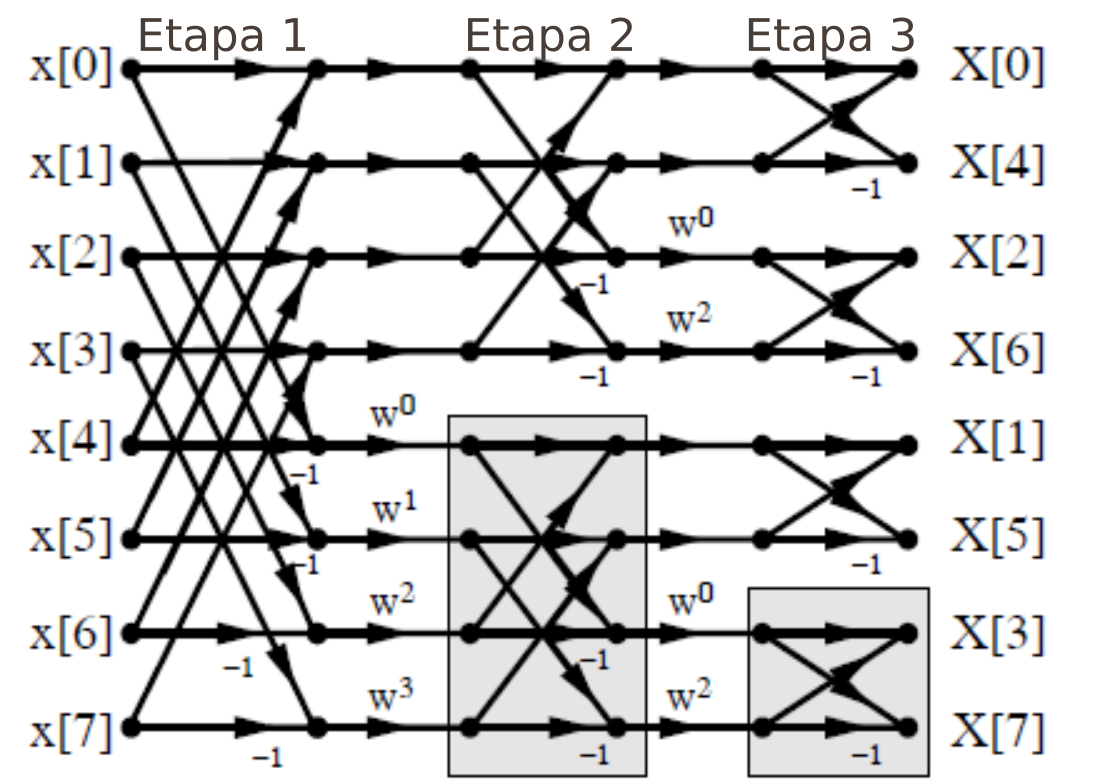
\includegraphics[width=10cm]{./figures/r2_8.png}
        \caption{FFT Radix-2 de 8 puntos}
        \label{fig:r2_8}
\end{figure}

En este esquema cada nodo donde llegan dos flechas representa una suma y cada flecha sobre una línea
representa un producto por el factor que la acompaña. Se aprecia claramente la división en etapas
en cada una de las cuales se realizan DFTs de $2$ puntos. Cada DFT de dos puntos es conocida como
\textit{butterfly} por la forma que toman las dos flechas cruzadas en el esquema de la figura
\ref{fig:r2_8}, en el caso de un algoritmo radix-4 el esquema es similar pero se realizan DFTs
tomando cuatro puntos. Se observa que para realizar una DFT de $8$ puntos se requieren $12$
\textit{butterflys}, generalizando $\frac{N}{2}*\log_2(N)$, y $8$ multiplicadores complejos,
generalizando $\frac{N}{2}*(\log_2(N)-1)$.
% Aquí se presentan variaciones en la forma en que se implementa el camino de
% los datos (\textit{datapath}) entre las distitintas etapas de cálculo de DFT. 
% La primer división surge en la cantidad de módulos DFT que se implementan. Las dos alternativas que
% surgen de esto son la implementación \textit{desenrollada} y la implementación \textit{iterativa}.
% 
% En la implementación desenrollada se utiliza un módulo de cómputo DFT (de $2$ o $4$ puntos según
% sea el caso) por etapa realizando de esta manera un cómputo DFT por etapa por ciclo de cálculo en
% paralelo, pasando los datos en serie de una etapa a la siguiente. La principal ventaja de esta
% implementación es que se tiene a la salida un punto por cada ciclo de cálculo. En la figura
% \ref{fig:r2sdf} se muestra un esquema de la arquitectura radix-2 SDF (Single-path Delay Feedback en
% inglés) \cite{torkelson} de 8 puntos donde se distinguen los bloques DFT de dos puntos y los
% multiplicadores para realizar el producto por el twiddle-factor. Se puede ver que la arquitectura
% consta de $log_2(8)=3$ etapas.
Existen diferentes variantes en la forma en que se implementa el camino de los datos
(\textit{datapath}), que implican diferencias en las cantidades de unidades de cómputo
\textit{butterfly} y de multiplicadores complejos. Las alternativas más comunes se listan a
continuación:

\begin{itemize}
  \item \textbf{Paralela} Se implementan todas las unidades \textit{butterfly} y multiplicadores
  complejos necesarios, dispuesto en una arquitectura similar al esquema de la figura
  \ref{fig:r2_8}. Se puede implementar en forma \textit{pipelined} colocando un banco de registros
  entre etapas concecutivas. La comunicación entre las etapas se realiza mediante un bus paralelo de
  tamaño $N$.
  \item \textbf{Desenrrollada} Arquitectura SDF (Single-path Delay Feedback en inglés)
  \cite{torkelson}. Se muestra un esquema de esta arquitectura para una FFT de $8$ puntos en la
  figura \ref{fig:r2sdf}. La comunicación se realiza mediante un bus serie, admitiendo un dato de
  entrada en cada ciclo de \textit{clock}. Se utiliza una unidad \textit{butterfly} por etapa,
  requiriendo en total $\log_\nu(N)$, y un multiplicador complejo por etapa excepto en la última
  dando un total de $ \log_\nu(N)-1$ multiplicadores. Se puede implementar en forma pipelined
  colocando un registro en medio de etapas concecutivas.
  \item \textbf{Iterativa} Se utiliza una única unidad \textit{butterfly} y un único multiplicador
  complejo para realizar secuencialmente las operaciones de todas las etapas. En la figura \ref{fig:r2sBf} se ve un esquema de la
  arquitectura radix-2 iterativa para $8$ puntos. 
\end{itemize}

\begin{figure}[htb!]
        \centering
        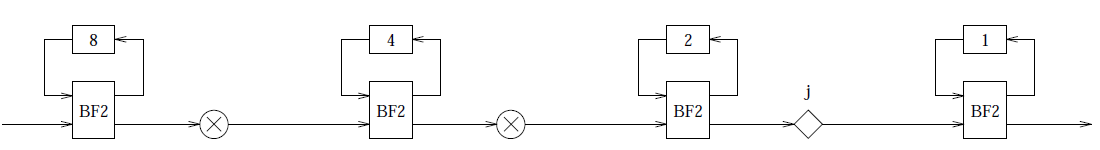
\includegraphics[width=13cm]{./figures/r2sdf.png}
        \caption{Arquitectura Radix-2 desenrollada SDF}
        \label{fig:r2sdf}
\end{figure}

% En la implementación iterativa se utiliza un único módulo de cómputo DFT con el que se calculan
% alternativamente cada una de las etapas, de a una por ciclo de cálculo. La principal ventaja de esta
% implementación es el menor tamaño respecto de la implementación desenrollada, lo que implica además
% menor consumo y una mayor eficiencia en la ocupación de los recursos. Por otro lado tiene como
% desventaja comparada con la versión desenrollada que ya no se tiene a la salida un punto nuevo por
% ciclo de cálculo sino que hay que esperar tantos ciclos de cálculo como etapas tenga la DFT a
% implementar, o sea, $\nu = log_r(N)$. En la figura \ref{fig:r2sBf} se ve un esquema de la
% arquitectura radix-2 iterativa para $8$ puntos. Aquí se realizan iterativamente todas las DFT de dos
% puntos con el mismo bloque ocupando un tercio del lugar que ocupa la arquitectura desentollada. En
% esta arquitectura se aprovecha el alojamiento en memoria in-place donde se reutiliza la pocisión de
% memoria ocupada por un punto luego de utilizarlo, para almacenar el valor resultante de ese cálculo.

\begin{figure}[htb!]
        \centering
        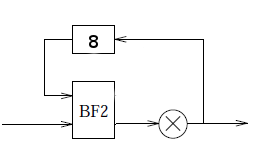
\includegraphics[width=6cm]{./figures/r2sBf.png}
        \caption{Arquitectura Radix-2 iterativa}
        \label{fig:r2sBf}
\end{figure}

En la tabla \ref{table:radixcomp} se realiza la comparativa entre las características distintivas de
cada implementación. El \textit{throughput} se toma como la cantidad y frecuencia con que se
obtienen puntos a la salida de la arquitectura. El campo \textit{pipelined} indica si la
implementación puede ser implementada de esa manera. En el caso del tamaño de memoria requerido no
se consideran implementaciones \textit{pipelined}, ya que en ese caso para la implementación
paralela hay que colocar N registros por cada etapa de \textit{ppipeline} que se coloca, mientras
que en la implementación desenrrollada se necesita un registro por etapa de \textit{pipeline}.

\begin{table}[htb!]
\centering
\begin{tabular}{l c c c}
\textbf{Característica} & \textbf{Radix paralela} & \textbf{Radix desenrrollada} &
\textbf{Radix iterativa}\\
\hline 
\# \textit{butterfly} & $\frac{N}{\nu}*\log_\nu(N)$ & $\log_\nu(N)$ & $1$ \\
\# multiplicadores & $\frac{N}{\nu}*(\log_\nu(N)-1)$ & $log_\nu(N)-1$ & $1$ \\
tamaño de memoria & $0$ & $N-1$ & $N$ \\
tipo de bus & Paralelo & Serie & Serie \\
\textit{throughput} & $N$ puntos por ciclo & $1$ punto por ciclo & $1$ punto cada $\log_\nu(N)$
ciclos\\
\textit{pipeline} & Si & Si & No\\
\hline
\end{tabular}
\caption{Comparativa entre las implementaciones paralela, desenrrolada e iterativa del algoritmo
radix-r}
\label{table:radixcomp}
\end{table}

Se puede observar que al aumentar el valor de $N$, la cantidad de puntos de la FFT a calcular,
aumenta la cantidad de unidades \textit{butterfly} y multiplciadores en las implementaciones
paralela, donde aumenta en forma proporcional, y en la desenrrollada, donde aumenta en forma
logarítmica, donde también aumenta el tamaño de la memoria. En la implementación iterativa un
aumento en la cantidad de puntos a procesar solo implica un aumento en memoria.

Teniendo en cuenta que el diseño de la arquitectura está orientado a su utilización en un sistema de
comunicación MIMO, no hay necesidad de un bus paralelo ya que los puntos de entrada llegan a la
arquitectura en serie, y son leídos de la misma manera, por el propio funcionamiento del sistema de
comunicación. En este sentido la implementación paralela queda prácticamente descartada. 
En cuanto al throughput, se puede operar la unidad de procesamiento FFT a una velocidad de
\textit{clock} mayor al resto del sistema para obtener el \textit{thoughput} necesario.

Se puede ver que la relación de tamaño entre la implementación desenrrollada y la iterativa
es del orden de $log_r(N):1$ para los módulos de cómputo aritmético. En base a la comparativa
realizada y al requerimiento de que la arquitectura sea económica en términos espaciales y de consumo se opta
por la implementación iterativa, ya que al aumentar $N$ solo se incrementa la cantidad de memoria
requerida manteniendo una arquitectura de tamaño reducido y bajo consumo. 

\subsection{Multiplicación por los twiddle factors} \label{sec:twiddlesec}

La implementación de multiplicadores en lógica digital es un tema delicado en cuanto al rendimiento
espacial y temporal. El cómputo de la DFT por el método de Cooley-Tuckey
requiere multiplicaciones complejas por los twiddle factors por lo que la forma de
implementar los multiplicadores no es un tema trivial. En una arquitectura desenrollada se necesitan
$log_r(N) - 1$ multiplicadores, dándole principal importancia al aspecto espacial de la
implementación, en tanto que en una arquitectura iterativa solo se necesita un único multiplicador
por lo que el aspecto principal a tener en cuenta es la velocidad de cómputo del multiplicador para
permitir una mayor frecuencia de cómputo.
Se analizan tres métodos para el cómputo del producto por los \textit{twiddle factors}.

\subsubsection{Algoritmo Cordic} \label{sec:cordicsec}

El producto por los twiddle factors, de la forma $W_N^{kn}=e^{\frac{-j2\pi kn}{N}}$, genera una
rotación en el plano complejo por lo que se puede reemplazar la multiplicación por una rotación.
En este sentido la primera opción que surge es la del algoritmo Cordic (Coordinate Rotation Digital
Computer sus siglas en inglés) que realiza rotaciones en dos dimenciones (además de otras
operaciones trigonométricas) en base únicamente a sumas/restas y desplazamientos.
Este algoritmo fue presentado en 1966 por Volder \cite{Volder} y es ampliamente utilizado para el
cálculo de funciones trigonométricas en sistemas digitales.

El principio de funcionamiento del algoritmo es realizar microrotaciones al vector inicial hasta
alcanzar una condición particular dependiente de una de las dos modalidades de funcionamiento: en
modo vectorial las coordenadas $(x_0,y_0)$ son rotadas hasta que $y_0$ converge a cero, en modo
rotacional el vector inicial $(x_0,y_0)$ es rotado un ángulo
$\theta_n$.
Esta rotación se lleva a cabo mediante microrotaciones por un ángulo $\theta_i$

\begin{equation}
x_{i+1} = x_i* \cos \theta_{i+1} - y_i* \sin \theta_{i+1}
\label{eq:micrototX}
\end{equation}

\begin{equation}
y_{i+1} = y_i* \cos \theta_{i+1} + x_i* \sin \theta_{i+1}
\label{eq:micrototY}
\end{equation}

Factorizando $\theta_{i+1}$ en (\ref{eq:micrototX}) y (\ref{eq:micrototY}) se obtiene:

\begin{equation}
x_{i+1} = \cos \theta_{i+1} (x_i - y_i* \tan \theta_{i+1})
\label{eq:micrototXfact}
\end{equation}

\begin{equation}
y_{i+1} = \cos \theta_{i+1} (y_i + x_i* \tan \theta_{i+1})
\label{eq:micrototYfact}
\end{equation}

Si se restringe $\tan \theta_{i+1}$ a $\pm 2^{-i}$ los productos del paréntesis pueden ser
reemplazados por desplazamientos aritméticos para cálculos en sistemas digitales de forma de
eliminar la necesidad de multiplicaciones en todas las iteraciones. El término $\cos \theta_{i+1}$
puede ser reemplazado por $\cos \theta_{i+1} = \cos (\arctan 2^{-i})$ definiendo las siguientes
variables:

\begin{equation}
K_i = \cos (\arctan 2^{-i}) = \frac{1}{\sqrt{1+2^{-2i}}}
\label{eq:micrototK}
\end{equation}

\begin{equation}
d_i = \pm 1
\label{eq:micrototd}
\end{equation}

Sabiendo que el coseno es una función impar, por lo que $\cos (\alpha) = \cos (-\alpha)$, y
reemplazando (\ref{eq:micrototK}) y /\ref{eq:micrototd}) en (\ref{eq:micrototXfact}) y
(\ref{eq:micrototYfact}) se obtienen las ecuaciones finales para el algoritmo Cordic:

\begin{equation}
x_{i+1} = K_i (x_i - y_i*d_i*2^{-i})
\label{eq:micrototXK}
\end{equation}

\begin{equation}
y_{i+1} = K_i (y_i + x_i*d_i*2^{-i})
\label{eq:micrototYK}
\end{equation}

La multiplicación por $K_i$ puede ser interpretada como una ganancia para todas las iteraciones por
lo que puede ser aplicada al final como una ganacia $K$ total del algoritmo igual a:

\begin{equation}
K = \prod K_i = \prod \frac{1}{\sqrt{1+2^{-2i}}}
\label{eq:Kprod}
\end{equation}

En cada iteración se debe decidir si $d_i = 1$ o $d_i = -1$, para lo cual se utiliza la diferencia
entre el ángulo deseado y el ángulo actual. Para ello se define una nueva variable como 

\begin{equation}
z_{i+1} = z_i - d_i \arctan 2^{-i}
\label{eq:zi}
\end{equation}

Y para decidir el valor de $d_i$ se utiliza

\begin{equation}
d_i =  
	\begin{cases}
	-1 \quad \sin z_i < 0 \\
	1 \quad \sin z_i \geq 0 
	\end{cases}
\label{eq:ni}
\end{equation}

$\arctan 2^{-i}$ puede ser calculado previamente y almacenado en tablas en memoria, al igual que el
valor de $K$, que al ser un valor definido para una cantidad determinada de iteraciones su
producto por el vector resultante puede ser calculado utilizando algoritmos eficientes para el
cómputo de productos.
En la figura \ref{fig:cordic} puede verse como se logra una rotación a través de microrotaciones a
lo largo de $4$ iteraciones.

\begin{figure}[htb!]
        \centering
        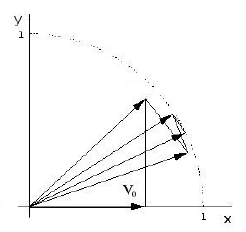
\includegraphics[width=6cm]{./figures/cordic.png}
        \caption{Ejemplo de rotación con algoritmo Cordic}
        \label{fig:cordic}
\end{figure}

Este algoritmo presenta como ventaja que solo utiliza sumas y desplazamientos para el cálculo de una
rotación vectorial, y la posibilidad de implementar las
etapas iterativas a través de un \textit{pipeline} para aumentar la frecuencia de trabajo. 

\subsubsection{Algoritmo BKM}

El algoritmo BKM busca, al igual que el algoritmo Cordic, resolver funciones elementales a través de
la utilización de sumas y desplazamiento de forma de poder implemetnarlas eficientemente en sistemas
digitales.
Este algoritmo se basa en las siguientes ecuaciones de recurrencia:

\begin{equation}
	\begin{cases}
	L_{n+1} = L_n(1+d_n*2^{-n}) \\
	E_{n+1} = E_n - \ln (1+d_n*2^{-n})
	\end{cases}
\label{eq:BKM}
\end{equation}

con $d_n \epsilon \{-1,0,1,-i,i,1-i,1+i,-1-i,-1+i\}$. 
Hay dos modos de operación del algoritmo. En el modo $L$ se itera hasta obtener $L_n=1$, entonces se
obtiene $E_n=E_1+\ln (L1)$. En el modo $E$ se itera hasta obtener $E_n=0$, entonces se obtiene
$L_n=L_1*\exp{E_1}$.
Es necesario precalcular y almacenar en memoria los valores de $\ln(1+d_n*2^{-n})$ para restárselo a
$E_1$ en cada iteración. La deducción y demostración del agoritmo es compleja y se puede ver en
\cite{BKM} así como ejemplos de aplicación para el cálculo de varias operaciones complejas y trigonométricas.
Para el cálculo del producto por los twiddle factors se utiliza la capacidad del algoritmo de
calcular la rotación de un vector $[a,b]$ por un ángulo $\theta$, utilizándo el modo $E$ con
$L1=a+ib$ y $E1=i\theta$.

Comparándolo con el algoritmo Cordic, ambos brindan la posibilidad de reducir el producto por los
twiddle factors a sumas y desplazamientos, con una complejidad espacial y computacional similar,
aunque el BKM requiere mayor almacenamiento en memoria que el Cordic. Los dos tienen la
característica de necesitar $p$ iteraciones para obtener $p$ bits de resolución. La principal
diferencia se da en la complejidad de implementación del algoritmo, donde el BKM es más complejo que
el Cordic, y en el hecho de que la principal ventaja del algoritmo BKM se da en implementaciones con
sistemas numéricos redundantes \cite{BKM}. Dado que la arquitectura a implementar en el presente
trabajo de tesis se hará utilizando el sistema numérico conocido como \textit{complemento a 2} (no
redundante) el algoritmo BKM no provee ninguna ventaja por sobre el algoritmo Cordic, siendo por el
contrario más complejo de implementar. Por este motivo de desestima su uso en este proyecto.

\subsubsection{Multiplicador complejo eficiente}

El uso extendido del algoritmo Cordic en arquitecturas de cómputo de FFT se justifica por el costo
espacial de implementar multiplicadores en sistemas digitales.
Pero dado que en este caso se necesita solo un multiplicador para toda la arquitectura, la
diferencia en el espacio requerido por el algoritmo Cordic y un multiplicador complejo no es
significativa (caso distinto para una implementación desenrollada donde se requieren $log_r(N)$
multiplicaciones).

En el caso del producto por los twiddle factors se requiere realizar una multiplicación compleja de
la forma:

\begin{equation}
R+jI = (A+jB)*(C+jD) = (A*C-B*D) + j(A*D+B*C)
\label{eq:prodcomp4}
\end{equation}

donde $(C+iD)$ es el twiddle factor. La implementación directa implica el uso de $4$
multiplicadores.
Se pueden precalcular y almacenar en una tabla determinados valores respecto a los twiddle factor
obteniendo una implementación más eficiente del producto complejo, como se explica a continuación.

Se precalculan y almacenan en memoria los valores $C$, $C+D$ y $(C-D)$. Con estos tres factores
precalculados se calcula:

\begin{equation}
\begin{split}
E &= A-B \\
Z &= C \times E = C \times (A-B)
\end{split}
\label{eq:prodcompZ}
\end{equation}

Y se computa el producto final como:

\begin{equation}
R = (C-D) \times B + Z
\label{eq:prodcompR}
\end{equation}

\begin{equation}
I = (C+D) \times A - Z
\label{eq:prodcompI}
\end{equation}

Como se indicó al principio de esta sección, al requerirse una única multiplicación compleja la
diferencia entre los costos espaciales de un multiplicador complejo y el algoritmo Cordic no es
significativa, por lo que se decide implementar el multiplicador complejo y evaluar su performance
respecto del algoritmo Cordic para decidir cual es mejor desde el punto de vista tanto de la
implementación como de la performance. Teniendo en cuenta que muchas FPGA cuentan con
unidades de procesamiento de señales, incluyendo multiplicadores, la implementación
de un multiplicador complejo tiene amplias ventajas sobre las demás opciones.

\subsection{Método de redondeo o truncamiento} \label{sec:redond}

El proceso de cómputo de la DFT mediante el método Radix requiere una serie
de sumas y restas, por lo que existe el riesgo de que se produzca desbordamiento (\textit{overflow}
en inglés) de la unidad aritmética. Para alamecenar el resultado de una suma entre dos operandos de $N$ bits
sin riesgo de desbordamiento se debe guardar el resultado en un número de $N+1$ bits. Esto
implicaría incrementar en $1$ el ancho de palabra de la aquitectura en cada etapa de cómputo.\\ 
Otra opción es la implmentación de un mecanismo de reducción del valor luego de una operación de suma y/o
resta dividiéndolo por $2$, ya que puede realizarse en forma trivial mediante un dezplazamiento
hacia la derecha. Debe tenerse en cuenta que este método introduce error en el resultado ya que la
dividir por $2$ se pierde información.\\
Se decide utilizar la segunda opción por su simplicidad de implementación y porque su tamaño no
depende de la cantidad de etapas a implementar. Para esto se evalua la implementación de un
mecanismo de redondeo y/o truncamiento para procesar el valor resultante de la división.

El redondeo y el truncamiento se utilizan para eliminar cifras no significativas en un número. En
este caso, su utilidad es la de eliminar el último bit del número que se divide por $2$ para
evitar el overflow.

El truncamiento consiste en eliminar las cifras no siginicativas descartándolas directamente.
El redondeo consiste en eliminar las cifras no significativas pero se suma $1$ al número resultante,
en caso que la última ciffra eliminada sea mayor o igual a la mitad de la base del sistema numérico, 
o no se suma nada en caso contrario.

En la Tabla \ref{table:redond} se muestran algunos ejemplos de la diferencia entre truncamiento y
redondeo al quitar el último digito decimal a cada número.

\begin{table}[htb!]
\centering
\begin{tabular}{c c c c}
\textbf{Número original} & \textbf{Truncamiento} & \textbf{Redondeo} \\ \hline 
$2.3641$ & $2.364$ & $2.364$ \\
$4.3156$ & $4.315$ & $4.316$ \\
$7.6355$ & $7.635$ & $7.636$ \\ \hline
\end{tabular}
\caption{Ejemplos de truncamiento y redondeo en sistema decimal}
\label{table:redond}
\end{table}

En el caso del redondeo en aritmética binaria, si el primer dígito eliminado es $1$ se le suma $1$
al número resultante y si es $0$ no se suma.

Se puede observar que el método de truncamiento introduce un error mayor al que introduce el método
de redondeo ya que el primero tiene una desviación máxima del valor real de una unidad mientras que
en el segundo la desviación máxima es de la mitad de una unidad.

Dado que la probabilidad de overflow depende de la magnitud de los puntos de entrada y que aplicar
cualquier de los dos métodos de aproximación introduce error se decide implementar un mecanismo de
división del resultado de la suma configurable en forma dinámica, en cuya configuración se puede
habilitar y deshabilitar la opción etapa por etapa y decidir si se aplica truncamiento o redondeo en
caso de habilitar la división.

\subsection{Arquitecturas a implementar}

De lo expuesto a lo largo del capítulo se decide implementar las siguientes arquitecturas:

\begin{itemize}
  \item Arquitectura radix-2 iterativa
  \item Arquitectura radix-4 iterativa
  \item Algoritmo cordic para el producto por los twiddle factor para las dos arquitecturas
  \item Multiplicador complejo para el producto por los twiddle factor para las dos arquitecturas
  como alternativa al algoritmo Cordic
  \item Mecanismo de división por dos a la salida del sumador/restador con posibilidad de
  seleccionar truncamiento o redondeo en forma dinámica.
\end{itemize}

La implementación de las arquitecturas se describe en el siguiente capítulo.

\chapter{Implementación a nivel de microarquitectura}

En el capítulo \ref{sec:cap_arqs} se analizaron diferentes tipos de arquitecturas existentes para el
cómputo de la DFT y se seleccionaron dos arquitecturas para ser implementadas. A su vez fueron analizadas
algunas alternativas para la implementación de diferentes aspectos del cómputo.

En este capítulo se describe la implementación a nivel de microarquitectura de los
módulos que componen las dos arquitecturas seleccionadas y la forma en que esos módulos se
interconectan. También se presentan las herramientas utilizadas para el diseño e implementación
de las arquitecturas.

El proceso de desarrollo se dividió en tres etapas. Primero, una vez seleccionadas las
arquitecturas, se conformó un diagrama en bloques identificando los módulos constitutivos, luego se implementó cada
uno de esos módulos realizando pruebas de funcionamiento en cada uno en forma individual y se
finalizó con la integración gradual de todos los módulos realizando las pruebas pertinenetes para
verificar cada etapa de integración. Una vez integrada completamente cada arquitectura se realizaron
tests de verificación y validación, cuyos resultados se presentan en el capítulo \ref{sec:simsec}.

Al implementarse dos arquitecturas separadas se analizará en primera instancia las particularidades
de cada arquitectura, como su unidad de control, memoria y sumadores, y luego se
analizarán los módulos compartidos por ambas arquitecturas.

\section{Arquitectura Radix-2}

\subsection{Descripción general}

Como se explicó en la sección \ref{sec:radix} al implementar un algoritmo radix-2 de $N$ puntos en
forma iterativa se utiliza el mismo módulo \textit{butterfly} para cada una de las etapas del cómputo de
la radix, debiendo esperar $log_2(N)$ ciclos de \textit{clock} entre cada punto de entrada y entre
cada punto de salida, durante los cuales se realiza una operación de cada etapa.

La figura \ref{fig:r2_8_c3} muestra el esquema presentado en la sección \ref{sec:radix}. Allí se
identifican las diferentes etapas del cómputo, en cada ciclo de \textit{clock} se ejecuta
sucesivamente una operación de cada etapa, por lo que luego de $log_2(N)$ ciclos se habrá ejecutado
una operación de cada etapa y se vuelve a la primera.

\begin{figure}[htb!]
        \centering
        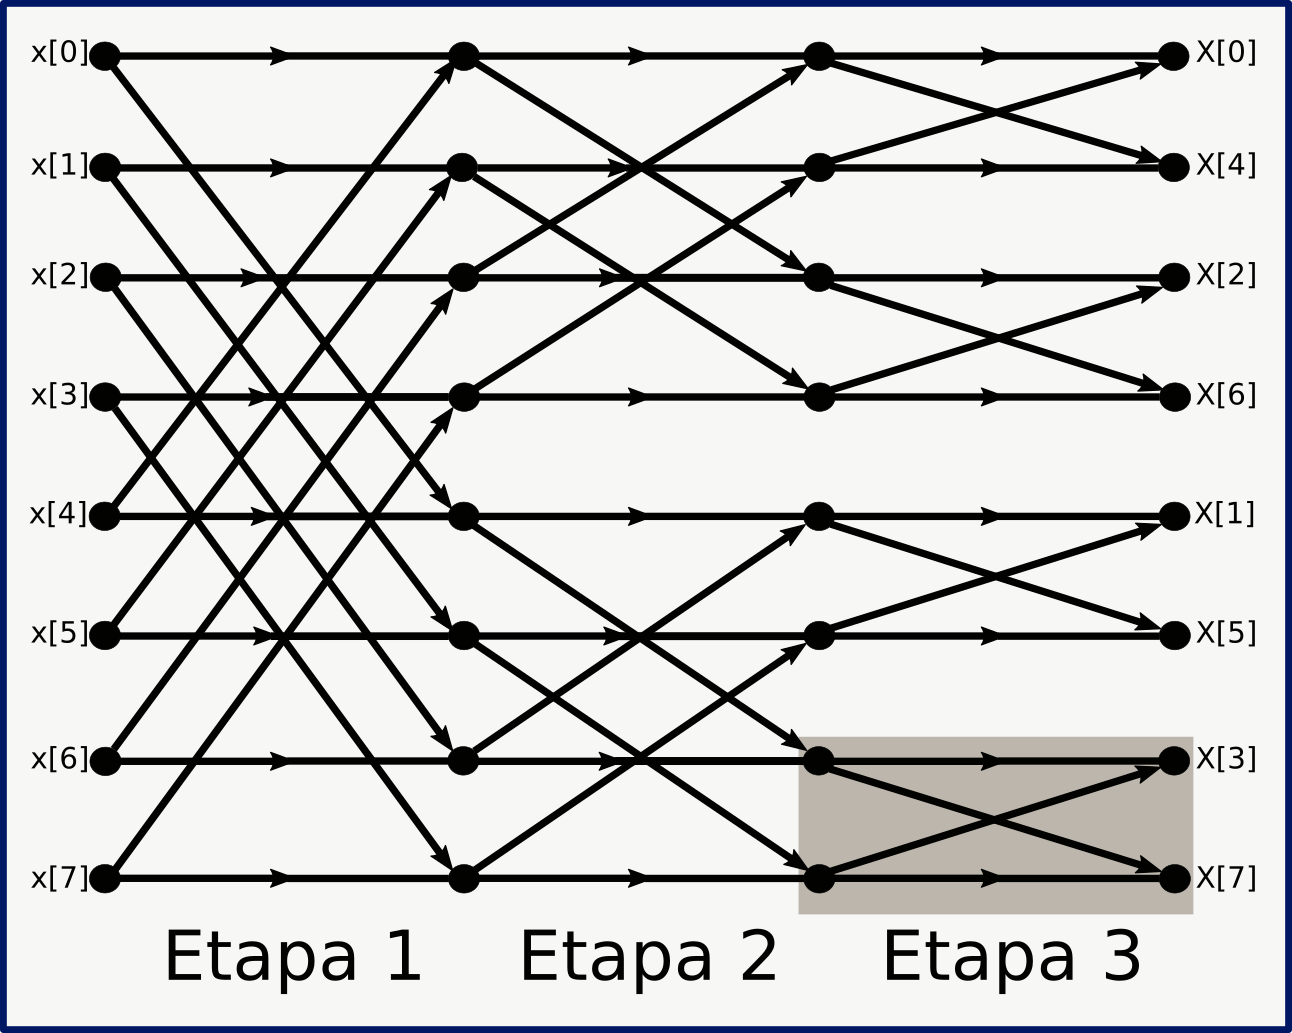
\includegraphics[width=10cm]{./figures/r2_8_diag.png}
        \caption{FFT Radix-2 de 8 puntos}
        \label{fig:r2_8_c3}
\end{figure}

Dado que los datos ingresan de a uno en la arquitectura, deben almacenarse en memoria hasta que se
tiene el dato necesario para realizar una operación aritmética. Es importante notar que en cada
etapa de cálculo aritmético se utilizan dos datos como entradas al \textit{butterfly} y se obtienen
dos datos como resultados, de los cuales uno se utiliza en la etapa siguiente y el otro se almacena en memoria.

En la arquitectura iterativa a implementar, se ejecuta en cada ciclo de \textit{clock} una operación
de una etapa, pasando a la siguiente etapa en el ciclo de \textit{clock} siguiente, de forma que al
transcurrir $\log_2(N)$ ciclos de \textit{clock} se ejecutó una operación de cada etapa volviendo a
la etapa inicial.

La figura \ref{fig:radix2blocks} muestra un diagrama en bloques de la arquitectura radix-2
iterativa. Se diferencian claramente tres partes: la memoria, la unidad aritmética, compuesta por el
\textit{butterfly} y el multiplicador, y la unidad de control. Los distintos colores de los bloques
indican si el mismo es un circuito combinacional, un circuito secuencial o una unidad de
almacenamiento. Este diagrama es a modo de esquema general y es del que se partió para el
desarrollo de la arquitectura, al final de esta sección se presenta el diagrama del
\textit{datapath} detallado con las señales de control necesarias para su funcionamiento.	


\begin{figure}[htb!]
        \centering
        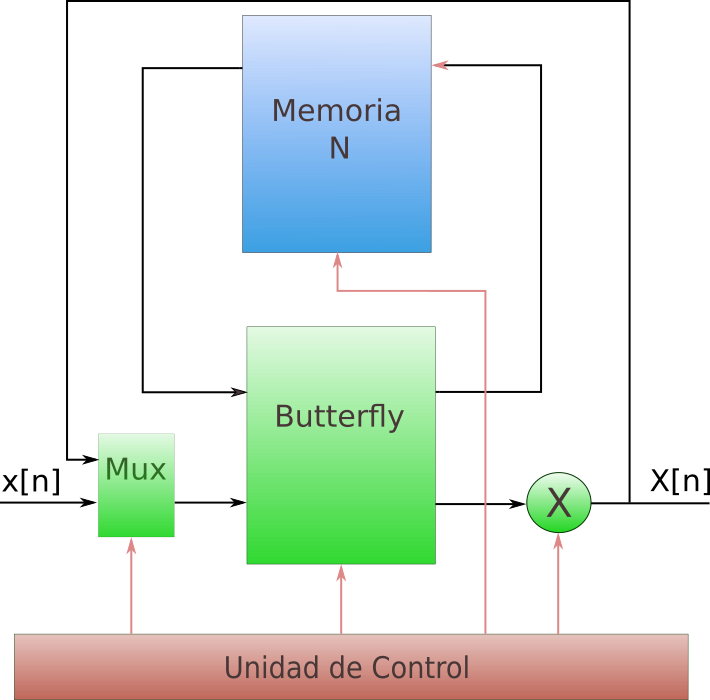
\includegraphics[width=10cm]{./figures/radix2blocks.png}
        \caption{Diagrama simplificado de la arquitectura radix-2 iterativa}
        \label{fig:radix2blocks}
\end{figure}

\subsection{Memoria} \label{sec:r2mem}

Debido al tipo de acceso a los datos se decide implementar una memoria de almacenamiento de tipo
RAM de doble acceso (\textit{dual port RAM}) permitiendo realizar simultáneamente operaciones de lectura y escritura. Las interfaces son las típicas para
esta memoria y se describen en la figura \ref{fig:dualPortRam}.

\begin{figure}[htb!]
        \centering
        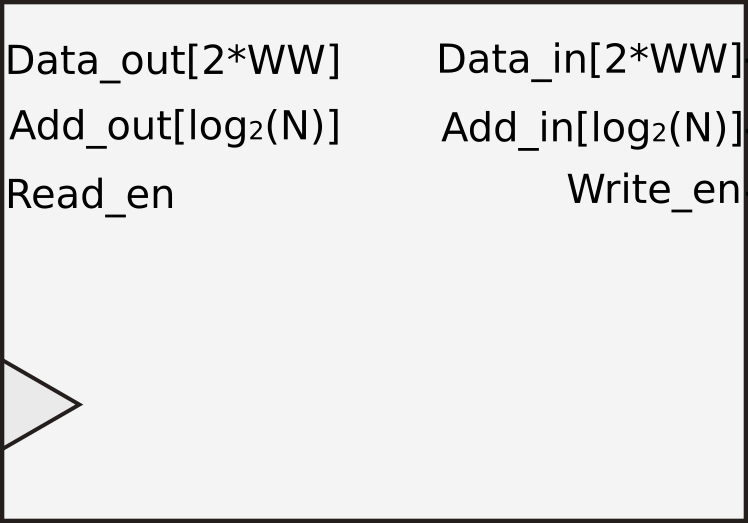
\includegraphics[width=5cm]{./figures/dportRam.png}
        \caption{Dual Port RAM}
        \label{fig:dualPortRam}
\end{figure}

En la figura \ref{fig:dualPortRam} se muestran los buses de entrada y salida indicando su tamaño
entre corchetes.
El parámetro \textit{WW} corresponde al parámetro global \textit{WORD\_WIDTH} e indica el ancho de palabra de la
arquitectura. El parámetro \textit{N} indica la cantidad de puntos para la que se configura la
arquitectura. Las variables a almecenar son complejas, por lo que se concatenan la parte real y la
imaginaria y se guardan en memoria como un único valor. De este modo el tamaño de palabra de la 
memoria es el doble del tamaño de palabra de la arquitectura, teniendo también sus buses de entrada 
y salida el doble de ancho que los demás buses de la arquitectura.

\subsection{Butterfly}

Para la arquitectura radix-2, el \textit{butterfly} debe computar con dos operandos según la
siguiente ecuación:

\begin{equation}
\begin{split}
c &= a+b \\
d &= a-b
\end{split}
\label{eq:butterf}
\end{equation}

Siendo todas las variables complejas. En la figura \ref{fig:butterfly_esq} se muestra el esquema del
bloque \textit{butterfly}, compuesto por un sumador y un restador complejos.

\begin{figure}[htb!]
        \centering
        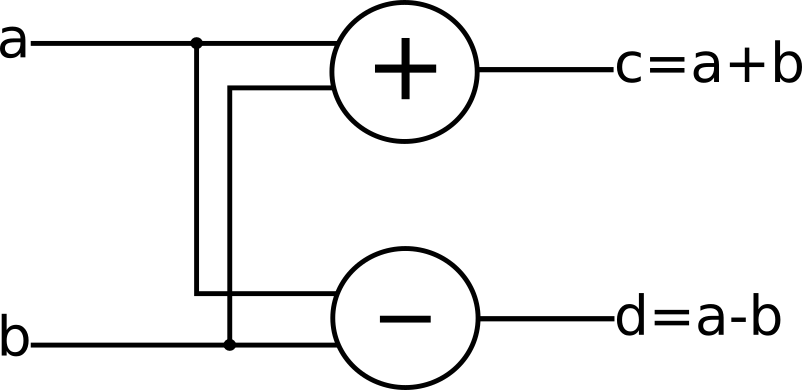
\includegraphics[width=6cm]{./figures/butterfly_esq.png}
        \caption{Esquema del bloque butterfly}
        \label{fig:butterfly_esq}
\end{figure}

\subsection{Datapath} \label{sec:datapath}

En la figura \ref{fig:datapath} se muestra el \textit{datapath} de la arquitectura radix-2. Se muestra el
butterfly como un sumador y un restador, y un multiplicador genérico que puede ser implementado como
un procesador cordic o como un multiplicador complejo. Dado que en las etapas intermedias y en la
etapa final se debe operar con un dato de la etapa anterior se coloca un registro (\textit{delay
register}) donde se almacena ese dato durante un ciclo de clock para ser utilizado en la etapa siguiente. 
A la salida se le coloca un registro similar para facilitar la
sincronización con otros elementos del entorno de la arquitectura.

\begin{figure}[htb!]
        \centering
        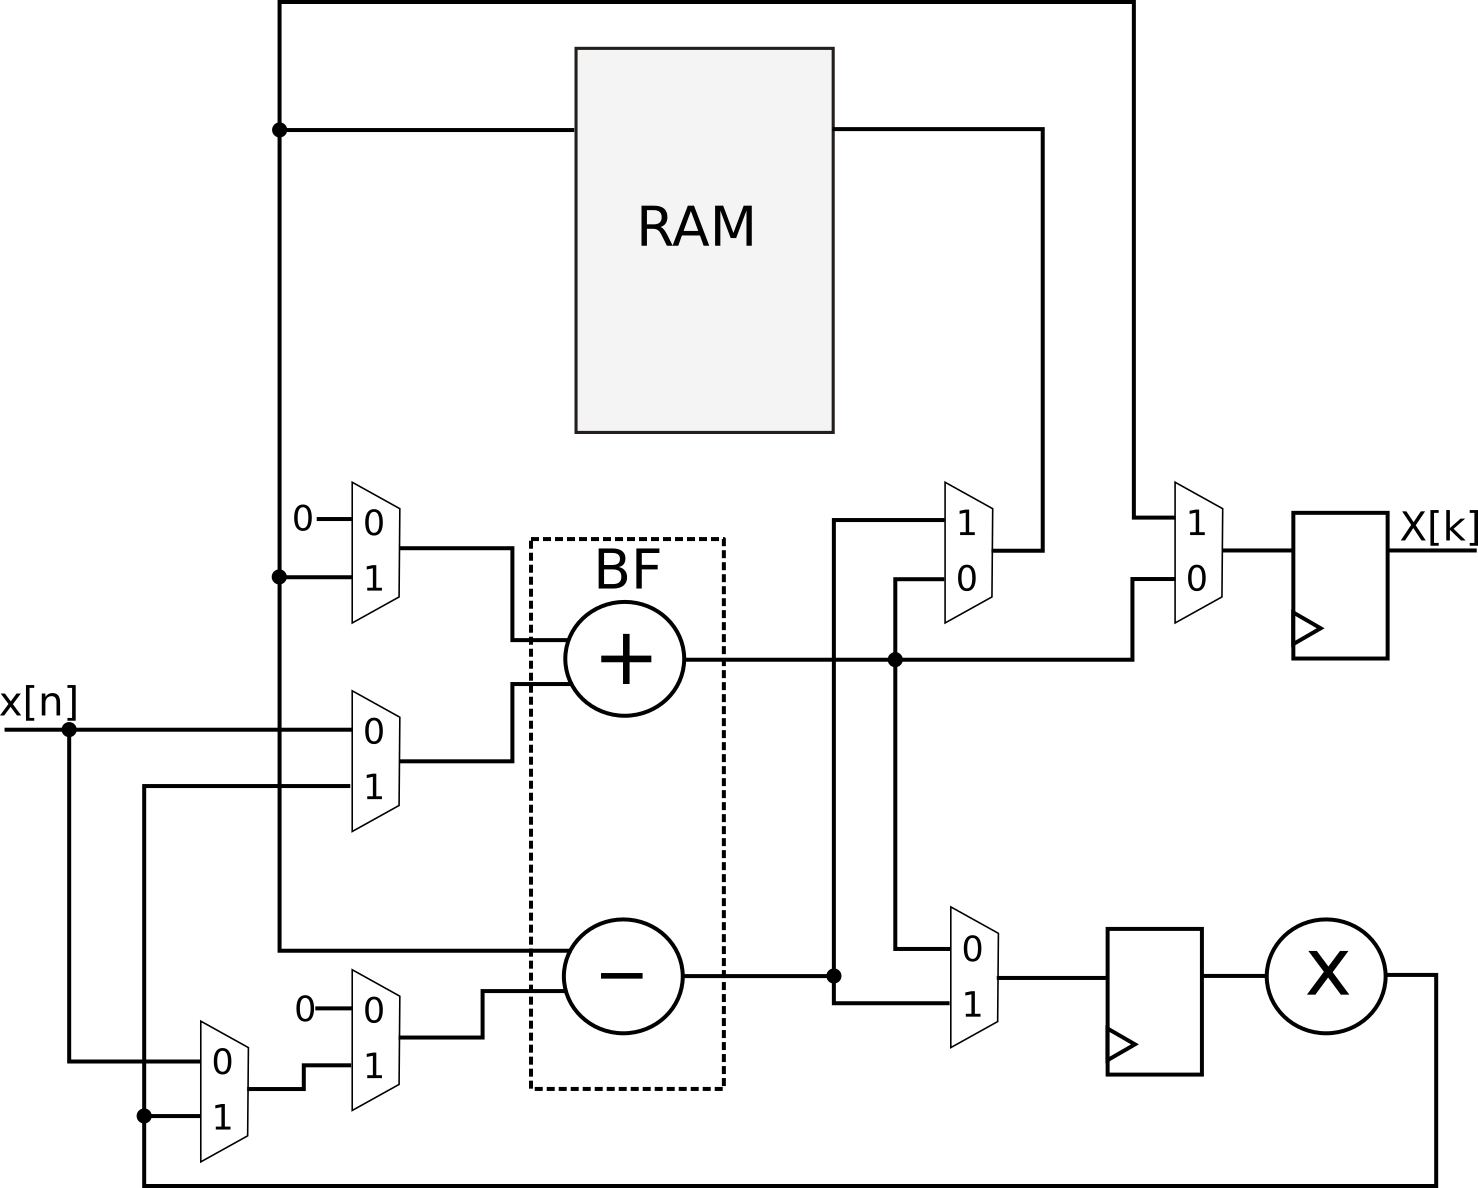
\includegraphics[width=10cm]{./figures/datapath.png}
        \caption{Esquema del datapath de la arquitectura radix-2}
        \label{fig:datapath}
\end{figure}

A través de los multiplexores se configura el \textit{datapath} de acuerdo a la etapa en que se encuentra y
el tipo de operación a realizar. De la figura \ref{fig:radix2blocks} se deduce que en cada fase de
cómputo se puede realizar una de dos acciones posibles, entra un dato a memoria mientras que otro dato 
sale de memoria hacia el multiplicador o se opera en el \textit{butterfly} con un dato de memoria y otro dato que viene
de la entrada o de la etapa anterior.

En la figura \ref{fig:datapathMem} se muestran las tres configuraciones posibles del \textit{datapath} para
las operaciones de tranferencias de datos en memoria. En este tipo de operación se lee un dato de
memoria y se envía al multiplicador para realizar el producto por el \textit{twiddle fator} o hacia
la salida y se escribe un dato en memoria proveniente de la entrada o de la etapa anterior a través
del \textit{delay register}.

% \begin{figure}[htb!]
%         \centering
%         \subfigure[Etapa
%         inicial]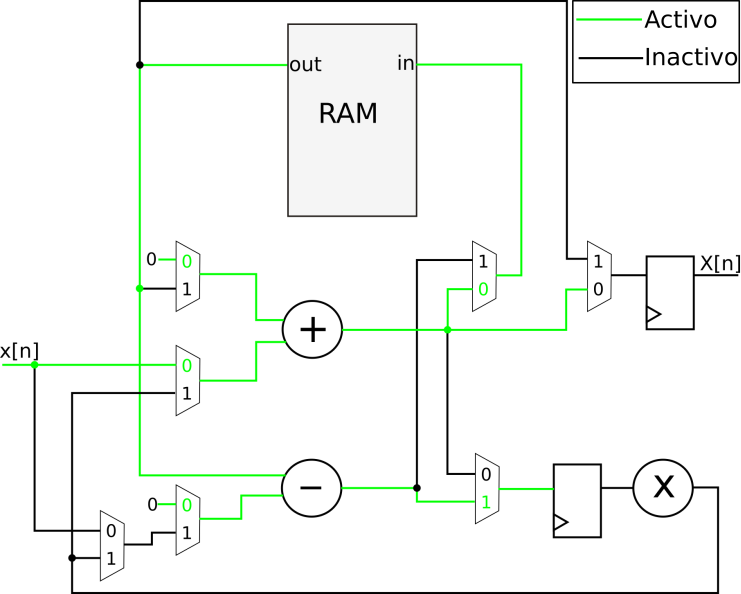
\includegraphics[width=7cm]{./figures/datapath_mem1.png}}
%         \subfigure[Etapas
%         intermedias]}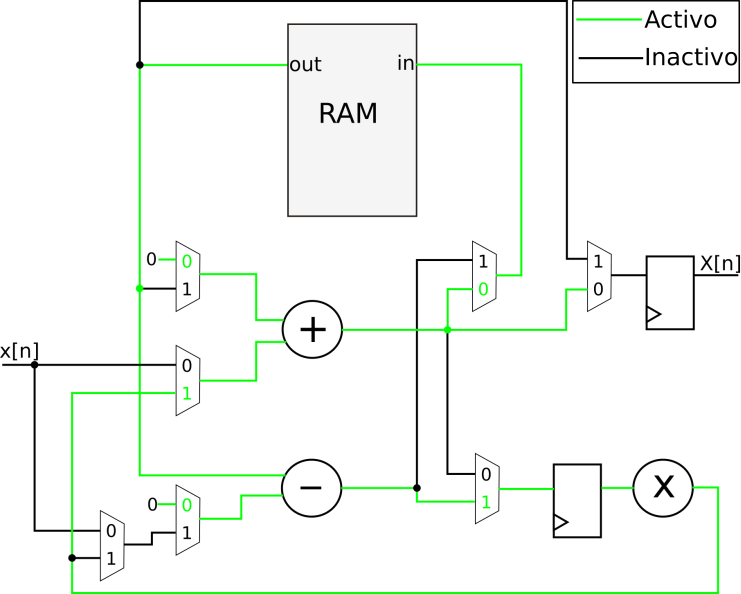
\includegraphics[width=7cm]{./figures/datapath_memint.png}}
%         \subfigure[Etapa
%         final]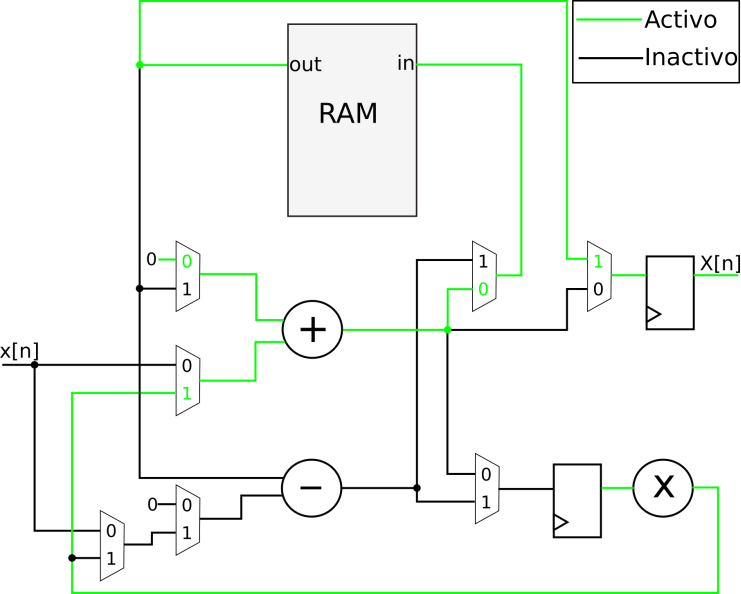
\includegraphics[width=7cm]{./figures/datapath_memf.png}}
%         \caption{Datapath para operaciones de transferencia en memoria}
%         \label{fig:datapathMem}
% \end{figure}

\begin{figure}[htb!]
        \centering
        \begin{subfigure}{\columnwidth}\centering
        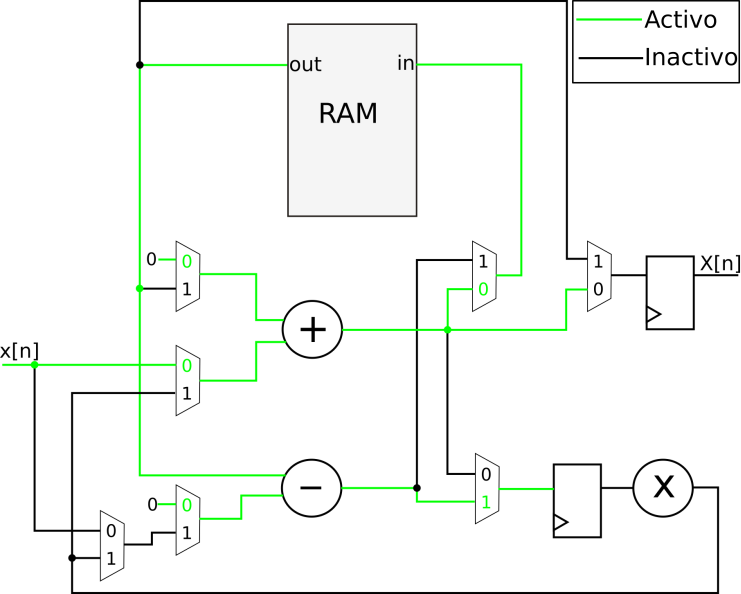
\includegraphics[width=7cm]{./figures/datapath_mem1.png}
        \caption{Etapa inicial}
        \end{subfigure}
        \begin{subfigure}{\columnwidth}\centering
        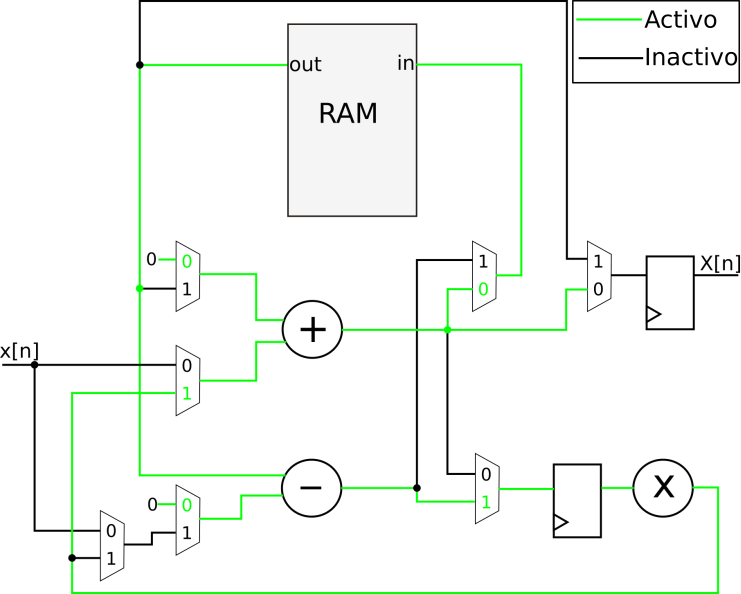
\includegraphics[width=7cm]{./figures/datapath_memint.png}
        \caption{Etapas intermedias}
        \end{subfigure}
        \begin{subfigure}{\columnwidth}\centering
        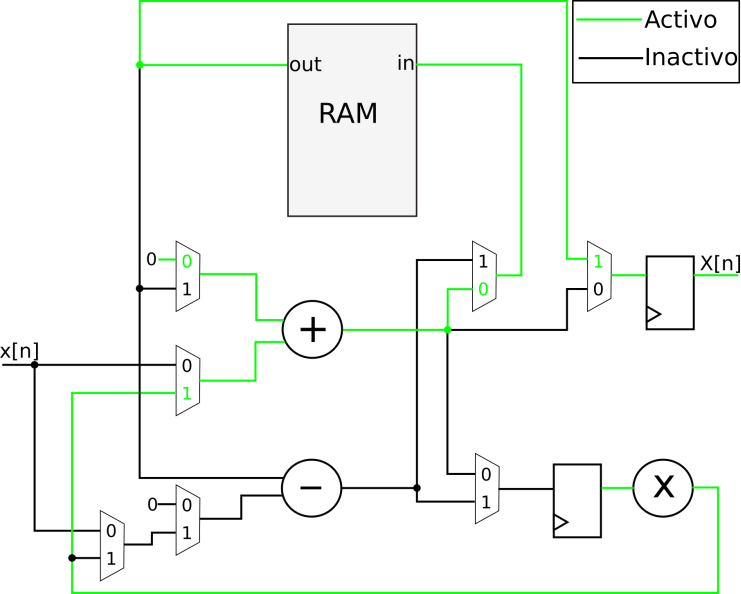
\includegraphics[width=7cm]{./figures/datapath_memf.png}
        \caption{Etapa final}
        \end{subfigure}
        \caption{Datapath para operaciones de transferencia en memoria}
        \label{fig:datapathMem}
\end{figure}

En la figura \ref{fig:datapathBut} se muestran los posibles \textit{datapath} para las operaciones en el
butterfly. Dependiendo de si la etapa es la etapa inicial o una intermedia uno de los operandos será
la entrada de la arquitectura o un dato de la entrada anterior almacenado en el \textit{delay
register} y el otro operando provendrá de la memoria. La salida del restador del butterfly se envía
directamente a memoria y la salida del sumador puede ir al \textit{delay register} para ser
utilizado en la etapa siguiente o puede ser direccionado a la salida de la arquitectura dependiendo
de si la etapa es intermedia o es la etapa de salida.

\begin{figure}[htb!]
        \centering
        \begin{subfigure}{\columnwidth}\centering
        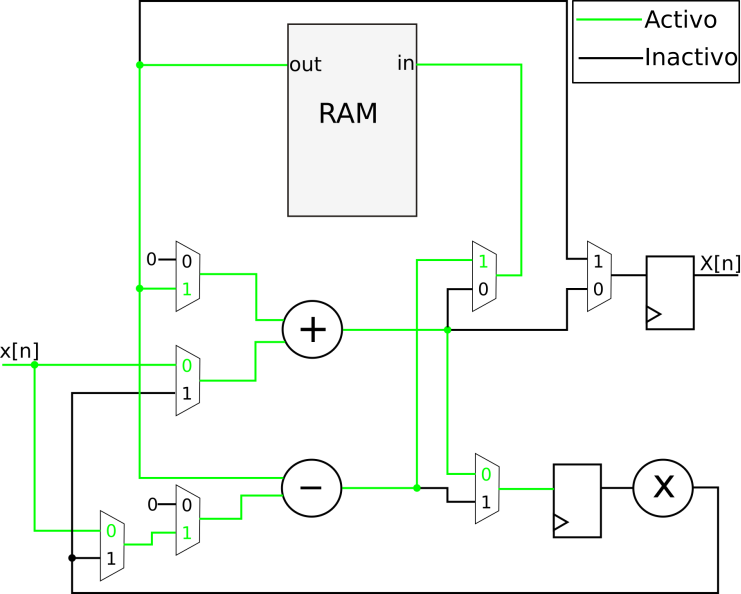
\includegraphics[width=7cm]{./figures/datapath_but1.png}
        \caption{Etapa inicial}
        \end{subfigure}
        \begin{subfigure}{\columnwidth}\centering
        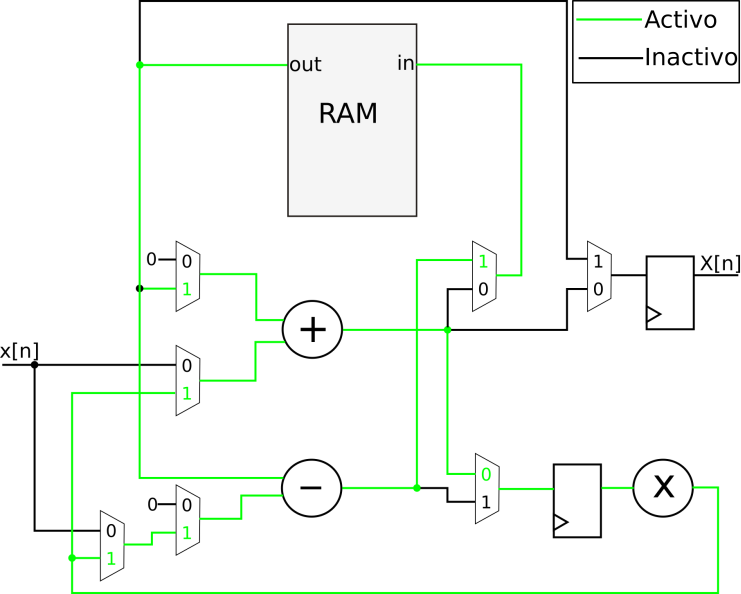
\includegraphics[width=7cm]{./figures/datapath_butint.png}
        \caption{Etapas intermedias}
        \end{subfigure}
        \begin{subfigure}{\columnwidth}\centering
        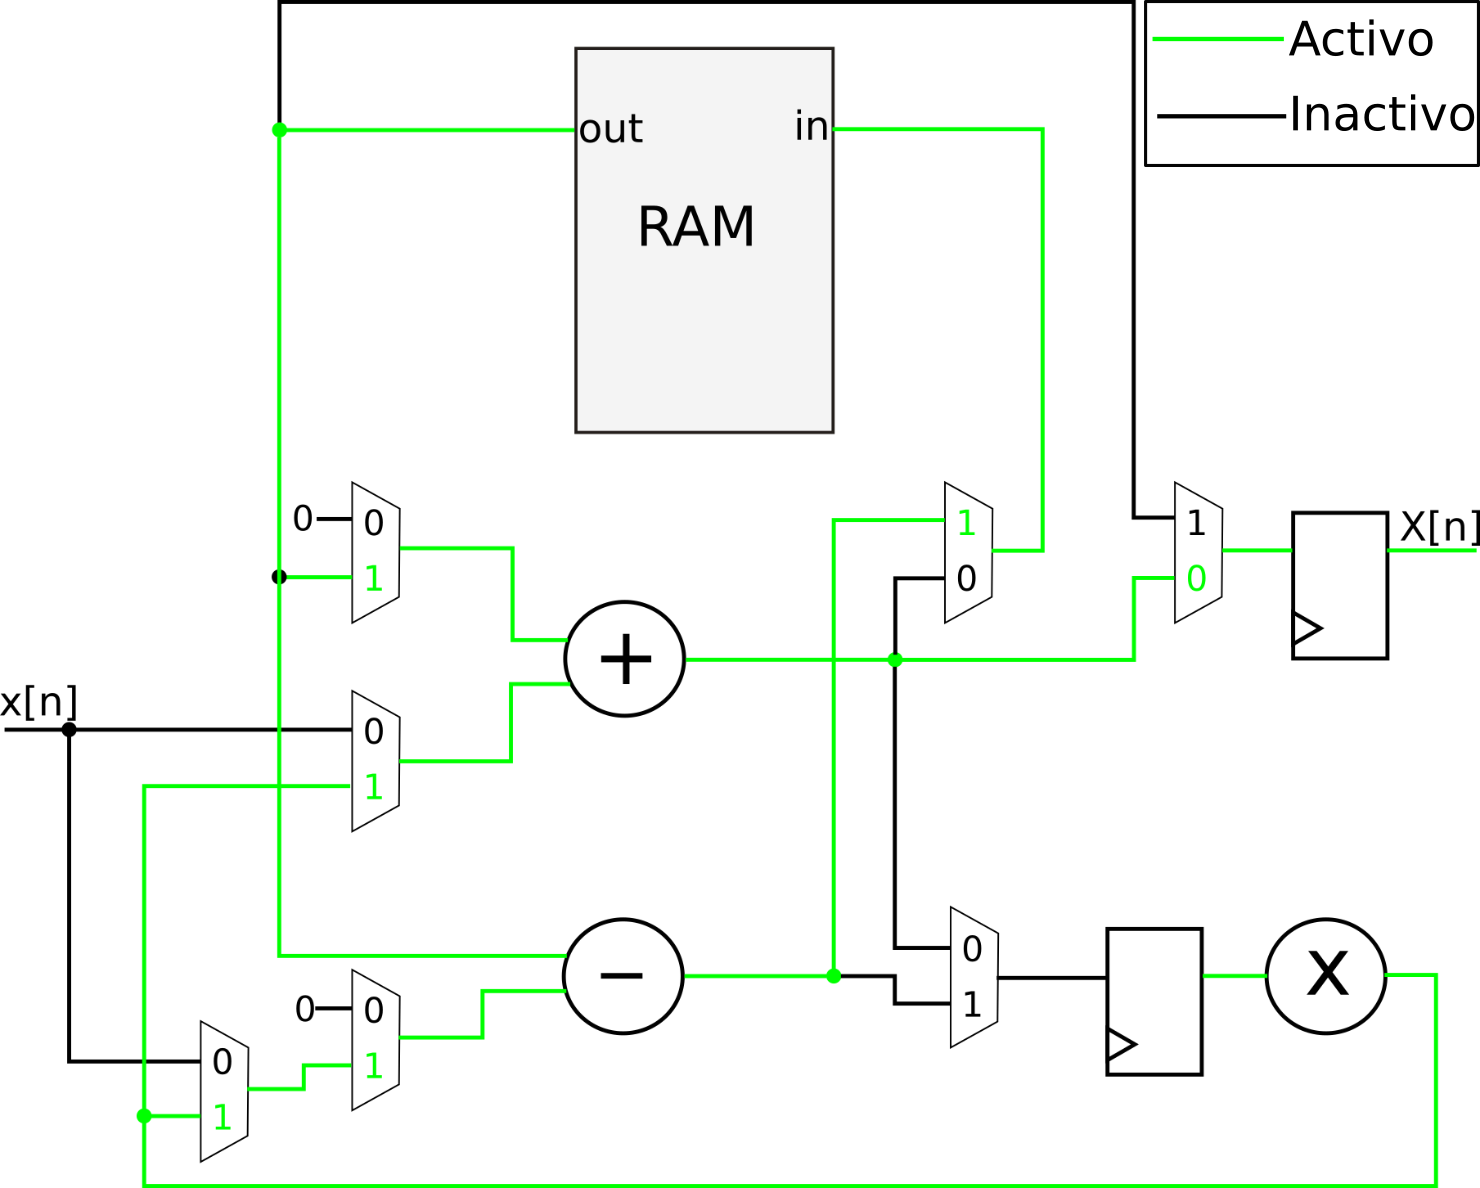
\includegraphics[width=7cm]{./figures/datapath_butf.png}
        \caption{Etapa final}
        \end{subfigure}
        \caption{Datapath para operaciones en butterfly}
        \label{fig:datapathBut}
\end{figure}

\subsection{Unidad de control}

La unidad de control debe contener la máquina de estados que controla el funcionamiento de la
arquitectura, la configuración del \textit{datapath} en cada ciclo de \textit{clock}, el manejo de
la memoria donde se almacenan los valores de cálculo y la generación de los \textit{twiddle factors}
para el multiplicador.

Teniendo en cuenta que ingresa a la arquitectura un punto nuevo cada $log_2(N)$ ciclos de
\textit{clock} se utiliza un contador de etapas de longitud $log_2(log_2(N))$ para identificar la
etapa del cómputo de la fft en que se encuentra la arquitectura. El desborde de este contador
alimenta otro contador de longitud  $log_2(N)$ que cuenta la cantidad de puntos que han ingresado a
la arquitectura. Con estos dos contadores se lleva el control de la máquina de estados, que controla
la configuración del \textit{datapath} y la memoria, y la generación de los \textit{twiddle
factors}.

En la subsección \ref{sec:datapath} se describieron las distintas configuraciones del \textit{datapath}, que
deben ser gestionadas por la unidad de control de acuerdo a la etapa en que se encuentra la
arquitectura y si debe realizar una transferencia a memoria o un cálculo en el butterfly. Tomando
como ejemplo la radix-2 de $8$ puntos de la figura \ref{fig:r2_8_c3}, se ve que en la primera etapa se debe esperar la llegada del quinto punto para realizar una operación en el \textit{butterfly}, por lo que las primeras cuatro operaciones de esa etapa serán trasnferencias de los puntos a memoria y las últimas cuatro serán operaciones en el
\textit{butterfly}. Para la segunda etapa la secuencia será de dos operaciones de transferencia a
memoria y dos de operaciones aritméticas. Y para la última etapa serán operaciones de transferencia
a memoria y aritméticas alternadas de a una. Entonces para una cierta etapa $i \epsilon \{0 \leq i
\leq log_2(N)-1\}$ la cantidad de operaciones consecutivas de cada tipo está dada por

\begin{equation}
log_2(\frac{N}{i+1})
\label{eq:etapas}
\end{equation}

Para determinar si se debe realizar una transferencia a memoria o una operación aritmética, se
utiliza un solo bit del contador de puntos. El bit a evaluar se determina en función de la etapa que
se está procesando, a través del \textit{stg\_ctr}, el contador de etapas, de $\log_2(\log_2(N))$
bits, como se muestra en la figura \ref{fig:r2conts}.

% Para determinar \ref{eq:etapas} en cada ciclo de \textit{clock} se observa en el contador de puntos
% el bit dado por $log_2(N) - contador_{etapas} - 1$, entonces en la primer etapa (contador de etapas
% en cero) se evalúa el bit más alto del contador de puntos, y así sucesivamente hasta evaluar el bit
% más bajo del contador de puntos en la última etapa (donde $contador_{etapas} = log_2(N) - 1$). En
% la figura \ref{fig:r2conts} se muestra un esquema de la selección del bit del contador de puntos
% de acuerdo al valor del $contador_{etapas}$ para una arquitectura de 256 puntos. De esta forma si el
% bit del contador de puntos correspondiente a una etapa vale $'0'$ se realiza una trasnferencia a
% memoria, y si vale $'1'$ se realiza una operación en el \textit{butterfly}.

\begin{figure}[htb!]
        \centering
        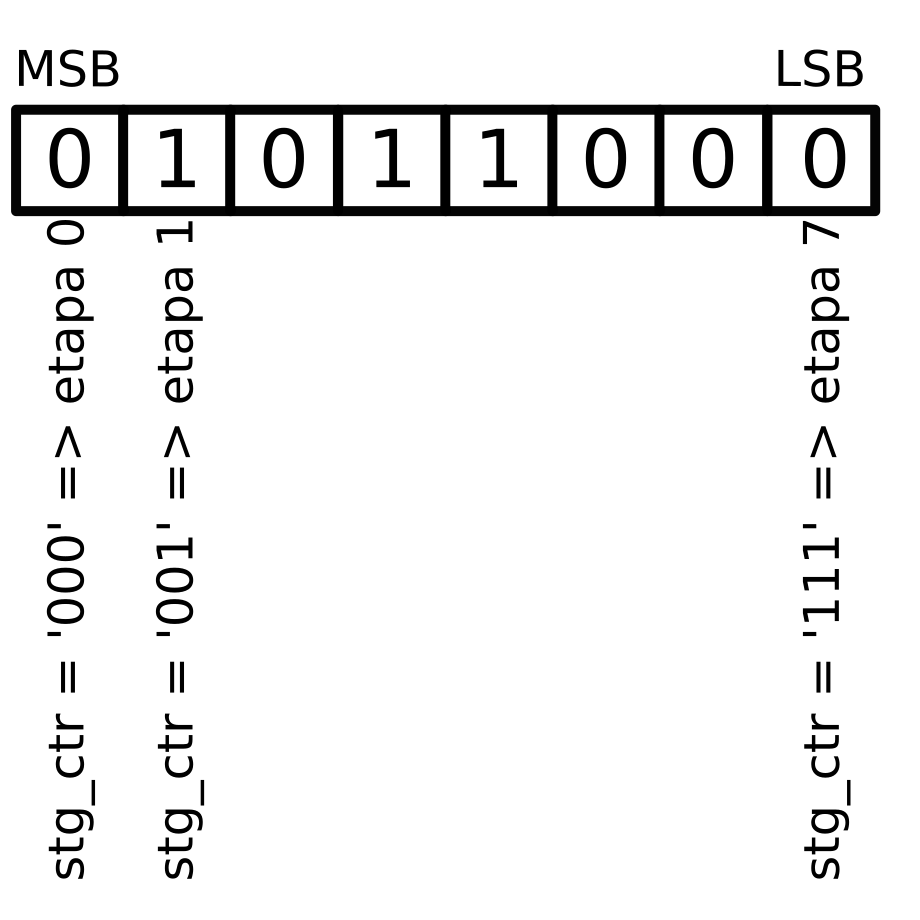
\includegraphics[width=6cm]{./figures/r2conts.png}
        \caption{Selección del bit del contador de puntos a evaluar}
        \label{fig:r2conts}
\end{figure}


\subsubsection{Máquinas de estados}

La unidad de control se compone de una máquina de estados principal que controla la inicialización
de los módulos de la arquitectura y una máquina de estados operativa que controla la
configuración del \textit{datapath} dependiendo de la operación que se debe realizar.
En la figura \ref{fig:mainSMr2} se muestran los estados y transiciones de la máquina de estados
principal.

\begin{figure}[htb!]
        \centering
        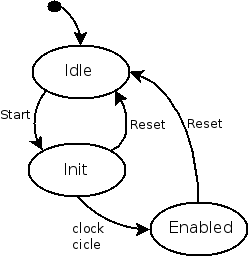
\includegraphics[width=6cm]{./figures/SMr2gen.png}
        \caption{Estados de la máquina de estados principial}
        \label{fig:mainSMr2}
\end{figure}

El estado inicial de la arquitectura es el estado
\textit{Idle}, donde permanece aguardando una señal para iniciar el proceso. La señal de
\textit{start} tiene la finalidad de sincronizar la arquitectura con el entorno al que está conectada, y lleva la
máquina de estados al estado \textit{Init} donde se inicializan los registros a valores conocidos y
se configura el \textit{datapath} para comenzar el procesamiento, leyendo ya el primer dato de la
entrada. Un ciclo de \textit{clock} después la máquina de estados pasa directamente al estado \textit{Enabled} 
donde se realiza el procesamiento. Dentro de
este estado se encuentra la máquina de estados operativa que se describe a continuación.

\begin{figure}[htb!]
        \centering
        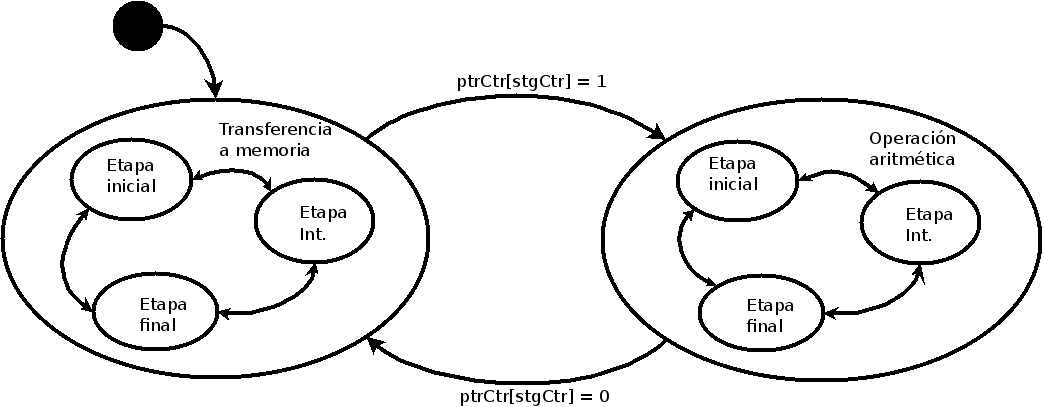
\includegraphics[width=13cm]{./figures/SMr2op.png}
        \caption{Máquina de estados operativa para modo \textit{enabled}}
        \label{fig:opSMr2}
\end{figure}

En la figura \ref{fig:opSMr2} se observan los estados y transiciones de la máquina de estados
que controla la configuración del \textit{datapath} de acuerdo al tipo de operación a
realizar.
En cada uno de los estados principales funciona una máquina de estados secundaria que realiza
ajustes menores de acuerdo a si la etapa actual es la etapa inicial, una intermedia o la etapa final. $ptrCtr[stgCtr]$ hace
referencia al bit del contador de puntos correspondiente al valor del contador de etapas, de
acuerdo a lo expuesto en la figura \ref{fig:r2conts}.\\
Esta máquina de estados controla además la señal de habilitación de escalamiento para la etapa
actual de acuerdo al vector de escalamiento de entrada a la arquitectura. También controla, a través
del contador de puntos y el de etapas, las señales de \textit{handshaking} de salida, indicando si
el dato de salida es un dato válido, señal \textit{data\_valid} y las señales que indican si es el
punto inicial (\textit{soo}) o final (\textit{done})del cómputo actual.

\subsubsection{Control de la memoria}

Dado que el algoritmo radix-2 permite el alojamiento \textit{data in place} el manejo de la memoria
es relativamente sencillo. 
En cada operación de una etapa se realiza siempre una escritura de datos, ya sea un dato entrante a
la etapa (nuevo o de una etapa anterior) o del resultado de una operación aritmética. En cambio solo
se realizan lecturas de memoria en las etapas intermedias y en la última.
Al ser un algoritmo \textit{data in place} las direcciones de memoria tanto de escritura como de
lectura se calculan utilizando el contador de puntos, ya que cada en cada posición de memoria
donde se alojaba un dato utilizado para una operación aritmética se alojará el resultado
correspondiente a esa operación una vez realizada. Entonces en una etapa determinada se lee la
posición de memoria $k$, se realiza un cálculo con ese dato, y se guarda nuevamente en la posición
$k$ el resultado del cálculo.
Al acceder continuamente a la memoria tanto en modo escritura como lectura, las señales
correspondientes de control de la memoria están siempre en modo habilitación.

\subsubsection{Control del datapath}

El control del \textit{datapath} se realiza mediante los multiplexores que se ven en la figura
\ref{fig:datapath} a través de señales digitales. En cada ciclo de \textit{clock}, de acuerdo a la máquina de
estados que decide en que etapa se encuentra el algoritmo y dependiendo de la operación a realizar
se configuran los multiplexores para conformar el datapath según las figuras \ref{fig:datapathMem}
y \ref{fig:datapathBut}.

\subsection{Integración de la unidad de control}

En la figura \ref{fig:datapathmem} se muestra el \textit{datapath} de la figura \ref{fig:datapath} con el
agregado de las señales de control sobre cada módulo. No se muestra la unidad de control en forma
explícita para mantener la claridad del esquema. En el bloque butterfly además del
sumador/restador se integra el algoritmo de escalamiento que se describe en la sección
\ref{sec:secEscal}.

\begin{figure}[htb!]
        \centering
        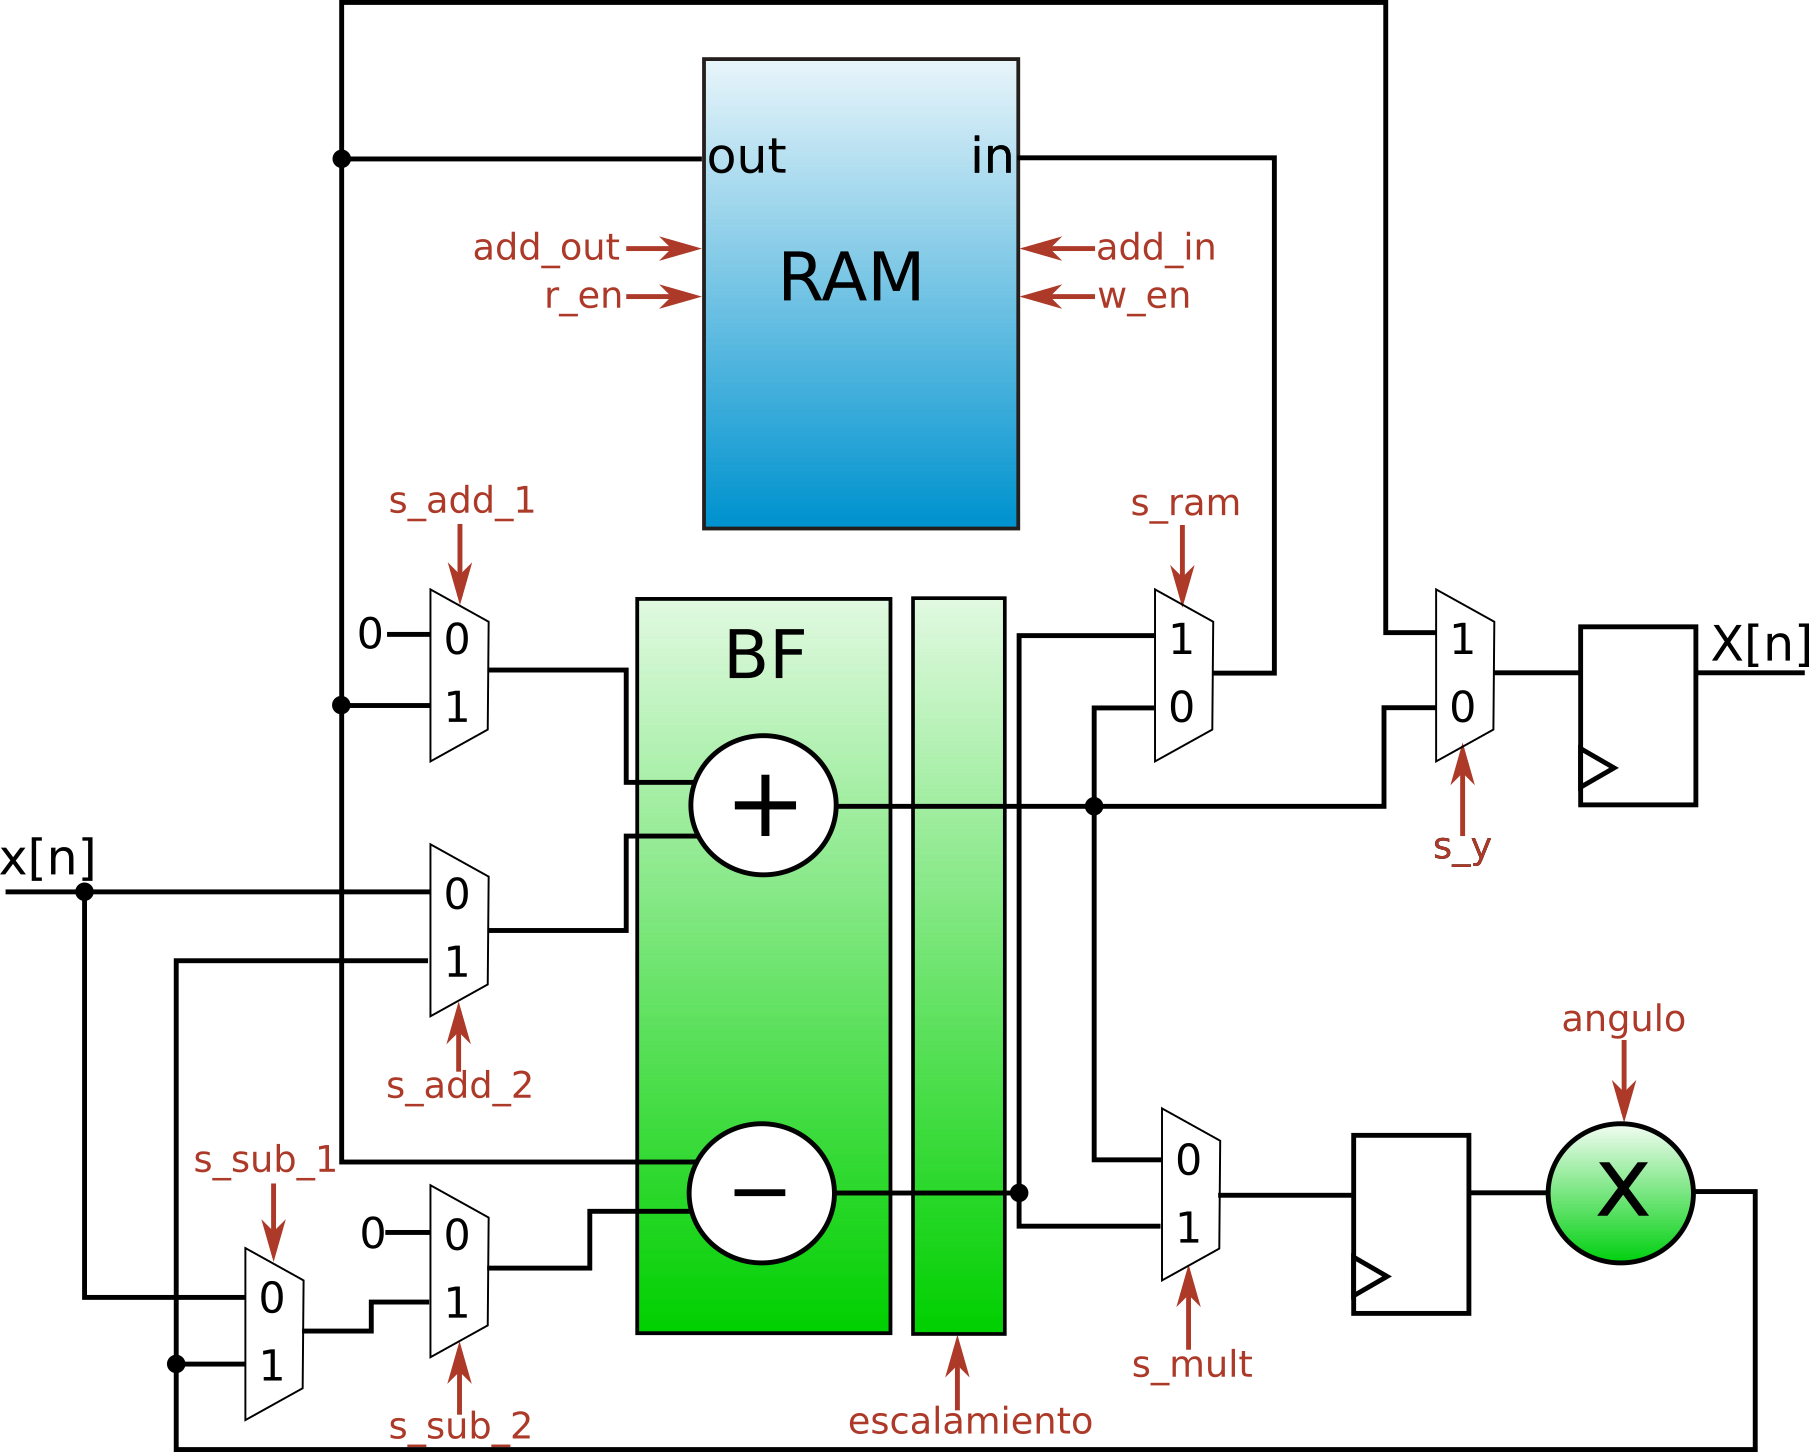
\includegraphics[width=12cm]{./figures/datapathMem.png}
        \caption{Datapath con las señales de control}
        \label{fig:datapathmem}
\end{figure}

En la figura \ref{fig:datapathmem} se muestran las siguientes señales de control (se indica entre
paréntesis el tamaño de las señales en caso que sea mayor a 1):

\begin{itemize}
  \item \textbf{add\_in} ($log_2(N)$) \textit{address in}, dirección de memoria donde se escribirá
  el dato
  \item \textbf{w\_en} \textit{write enable}, señal de habilitación de escritura en memoria
  \item \textbf{add\_out} ($log_2(N)$) \textit{address out}, dirección de memoria desde la que leerá
  el dato
  \item \textbf{r\_en} \textit{read enable}, señal de habilitacón de lectura de memoria
  \item \textbf{s\_add\_1} señal de control del multiplexor de la entrada $1$ del sumador
  \item \textbf{s\_add\_2} señal de control del multiplexor de la entrada $2$ del sumador
  \item \textbf{s\_sub\_1} señal de control del multiplexor de tipo de entrada del restador
  \item \textbf{s\_sub\_2} señal de control del multiplexor de entrada del restador
  \item \textbf{s\_mult} señal de control del multiplexor de entrada del multiplicador
  \item \textbf{s\_ram} señal de control del multiplexor de entrada de la memoria RAM
  \item \textbf{s\_y} señal de control del multiplexor de origen de la salida
  \item \textbf{angulo} ($N+1$) angulo de rotación para el multiplicador, ya sea cordic o
  multiplicador complejo.
  \item \textbf{escalamiento} señal de indicación de que en la etapa actual se realiza
  redondeo/truncamiento. 
\end{itemize}

\section{Arquitectura Radix-4}
\subsection{Descripción general}

El algoritmo Radix-4 descompone el cómputo de una DFT de N puntos en $\nu$ DFTs de 4 puntos cada
una de forma que $N = 4^\nu$.\\ Partiendo de la definición de DFT:

\begin{equation}
\begin{split}
 X_k &= \sum\limits_{n=0}^{N-1}x_n W_N^{kn} \\
 &= \sum\limits_{n=0}^{\frac{N}{4}-1}x_n W_N^{kn} + \sum\limits_{n=\frac{N}{4}}^{\frac{N}{2}-1}x_n
 W_N^{kn} + \sum\limits_{n=\frac{N}{2}}^{\frac{3N}{4}-1}x_n W_N^{kn} +
 \sum\limits_{n=\frac{3N}{4}}^{N-1}x_n W_N^{kn} \\
 &= \sum\limits_{n=0}^{\frac{N}{4}-1}x_n W_N^{kn} +
 \sum\limits_{n=0}^{\frac{N}{4}-1}x_{n+\frac{N}{4}} W_N^{k(n+\frac{N}{4})} +
 \sum\limits_{n=0}^{\frac{N}{4}-1}x_{n+\frac{N}{2}} W_N^{k(n+\frac{N}{2})} + 
 \sum\limits_{n=0}^{\frac{N}{4}-1}x_{n+\frac{3N}{4}} W_N^{k(n+\frac{3N}{4})} \\
 &= \sum\limits_{n=0}^{\frac{N}{4}-1}x_n W_N^{kn} +
 W_4^k \sum\limits_{n=0}^{\frac{N}{4}-1}x_{n+\frac{N}{4}} W_N^{kn} +
 W_4^{2k} \sum\limits_{n=0}^{\frac{N}{4}-1}x_{n+\frac{N}{2}} W_N^{kn} + 
 W_4^{3k}\sum\limits_{n=0}^{\frac{N}{4}-1}x_{n+\frac{3N}{4}} W_N^{kn} \\
 &= \sum\limits_{n=0}^{\frac{N}{4}-1}(x_n + x_{n+\frac{N}{4}} W_4^k + x_{n+\frac{N}{2}} W_4^{2k} + 
 x_{n+\frac{3N}{4}} W_4^{3k}) W_N^{kn}
\end{split}
\label{eq:radix4_1}
\end{equation}

El resultado final en (\ref{eq:radix4_1}) se puede descomponer en cuatro subproblemas para los casos
$4k$, $4k+1$, $4k+2$ y $4k+3$ dando lugar a:

\begin{equation}
\begin{split}
Y_k = X_{4k} &= \sum\limits_{n=0}^{\frac{N}{4}-1}(x_n + x_{n+\frac{N}{4}} W_4^{4k} +
x_{n+\frac{N}{2}} W_4^{2*4k} + x_{n+\frac{3N}{4}} W_4^{3*4k}) W_N^{4kn} \\
&= \sum\limits_{n=0}^{\frac{N}{4}-1}(x_n + x_{n+\frac{N}{4}} + x_{n+\frac{N}{2}} +
x_{n+\frac{3N}{4}}) W_{\frac{N}{4}}^{kn} \\
&= \sum\limits_{n=0}^{\frac{N}{4}-1} y_k W_{\frac{N}{4}}^{kn}, \qquad k = 0,1,\ldots,\frac{N}{4}-1
\end{split}
\label{eq:radix4_Y}
\end{equation}

\begin{equation}
\begin{split}
Z_k = X_{4k+1} &= \sum\limits_{n=0}^{\frac{N}{4}-1}(x_n + x_{n+\frac{N}{4}} W_4^{4k+1} +
x_{n+\frac{N}{2}} W_4^{2*(4k+1)} + x_{n+\frac{3N}{4}} W_4^{3*(4k+1)}) W_N^{(4k+1)n} \\
&= \sum\limits_{n=0}^{\frac{N}{4}-1}((x_n - x_{n+\frac{N}{2}}) -j (x_{n+\frac{N}{4}}
-x_{n+\frac{3N}{4}})) W_N^{k} W_{\frac{N}{4}}^{kn} \\
&= \sum\limits_{n=0}^{\frac{N}{4}-1} z_k W_{\frac{N}{4}}^{kn}, \qquad k = 0,1,\ldots,\frac{N}{4}-1
\end{split}
\label{eq:radix4_Z}
\end{equation}

\begin{equation}
\begin{split}
G_k = X_{4k+2} &= \sum\limits_{n=0}^{\frac{N}{4}-1}(x_n + x_{n+\frac{N}{4}} W_4^{4k+2} +
x_{n+\frac{N}{2}} W_4^{2*(4k+2)} + x_{n+\frac{3N}{4}} W_4^{3*(4k+2)}) W_N^{(4k+2)n} \\
&= \sum\limits_{n=0}^{\frac{N}{4}-1}((x_n + x_{n+\frac{N}{2}}) - (x_{n+\frac{N}{4}}
+ x_{n+\frac{3N}{4}})) W_N^{2k} W_{\frac{N}{4}}^{kn} \\
&= \sum\limits_{n=0}^{\frac{N}{4}-1} g_k W_{\frac{N}{4}}^{kn}, \qquad k = 0,1,\ldots,\frac{N}{4}-1
\end{split}
\label{eq:radix4_G}
\end{equation}

\begin{equation}
\begin{split}
H_k = X_{4k+3} &= \sum\limits_{n=0}^{\frac{N}{4}-1}(x_n + x_{n+\frac{N}{4}} W_4^{4k+3} +
x_{n+\frac{N}{2}} W_4^{2*(4k+3)} + x_{n+\frac{3N}{4}} W_4^{3*(4k+3)}) W_N^{(4k+3)n} \\
&= \sum\limits_{n=0}^{\frac{N}{4}-1}((x_n - x_{n+\frac{N}{2}}) +j (x_{n+\frac{N}{4}}
- x_{n+\frac{3N}{4}})) W_N^{3k} W_{\frac{N}{4}}^{kn} \\
&= \sum\limits_{n=0}^{\frac{N}{4}-1} h_k W_{\frac{N}{4}}^{kn}, \qquad k = 0,1,\ldots,\frac{N}{4}-1
\end{split}
\label{eq:radix4_H}
\end{equation}

Entonces, la unidad aritmética de la arquitectura radix-4 debe procesar cuatro puntos, $x_n$,
$x_{n+\frac{l}{4}}$, $x_{n+\frac{l}{2}}$ y $x_{n+\frac{l}{4}}$, obteniéndose como resultado:

\begin{equation}
y_n = (x_n + x_{n+\frac{l}{4}} + x_{n+\frac{l}{2}} + x_{n+\frac{3l}{4}}) \qquad k =
0,1,\ldots,\frac{N}{4}-1
\label{eq:radix4_suby}
\end{equation}

\begin{equation}
z_n = ((x_n - x_{n+\frac{l}{2}}) -j (x_{n+\frac{l}{4}}
-x_{n+\frac{3l}{4}})) W_N^{k} \qquad k = 0,1,\ldots,\frac{N}{4}-1
\label{eq:radix4_subz}
\end{equation}

\begin{equation}
g_n = ((x_n + x_{n+\frac{l}{2}}) - (x_{n+\frac{l}{4}}
+ x_{n+\frac{3l}{4}})) W_N^{2k} \qquad k = 0,1,\ldots,\frac{N}{4}-1
\label{eq:radix4_subg}
\end{equation}

\begin{equation}
h_n = ((x_n - x_{n+\frac{l}{2}}) +j (x_{n+\frac{l}{4}} - x_{n+\frac{3l}{4}})) W_N^{3k} \qquad k = 0,1,\ldots,\frac{N}{4}-1
\label{eq:radix4_subh}
\end{equation}

donde $l$ depende de la etapa del cómputo a la que pertenece el cálculo y se define como sigue

\begin{equation}
\begin{split}
l_1 &= N \\
l_2 &= \log_4(N) \\
l_3 &= \log_4(\log_4(N))\\ 
..&.\\
l_\nu &= 4
\end{split}
\label{eq:radix_4_arit_l}
\end{equation}

donde $l_i$ corresponde a la etapa i-ésima de una FFT de $N=4^\nu$ puntos.

En la figura \ref{fig:r4_diag} se muestra un esquema del cómputo de una radix-4 para 16 puntos,
similar al esquema de la radix-2 de la figura \ref{fig:r2_8_c3}, donde se ve el cómputo aritmético
utilizando cuatro puntos como entrada y obteniendo cuatro puntos como salida.

\begin{figure}[htb!]
        \centering
        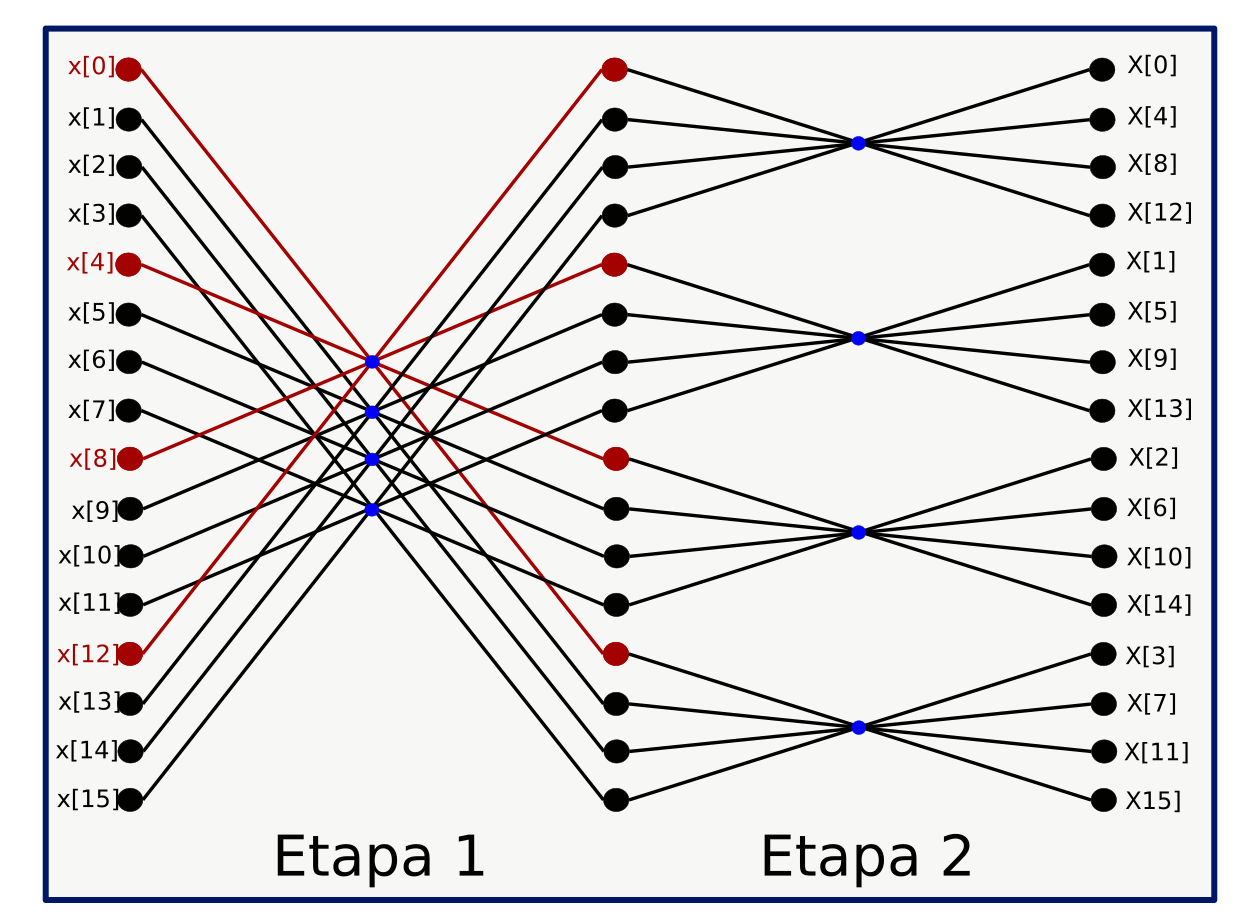
\includegraphics[width=10cm]{./figures/r4_16.png}
        \caption{Esquema de una FFT radix-4 de 16 puntos}
        \label{fig:r4_diag}
\end{figure}

Este funcionamiento implica que para realizar un cálculo aritmético se deben tener almacenados en
memoria tres puntos, que deben ser extraídos de memoria al entrar el cuarto punto para realizar el
cálculo. Luego del cálculo se obtienen cuatro puntos de los cuales tres son almacenados en memoria
mientras que el cuarto punto es utilizado en la etapa siguiente.


En la figura \ref{fig:radix4blocks} se muestra un diagrama en bloques simplificado de la
arquitectura radix-4 iterativa. Se diferencian claramente tres partes, la memoria, de tres entradas
y tres salidas, la unidad aritmética conformada por el \textit{dragonfly} (nombre que se le asigna
al sumador/restados cuádruple que realiza las operaciones en la radix-4), el multiplicador, y la
unidad de control. 
Esta arquitectura presenta un nivel superior de complejidad que la radix-2 que se traduce
principalmente en una unidad de control más compleja y la unidad aritmética que puede ser un poco
más lenta reduciendo así la frecuencia máxima de trabajo. Pero a su vez ofrece la ventaja de
requerir la mitad de etapas que la radix-2 para realizar el cómputo de una FFT de la misma cantidad 
de puntos.

\begin{figure}[htb!]
        \centering
        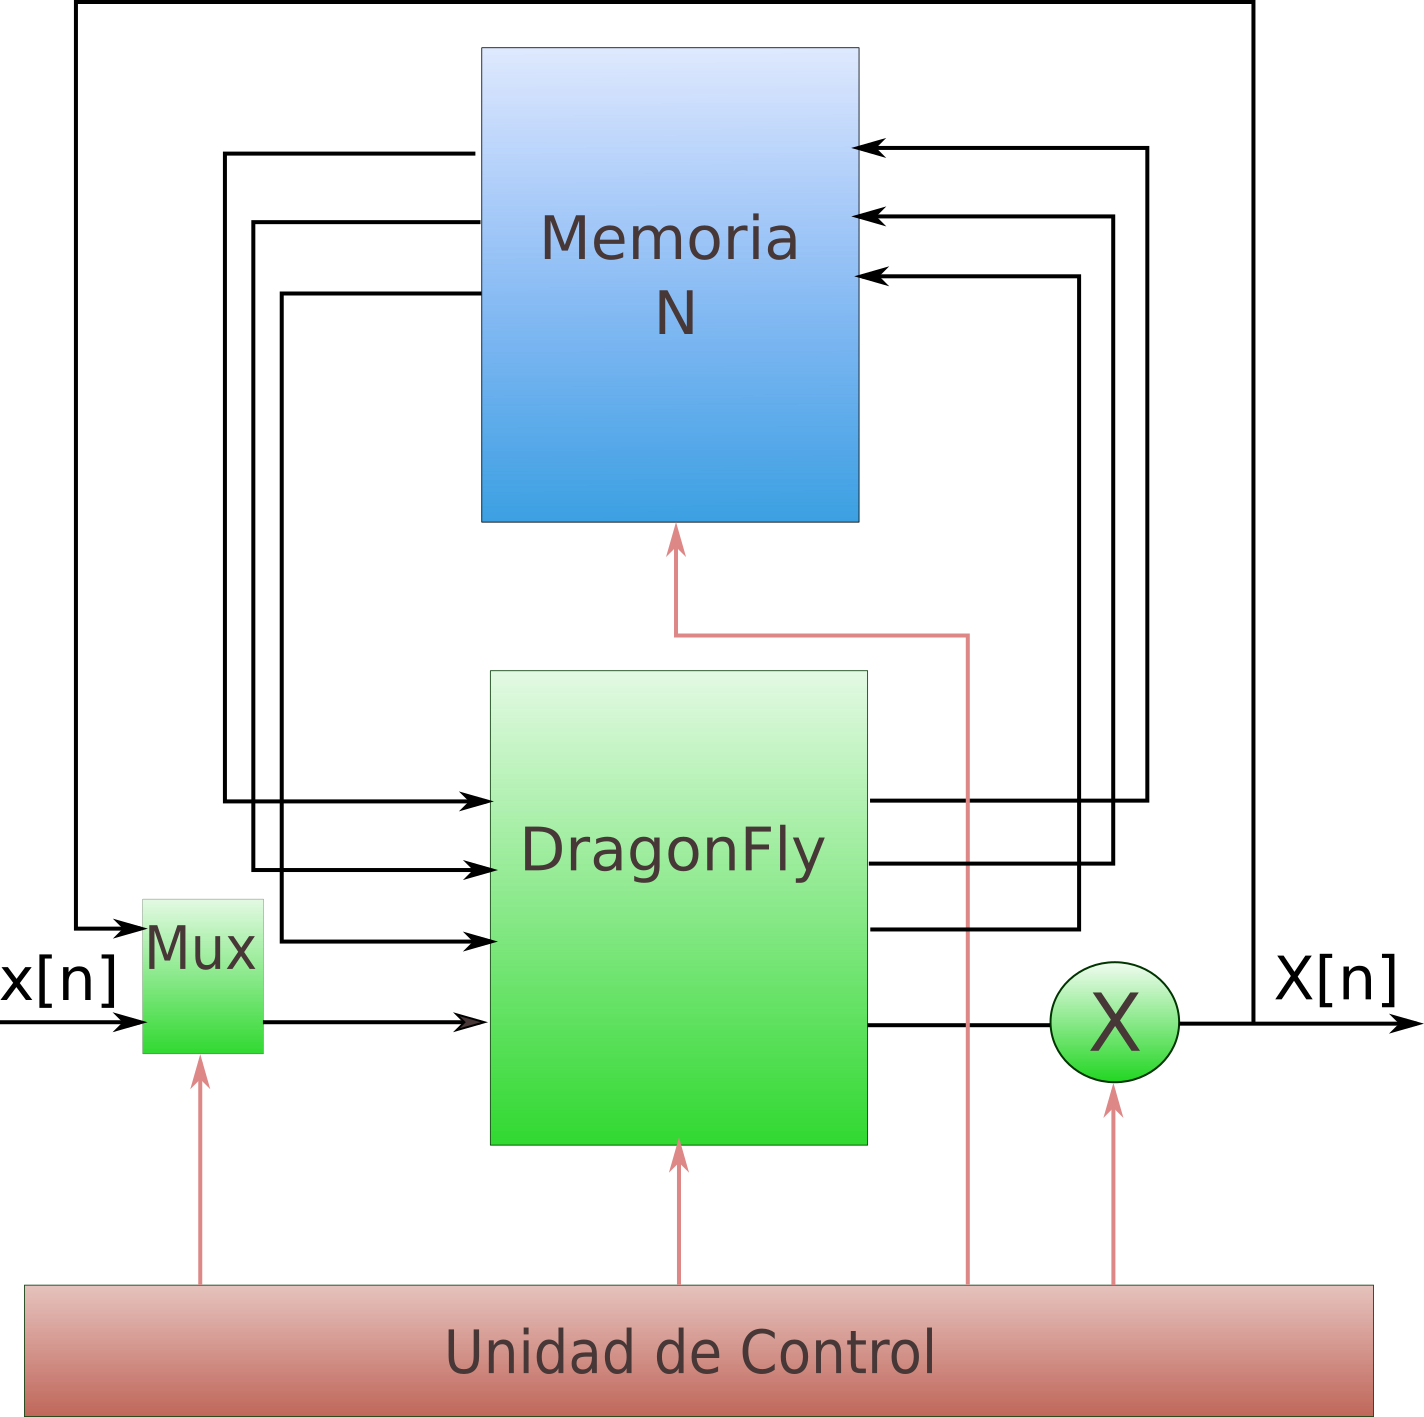
\includegraphics[width=10cm]{./figures/radix4blocks.png}
        \caption{Diagrama simplificado de la arquitectura radix-4 iterativa}
        \label{fig:radix4blocks}
\end{figure}

\subsection{Memoria} \label{sec:r4mem}

Como se explicó, en la arquitectura radix-4 se deben escribir y leer de memoria tres puntos en forma
simultánea cada vez que se realiza una operación aritmética.
En la figura \ref{fig:tripleRam} se presenta el bloque de memoria RAM de triple entrada y triple
salida con sus puertos de conexión. Los valores entre corchetes indican el tamaño del bus
correspondiente.

\begin{figure}[htb!]
        \centering
        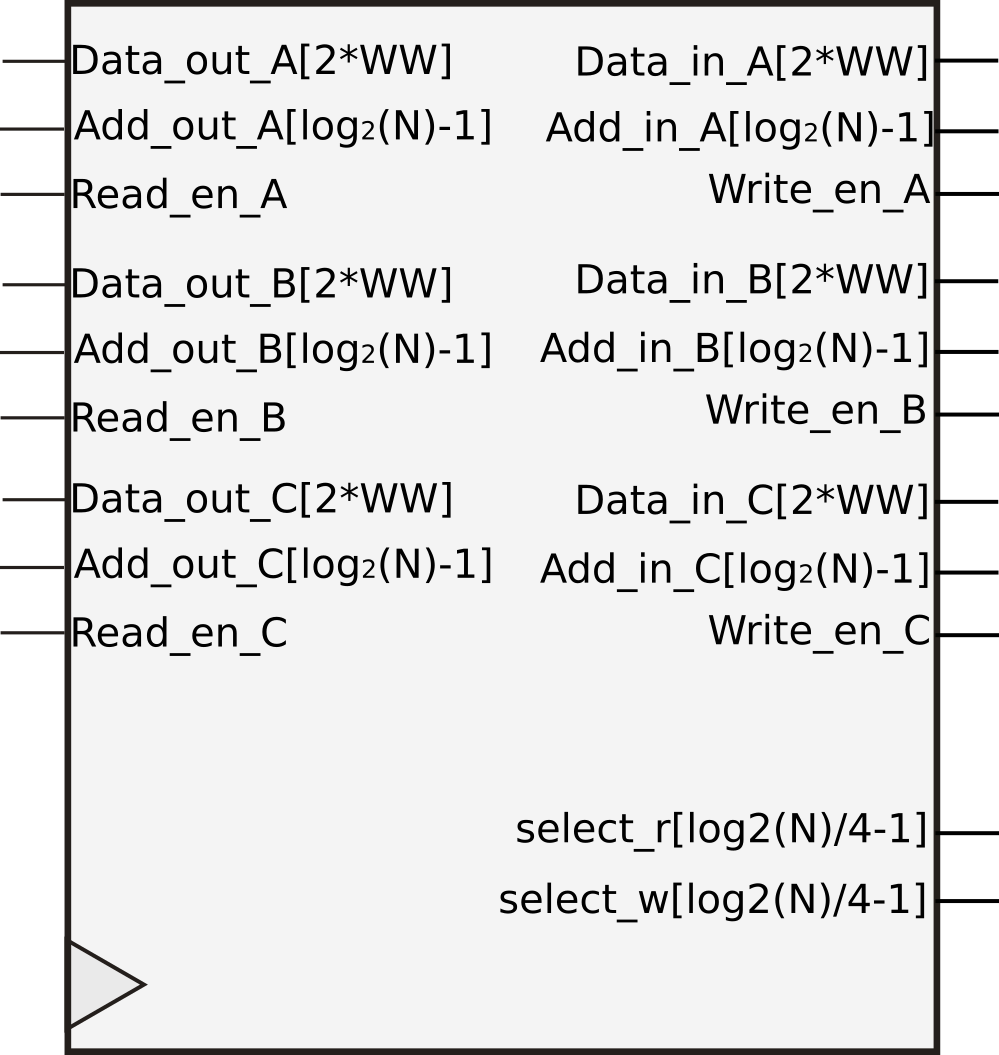
\includegraphics[width=6cm]{./figures/tripleRAM.png}
        \caption{RAM de triple entrada y triple salida}
        \label{fig:tripleRam}
\end{figure}

El bloque tiene tres puertos de entrada y tres puertos de
salida, cada uno con sus correspondientes señales de datos, dirección y habilitación. Las señales
select\_r y select\_w se utilizan para determinar, en conjunto con la señal de dirección de cada
puerto, en que región de la memoria esribir.\\

Como es necesario poder leer y escribir en tres posiciones de memoria simultáneas se construye el
bloque de memoria RAM de triple entrada y triple salida utilizando tres subbloques RAM de doble
puerto igual a los utilizados en la radix-2 (subsección \ref{sec:r2mem}). Se hace de esta manera ya que al
sintetizar en una FPGA, los bloques de memoria RAM de doble puerto se sintetizan utilizando los
bloques RAM propios de la FPGA optimizando la utilización de recursos.


Cada uno de los tres subbloques RAM que componen el bloque triple tiene una capacidad de
almacenamiento de $N/3$ puntos. La distribución de los puntos en los tres subbloques se realiaza de
forma que en cada operación aritmética de cuatro puntos, haya un punto entrando a la unidad
aritmética desde la entrada a la arquitectura o desde la etapa anterior y los restantes tres
provenientes de cada uno de los subbloques RAM, para obtenerlos en forma simultánea. Del mismo
modo, de los cuatro resultados de la operación aritmética, uno se reserva para la etapa siguiente y
los tres restantes se almacenan cada uno en sendos subbloques RAM simultáneamente.

Como el acceso a las posiciones de memoria no es siempre a direcciones continuas, ya que al ser una
arquitectura iterativa se ejecuta sucesivamente una operación de cada etapa, se direccionan los
subbloques de memoria de manera que queden delimitadas las porciones de memoria correspondientes a
cada etapa, como se muestra en la figura \ref{fig:tripleRamdir}. Cada una de estas regiones es de
tamaño igual a $\frac{1}{4}$ de la longitud de la FFT de la etapa correspondiente, por ejemplo la porción de memoria correspondiente a la primer etapa
será $\frac{N}{4}$ en cada subbloque, comprendiendo en total $\frac{3N}{4}$, para la segunda
etapa cada subbloque reservará $\frac{\log_4(N)}{4}$ ya que cada FFT de la segunda etapa es de
longitud $\log_4(N)$, así hasta llegar a la última etapa donde solo se reserva una posición de
memoria de cada subbloque, almacenando en el bloque completo los tres puntos necesarios para
realizar un cálculo aritmético cuando llegue el siguiente punto de la etapa
anterior.

Para direccionar la memoria se utiliza un vector de dirección de $\log_2(N)-1$, que si bien
permitiría direccionar $N/2$ posiciones de memoria aquí se lo utiliza para direccionar $N/3$ ya que
un vector de direcciones de $\log_2(N)-2$ solo permite direccionar $N/4$ posiciones.
Para obtener la dirección de la posición que se debe leer o escribir se utiliza como base el
contenido de la entrada de dirección del subbloque correpondiente y se le aplica un enmascarado con
el valor de la entrada de selección (select\_r o select\_w) que asignan valores a los bits de mayor
valor de la palabra de dirección, permitiendo así leer o escribir en la posición respectiva a la
dirección base en la región que corresponda a la etapa actual del cómputo de la FFT.

\begin{figure}[htb!]
        \centering
        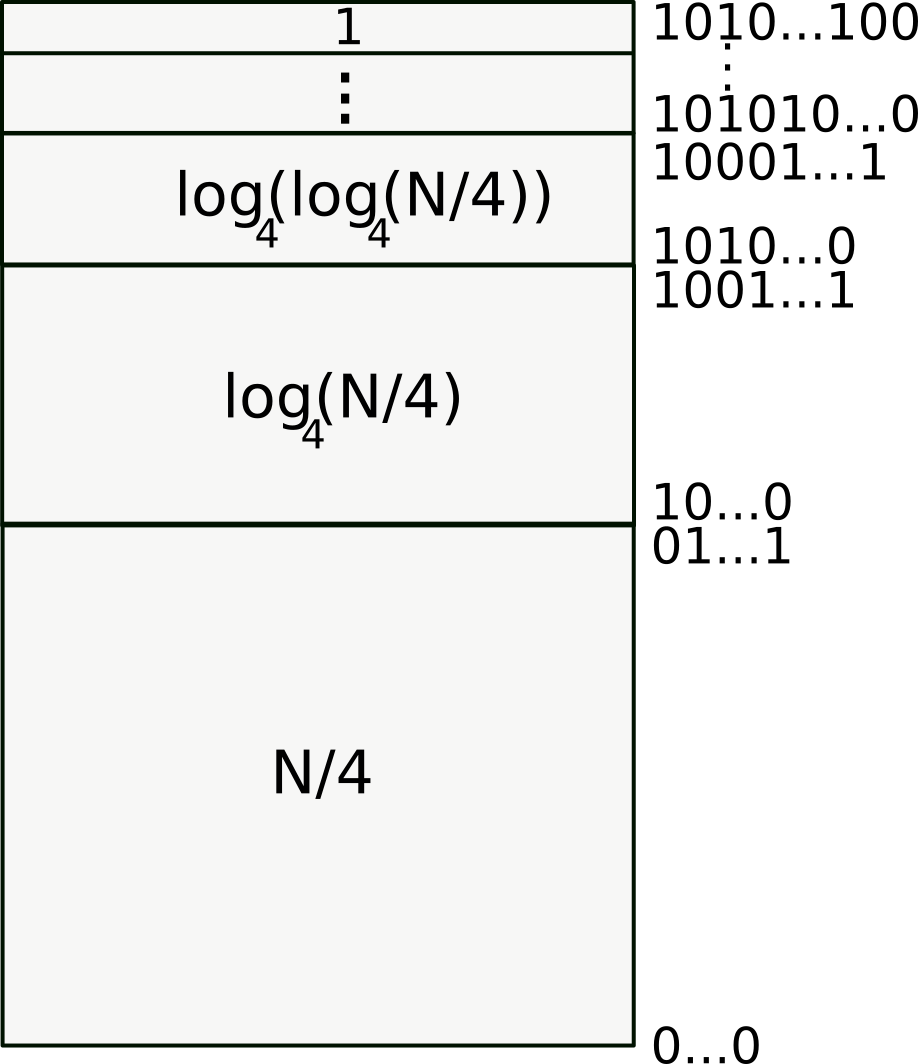
\includegraphics[width=6cm]{./figures/tripleRAMdir.png}
        \caption{Esquema de direccionamiento de los subbloques RAM}
        \label{fig:tripleRamdir}
\end{figure}

En la figura \ref{fig:tripleRamdir} se muestra esquemáticamente la división de cada subbloque en
regiones a través del direccionado, y las direcciones respectivas al comienzo y final de cada
región. Se ve claramente como quedan direcciones sin utilizar ya que con $\log_2(N)-1$ bits se
podrían direccionar $N/2$ posiciones de memoria, por lo que se utilizan únicamente $2/3$ de las
direcciones posibles.

A través de los controles de habilitación de lectura y escritura se puede acceder individualmente a
cada subbloque RAM de la memoria de triple entrada y triple salida.

\subsection{Sumador/restador}

La unidad aritmética debe resolver las ecuaciones (\ref{eq:radix4_suby}) a (\ref{eq:radix4_subh}).
Para esto se opera directamente transladando dichas ecuaciones a \textit{verilog} teniendo en cuenta
que multiplicar por $j$ es equivalente a intercambiar las partes real e imaginaria (canbiando el
signo de la última) del número complejo. Por la forma que toma cada operación de cuatro puntos en el
diagrama de la figura \ref{fig:r4_diag} se le llama \textit{dragonfly} a la unidad de cómputo
aritmético de la radix-4.

En cada etapa del cómputo de la radix-4 pueden realizarse dos tipos de operaciones, una operación
aritmética entre cuatro puntos o un movimiento de datos en memoria, como sucede en la radix-2. En el
segundo caso, el movimiento a memoria puede ser el almacenamiento de un punto entrante a la arquitectura o
proveniente de una etapa anterior, o la lectura de un punto de memoria para multiplicarlo por un
twiddle factor y almacenarlo nuevamente en la región correspondiente a la etapa siguiente
(corresponde al traspaso de un punto resultante de una operación aritmética de una etapa a la
siguiente pasando por el multiplicador). 
Para las operaciones de movimientos de datos en memoria se
dispone internamente en la unidad aritmética de un sistema de multiplexores que permiten direccionar
la entrada del dato de la arquitectura a cualquiera de las tres salidas correspondientes a los tres
subbloques de memoria para su almacenamiento, o direccionar cualquiera de las tres entradas desde
memoria a la salida conectada a la entrada del multiplicador para realizar el traspaso de puntos de
una etapa a la siguiente.

\begin{figure}[htb!]
        \centering
        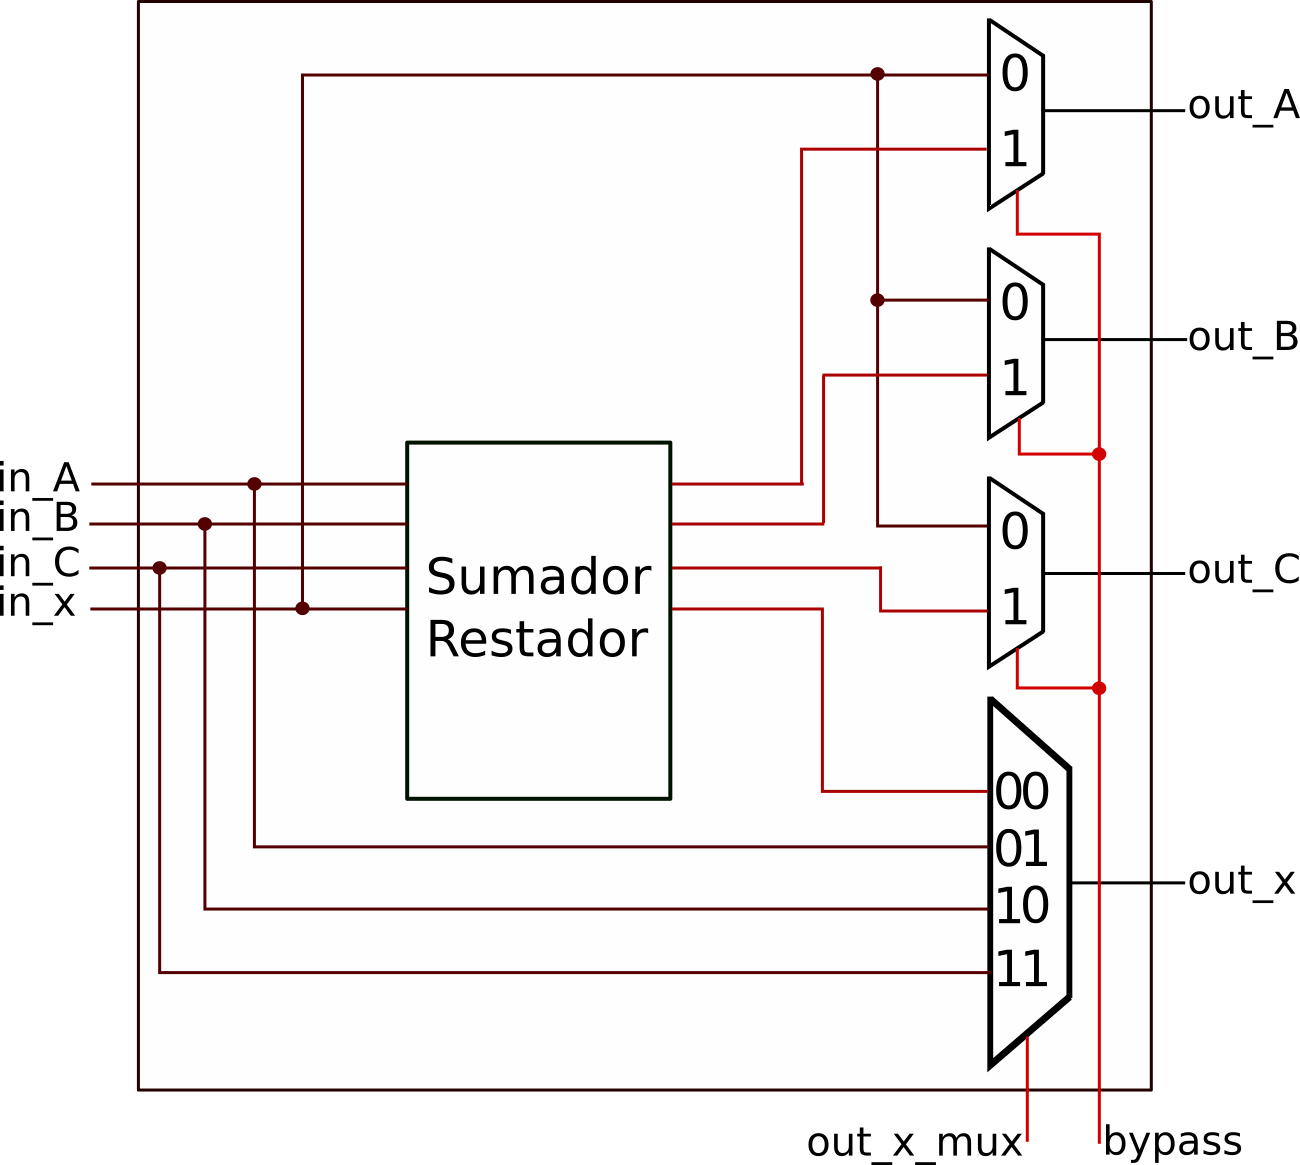
\includegraphics[width=8cm]{./figures/firefly.png}
        \caption{Diagrama de la unidad aritmética incluyendo los multiplexores de bypass}
        \label{fig:firefly}
\end{figure}

En la figura \ref{fig:firefly} se muestra el diagrama en bloque de la unidad aritmética. Se observa
el arreglo de multiplexores que permite direccionar a las salidas a memoria los resultados de la
operación aritmética o la entrada $x$ del bloque. También se observa un multiplexor $4-1$ que
permite seleccionar la salida $x$, conectada al multiplicador, que permite seleccionar entre el
resultado de la operación aritmética o una de las tres entradas de operandos $A, B$ o $C$. 
La unidad aritmética incluye los mecanismos para realizar el redondeo o truncamiento, controlados
por dos señales: una señal de selección de redondeo o truncamiento y una señal de habilitación de 
redondeo/truncamiento individual por etapa. Este mecanismo se detalla en la subsección
\ref{sec:secEscal}.\\
Para almacenar en memoria un dato entrante a la arquitectura se direcciona al subbloque de memoria
correspondiente a través del módulo \textit{dragonfly}, al igual que al extraer un dato de un
subbloque de memoria para enviarlo a la salida de la arquitectura.

\subsection{Datapath}
En la figura \ref{fig:datapathR4} se observa el datapath para la radix-4 iterativa. El bloque
\textit{dragonfly} concentra la unidad aritmética, el algoritmo de redondeo/truncado y el datapath
interno que distribuye las entradas en las diferentes salidas. Los datos entrantes a cada subbloque
de memoria pueden provenir desde la unidad aritmética como resultado de una operación o desde el
\textit{delay register}, proveniente de la etapa anterior.

\begin{figure}[htb!]
        \centering
        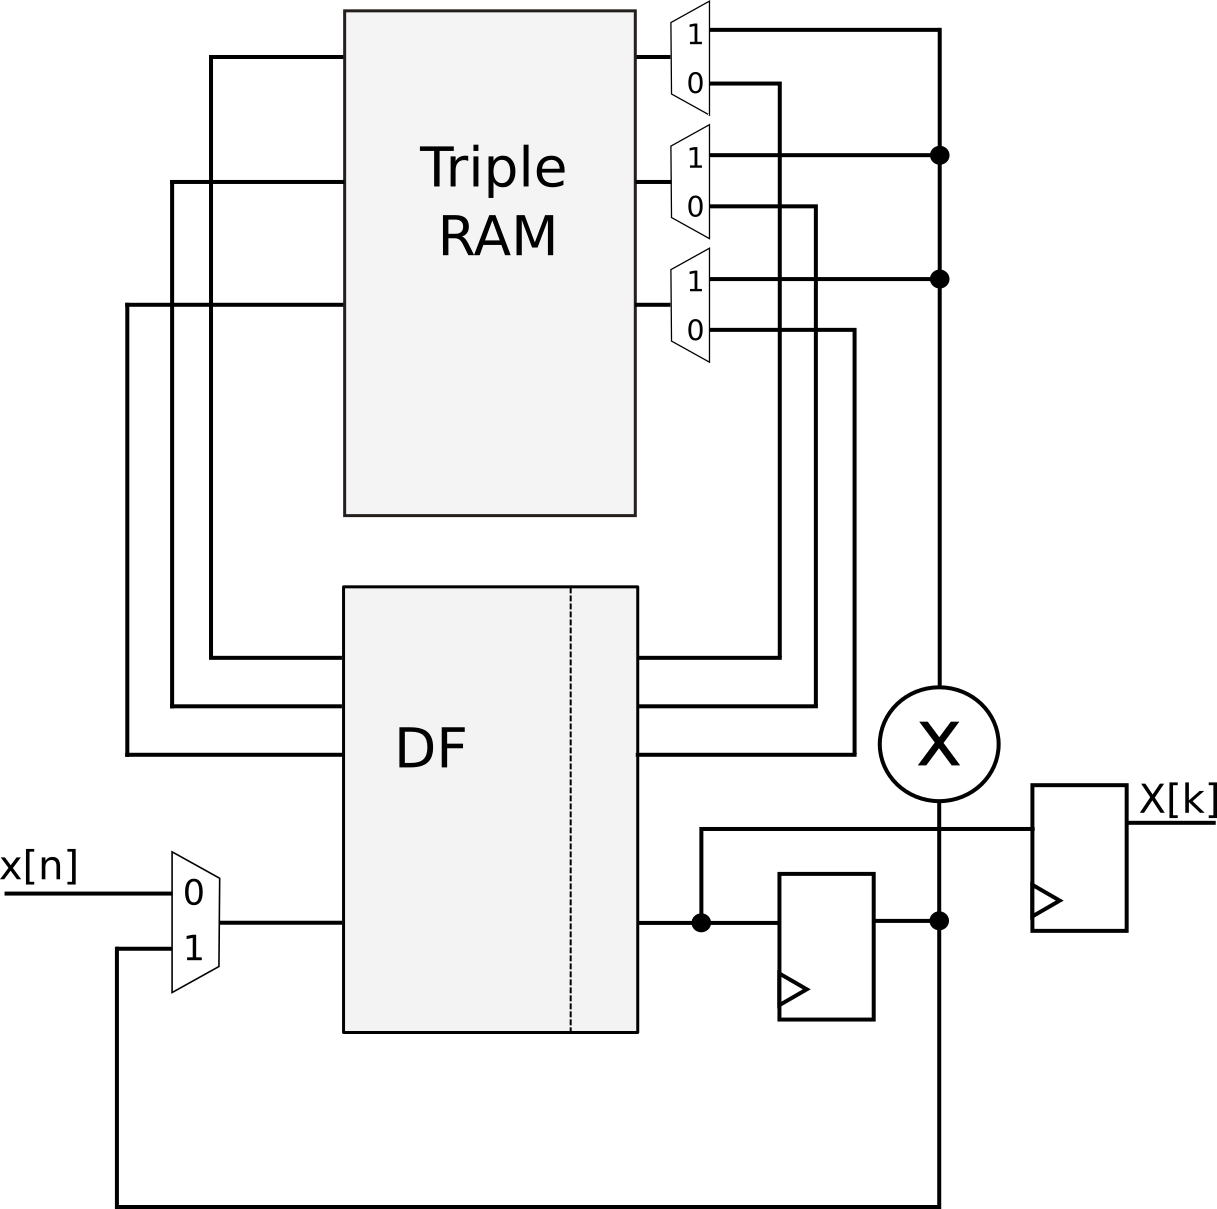
\includegraphics[width=8cm]{./figures/datapathR4.png}
        \caption{Datapath de la arquitectura radix-4 iterativa}
        \label{fig:datapathR4}
\end{figure}

El \textit{datapath} es controlado por la unidad de control a través de los multiplexores de acceso
a memoria, el mumltiplexor de entrada a la unidad aritmética y el \textit{datapath} interno de la
unidad aritmética por medio de sus señales de control.

En la figura \ref{fig:datapathMemR4} se muestran las posibles configuraciones para el
\textit{datapath} para operaciones de transferencia a memoria de acuerdo al tipo de etapa que se
está procesando.
Las líneas punteadas muestran caminos posibles dependiendo del subbloque de memoria donde se desea escribir o leer.

Durante estas operaciones, dependiendo de si la entrada es inicial, intermedia o final, se toma el
dato de entrada de la arquitectura o de la etapa anterior y se envía a memoria, y se lee un dato de
memoria y se envía al \textit{delay register} para ser luego multiplicado por el twiddle factor y
ser guardado en memoria en la etapa siguiente, o enviado a la salida de la arquitectura en caso
de estar ejecutándose la etapa final.\\

\begin{figure}[htb!]
        \centering
        \begin{subfigure}{\columnwidth}\centering
        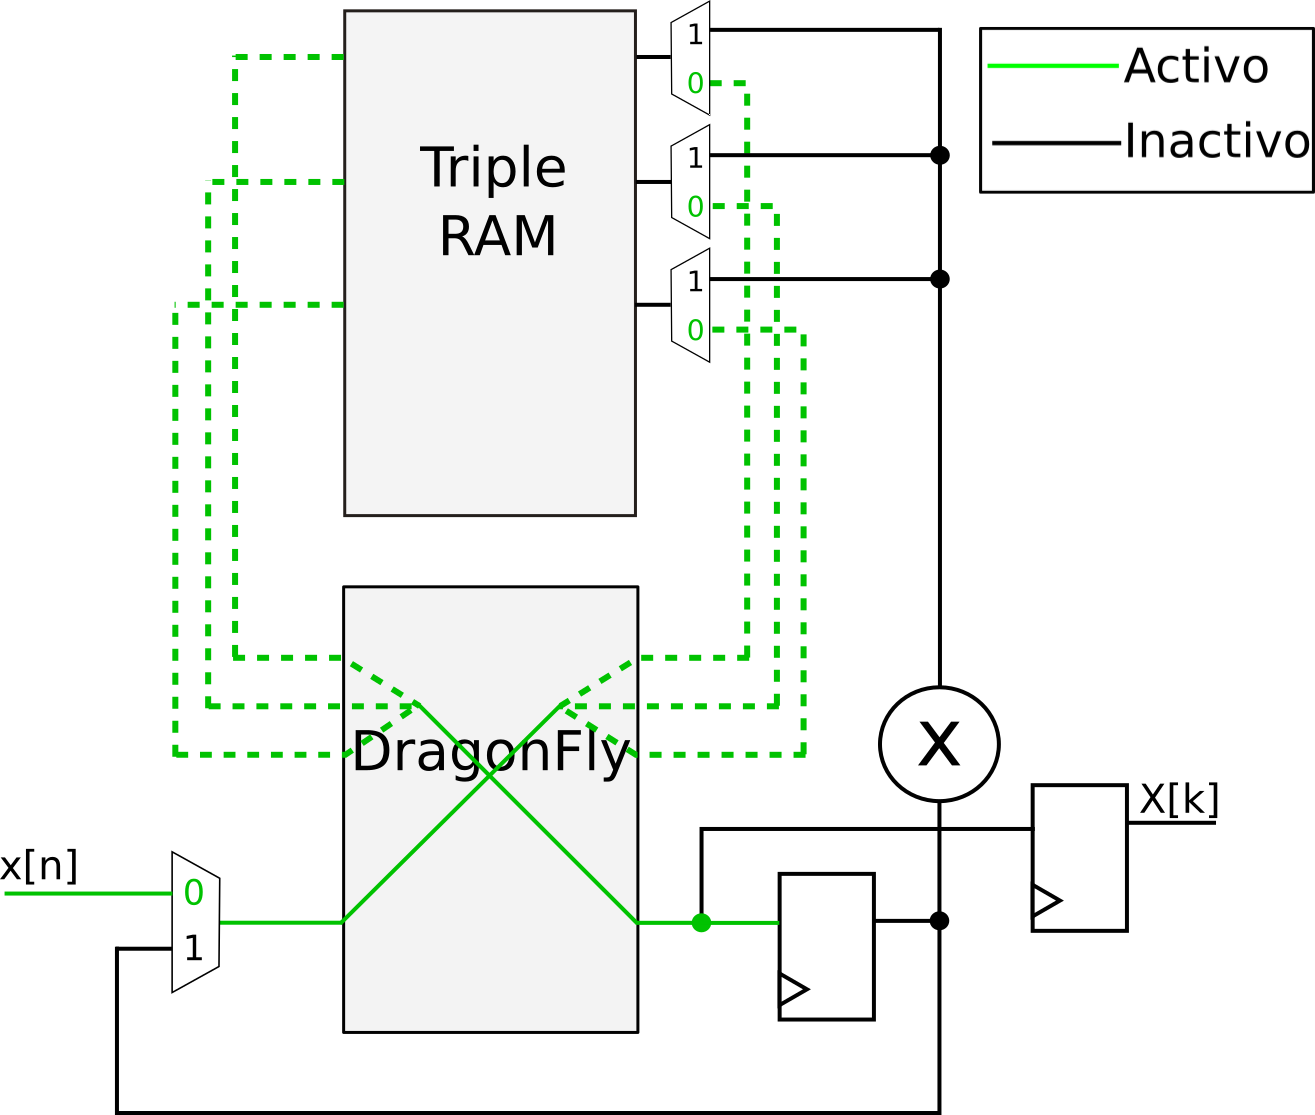
\includegraphics[width=7cm]{./figures/datapathR4_mem_ini.png}
        \caption{Etapa inicial}
        \end{subfigure}
        \begin{subfigure}{\columnwidth}\centering
        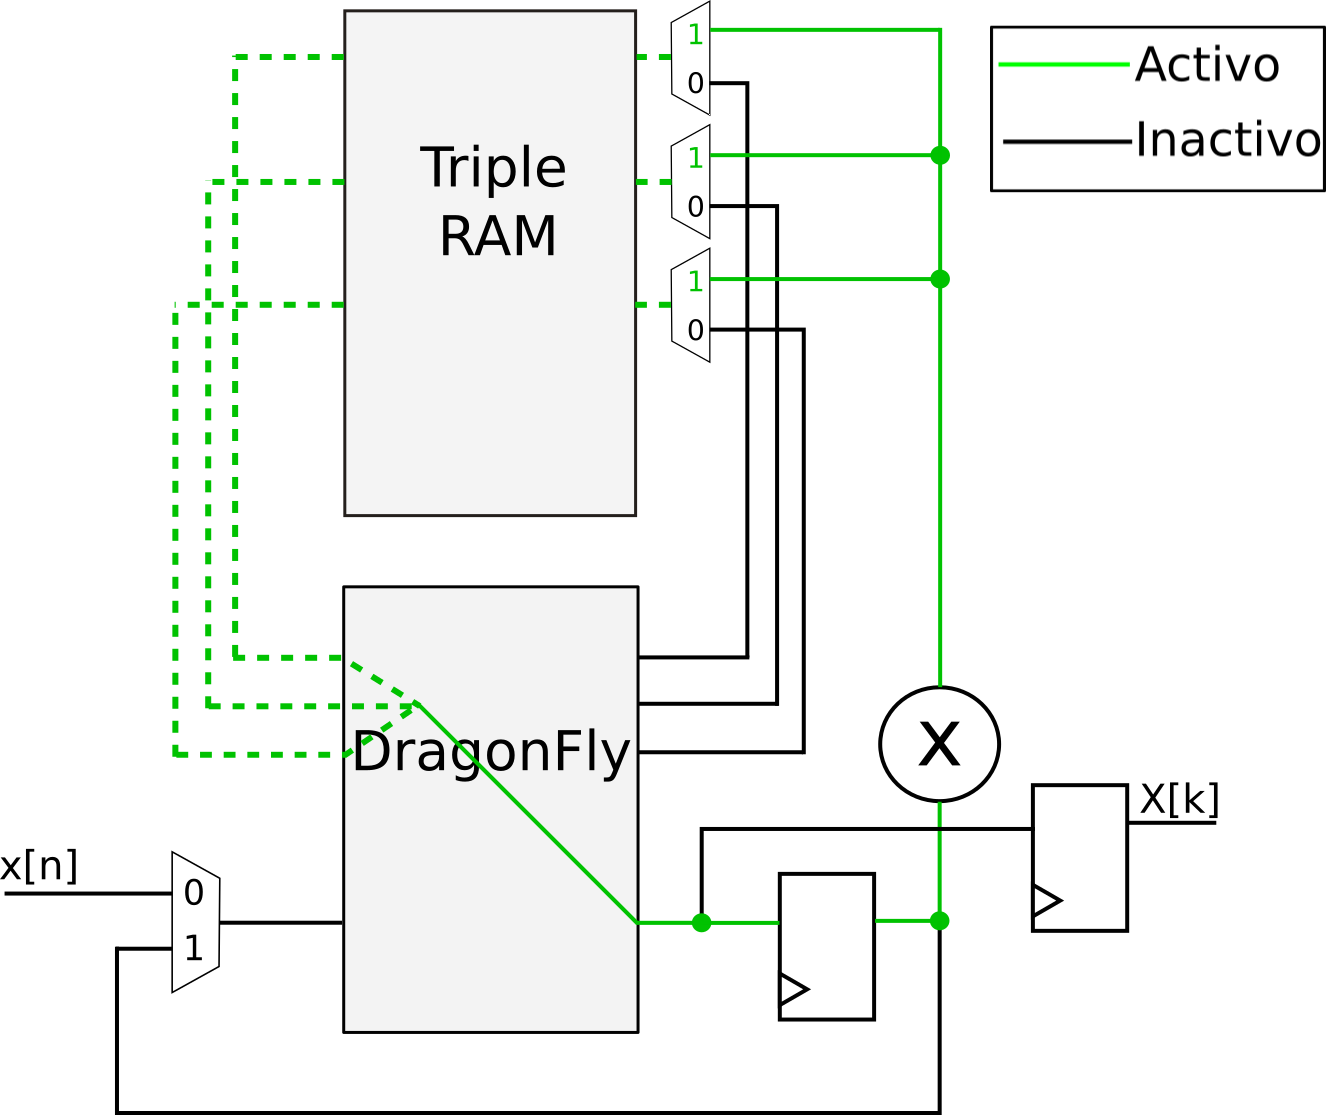
\includegraphics[width=7cm]{./figures/datapathR4_mem_int.png}
        \caption{Etapa intermedia}
        \end{subfigure}
        \begin{subfigure}{\columnwidth}\centering
        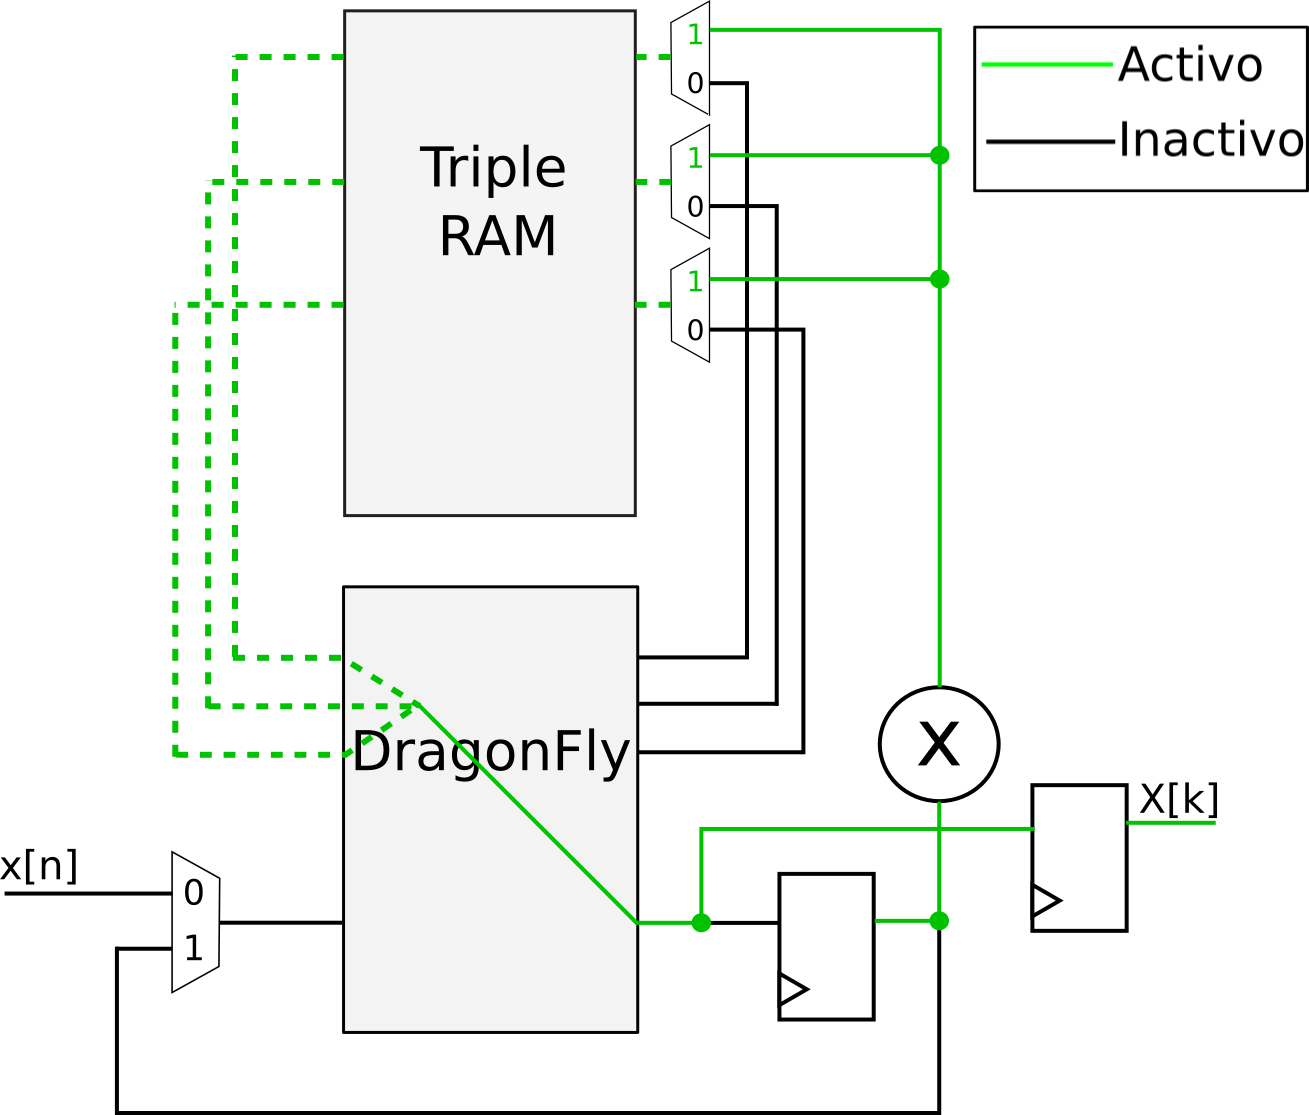
\includegraphics[width=7cm]{./figures/datapathR4_mem_fin.png}
        \caption{Etapa final}
        \end{subfigure}
        \caption{Datapath para operaciones de transferencia en memoria}
        \label{fig:datapathMemR4}
\end{figure}

En la figura \ref{fig:datapathAritR4} se muestran las distintas configuraciones posibles para el
\textit{datapath} para operaciones aritméticas.

Durante estas operaciones se leen tres datos almacenados en memoria y un dato, que dependiendo de si
la etapa que se está procesando es la inicial, una etapa intermedia o la etapa final, proviene de la
entrada de la arquitectura o de la etapa anterior y se los procesa en la unidad aritmética. Una vez
realizada la operación, tres de los resultados son almacenados en memoria y el restante se envía al
\textit{delay register} para su utilización en la etapa siguiente, en caso de estar procesando la
etapa inicial o una etapa intermedia, o a la salida de la arquitectura en caso de ser la etapa
final.

\begin{figure}[htb!]
        \centering
        \begin{subfigure}{\columnwidth}\centering
        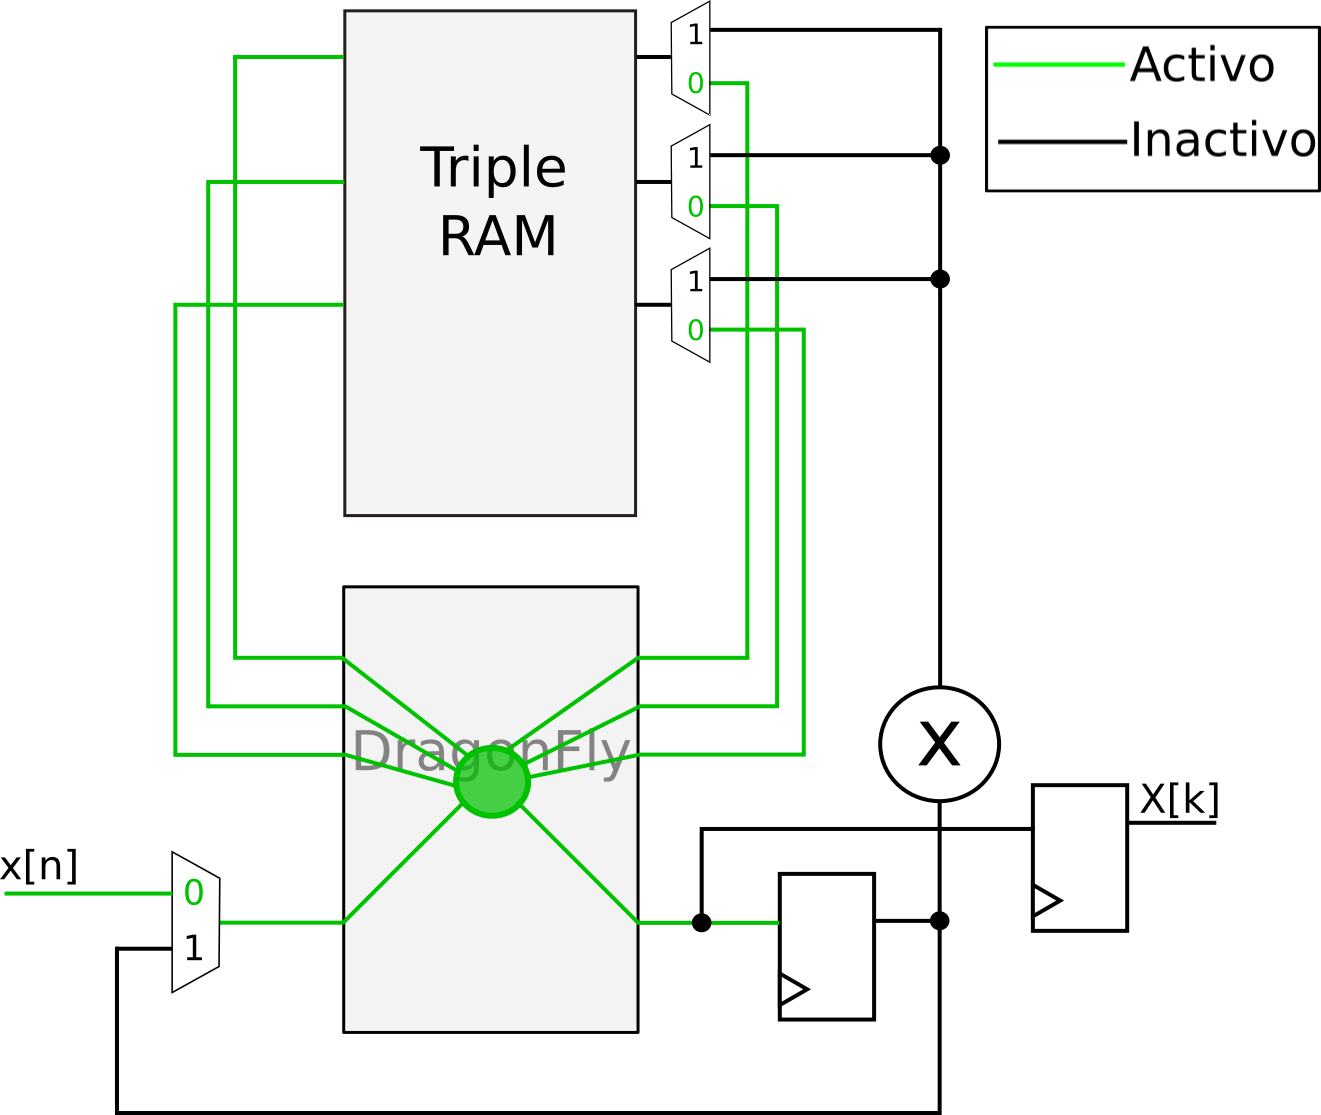
\includegraphics[width=7cm]{./figures/datapathR4_arit_ini.png}
        \caption{Etapa inicial}
        \end{subfigure}
        \begin{subfigure}{\columnwidth}\centering
        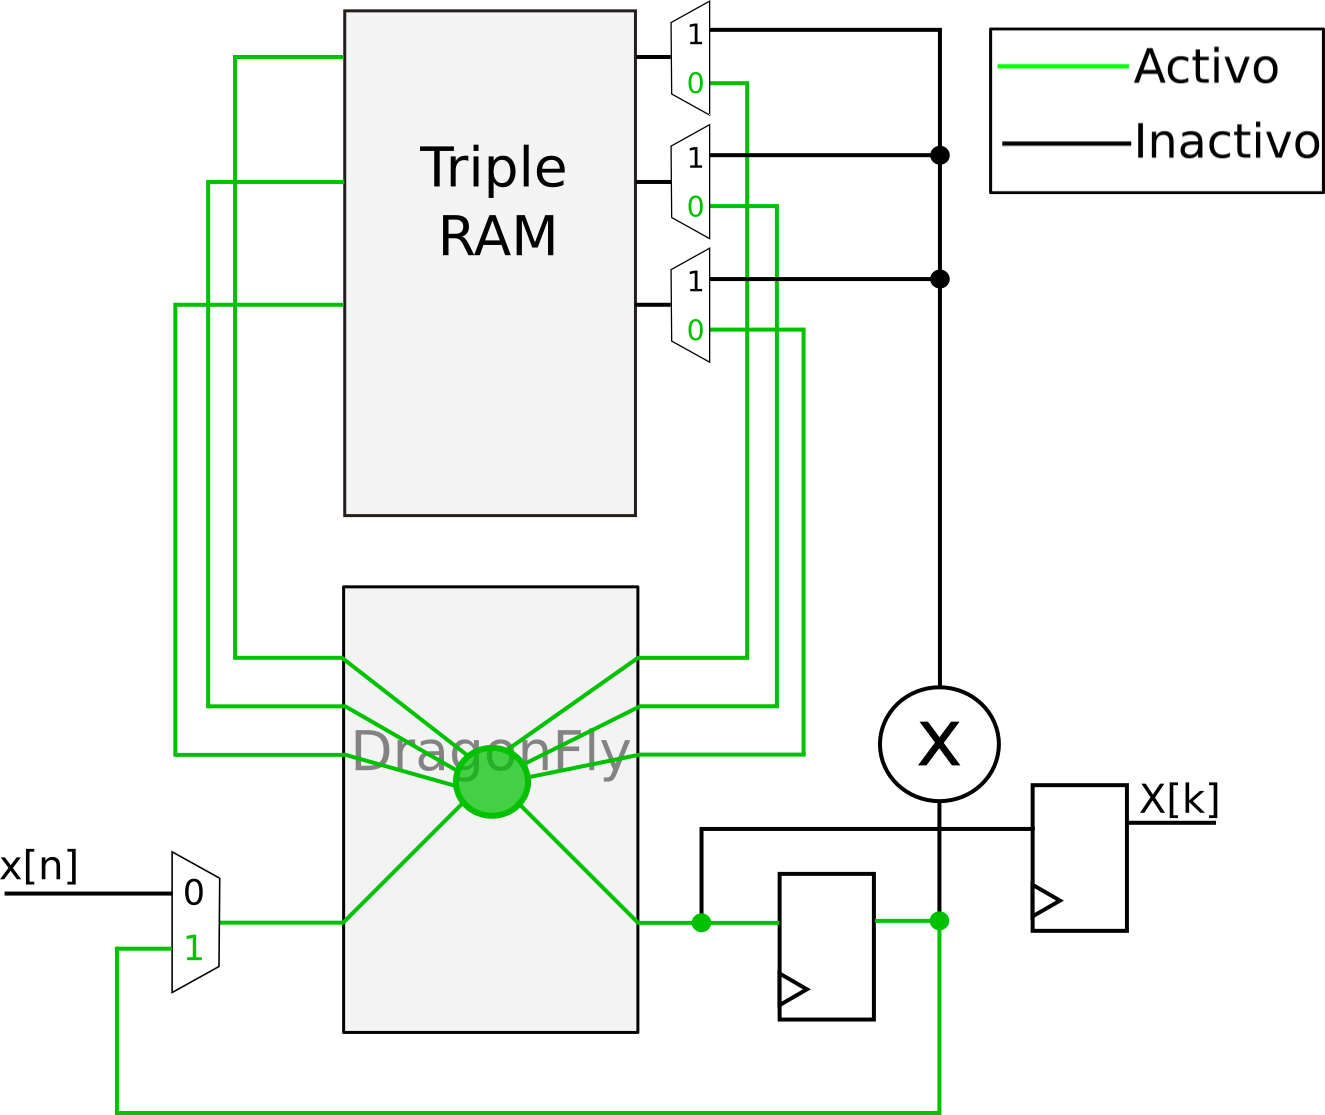
\includegraphics[width=7cm]{./figures/datapathR4_arit_int.png}
        \caption{Etapa intermedia}
        \end{subfigure}
        \begin{subfigure}{\columnwidth}\centering
        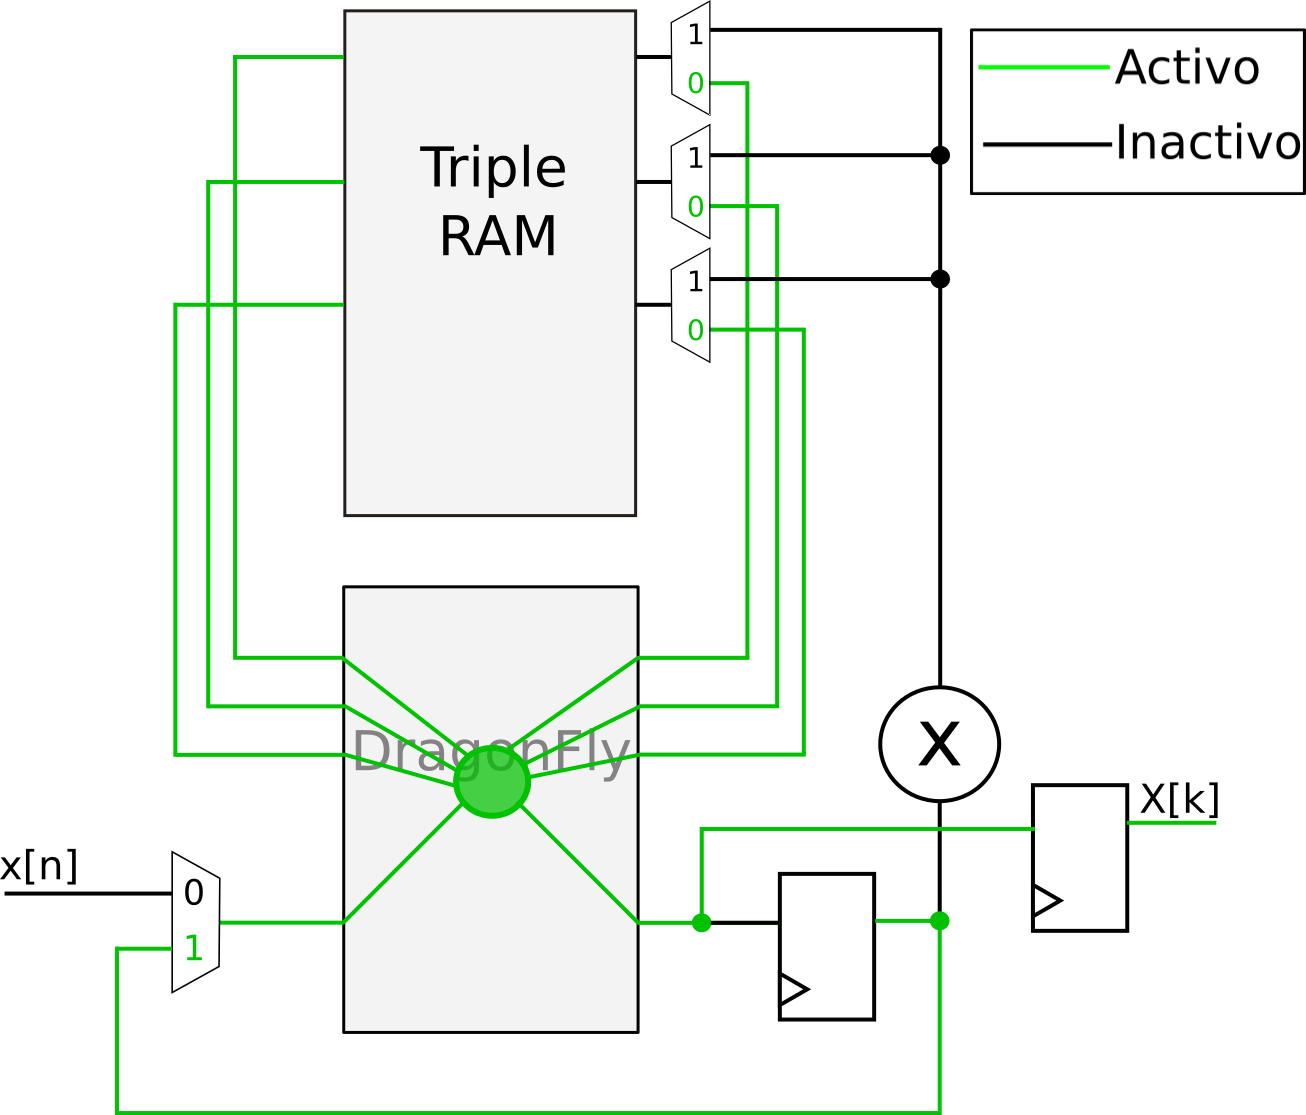
\includegraphics[width=7cm]{./figures/datapathR4_arit_fin.png}
        \caption{Etapa final}
        \end{subfigure}
        \caption{Datapath para operaciones en butterfly}
        \label{fig:datapathAritR4}
\end{figure}

En la arquitectura radix-4 iterativa propuesta se pueden identificar tres tipos distintos de etapas,
la etapa inicial, las intermedias y la final, en las que pueden ejecutarse una de dos posibles
operaciones: una transferencia de un dato a memoria o una operación aritmética. El tipo de etapa
que se está procesando y el tipo de operación que se realiza en esa etapa determinan la
configuración del datapath en cada ciclo de \textit{clock}.\\

A continuación se listan las posibles configuraciones de \textit{datapath} para cada tipo de etapa y
operación:

\begin{itemize}
  \item Etapa inicial
  \begin{itemize}
    \item Operaciones aritméticas: tres datos almacenados en memoria y el dato
    de entrada a la arquitectura. Tres de los resultados son almacenados en memoria mientras que el
    cuarto se envía al multiplicador.
    \item Transferencia a memoria: se almacena el dato entrante a la arquitectura en uno de los tres
    subbloques de memoria.
  \end{itemize}
  \item Etapas intermedias
  \begin{itemize}
    \item Operaciones aritméticas: tres datos almacenados en memoria y el dato de la etapa anterior
    alacenado en el \textit{delay register}. Tres de los resultados son almacenados en memoria mientras que el
    cuarto se envía al multiplicador.
    \item Transferencia a memoria: se extrae un dato de memoria y se envía al multiplicador mientras
    se almacena en memoria el dato de la etapa anterior almacenado en el \textit{delay register}.
  \end{itemize}
  \item Etapa final
  \begin{itemize}
    \item Operaciones aritméticas: tres datos almacenados en memoria y el dato de la etapa anterior
    alacenado en el \textit{delay register}. Tres de los resultados son almacenados en memoria mientras que el
    cuarto se envía a la salida de la arquitectura.
    \item Transferencia a memoria: se extrae un dato de memoria y se envía a la salida de la
    arquitectura mientras se almacena en memoria el dato de la etapa anterior almacenado en el
    \textit{delay register}.
  \end{itemize}
\end{itemize}

\subsection{Unidad de control}

La unidad de control debe contener la lógica necesaria para controlar el funcionamiento de la
arquitectura. Está compuesta por una máquina de estados principal que controla el funcionamiento
general de la arquitectura, y una máquina de estados secundaria que configura el \textit{datapath}
de acuerdo al tipo de etapa y operación que se debe procesar.\\
La unidad de control además de configurar el \textit{datapath} debe controlar el direccionamiento de
la memoria, así como sus señales de control, y generar los \textit{twiddle factors} para el
multiplicador.\\

Al tratarse de una arquitectura radix-4, entra a la arquitectura un punto cada $\log_4(N)$ ciclos de
\textit{clock}, y este es también el número de etapas de la arquitectura, se tiene  un contador de
longitud $\log_2(\log_4(N))$ puntos para identificar el estado que se está procesando en cada ciclo
de \textit{clock}. El desborde de este contador alimenta un contador de longitud $\log_2(N)$ que
cuenta la cantidad de puntos que han ingresado a la arquitectura y permite controlar en que estado
del cómputo total se encuentra. Con estos dos contadores se lleva el control de la máquina de
estados que controla el \textit{datapath} y la memoria, y la generación de los \textit{twiddle
factors}.

Como se ve en la figura \ref{fig:r4_diag}, para una radix-4 de $16$ puntos, en la primer etapa hay
que almacenar en memoria los primeros $12$ puntos hasta realizar una operación aritmética con el
decimotercer punto que entra, utilizando también el primer punto, el quinto y el noveno. En la
segunda etapa se deben almcenar los primeros tres puntos que llegan y recién realizar la operación 
aritmética con el cuarto punto. Cada almacenamiento en memoria puede hacerse a uno de los tres
subbloques, por lo que debe diferenciarse a que subbloque pertenece cada punto que ingresa a una
etapa.

Para decidir si se debe realizar una operación aritmética o una transferencia a memoria, y en este
caso en que se subbloque se debe almacenar el dato, se utilizan dos bits del contador de puntos de
la siguiente manera:

\begin{itemize}
  \item $[00]$ ->  Almacenamiento en subbloque de memoria 1
  \item $[01]$ ->  Almacenamiento en subbloque de memoria 2
  \item $[10]$ ->  Almacenamiento en subbloque de memoria 3
  \item $[11]$ ->  Operación aritmética 
\end{itemize}

Los dos bits del contador de puntos utilizados para determinar la operación a realizar dependen de
la etapa, por lo que se seleccionan de acuerdo al \textit{stg\_ctr} como se muestra en la
\ref{fig:r4conts} para una arquitectura radix-4 de 256 puntos.
 
% Como se explicó en la sección \ref{sec:r4mem}, los subbloques deben almacenar los puntos de manera
% que en cada operación aritmética se encuentre cada uno de los tres datos a extraer de memoria en
% subloques diferentes. Por esto, para la primer etapa del diagrama de la figura \ref{fig:r4_diag} se
% deben almacenar en cada subbloque cuatro puntos en forma consecutiva y luego pasar al subbloque
% siguiente. Para lograr esta diferenciación se leen los bits del contador de puntos de a pares
% utilizando el contador de etapas como índice, comenzando del bit más alto del contador de puntos,
% como se indica en la figura \ref{fig:r4conts}, ejemplificando con dos pares de bits para valores del
% contador de estados (\textit{st\_ctr}) de $0$ y $2$.

\begin{figure}[htb!]
        \centering
        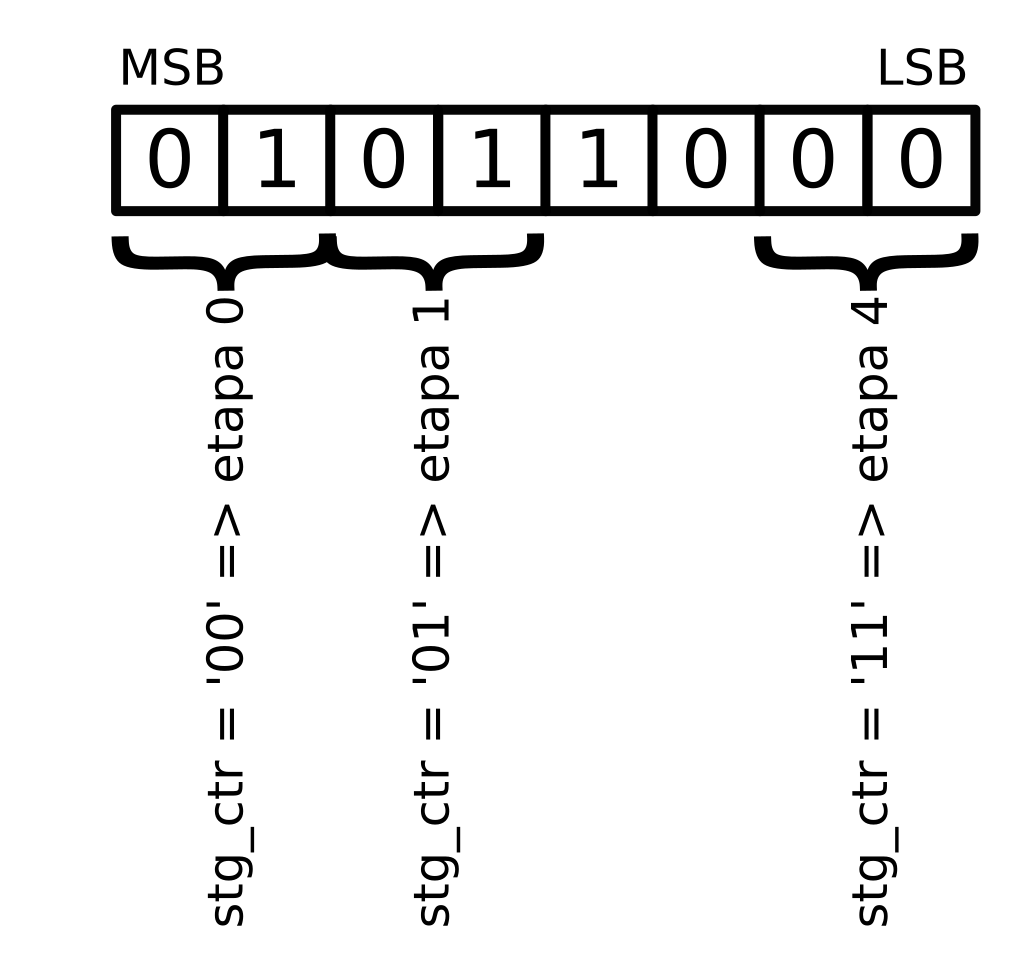
\includegraphics[width=6cm]{./figures/r4conts.png}
        \caption{Selección del par de bits del contador de puntos a evaluar}
        \label{fig:r4conts}
\end{figure}

\subsubsection{Máquinas de estados}

En la figura \ref{fig:r4statep} se muestra el diagrama de estados y transiciones la máquina de
estados principal.
El estado
\textit{Idle} es el estado inicial de la arquitectura. La señal start pasa la máquina al estado \textit{Init}
donde inicializa los parámetros de la arquitectura necesarios para comenzar a procesar y lee el
primer dato de entrada a la arquitectura. Un ciclo de \textit{clock} después la máquina pasa
automáticamente al estado \textit{enabled}.

\begin{figure}[htb!]
        \centering
        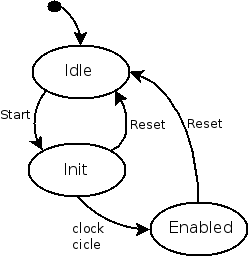
\includegraphics[width=7cm]{./figures/SMr2gen.png}
        \caption{Diagrama de estados y transiciones de la máquina de estados principal}
        \label{fig:r4statep}
\end{figure}

En el estado \textit{Enabled} se identifica la etapa que se está procesando y se configura el
\textit{datapath} para realizar la operación correspondiente. Para esto se utiliza la máquina de
estados secundaria, cuyo estado depende del valor de los bits del contador de puntos
correspondientes a la etapa actual.

\begin{figure}[htb!]
        \centering
        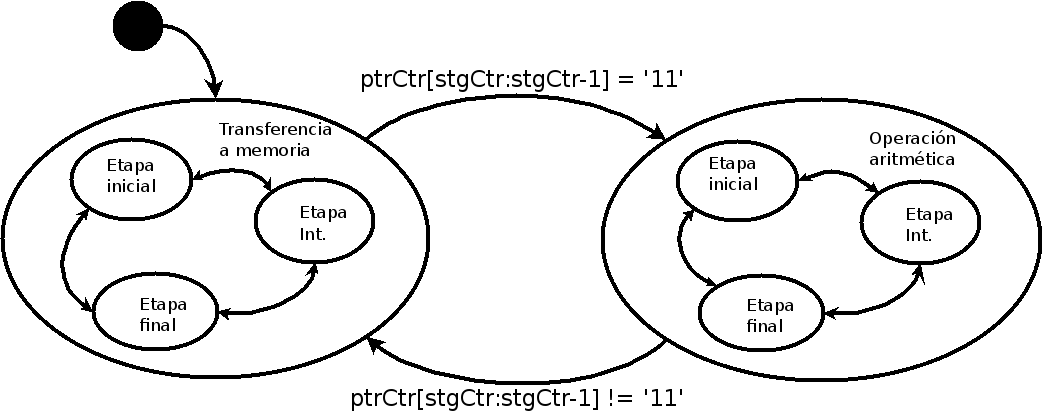
\includegraphics[width=13cm]{./figures/SMr4op.png}
        \caption{Diagrama de estados y transiciones de la máquina de estados secundaria}
        \label{fig:r4stateop}
\end{figure}

En la figura \ref{fig:r4stateop} se observa la máquina de estados secundaria. Dentro de cada uno de
los estados principales se evalúa el tipo de etapa para la configuración del \textit{datapath}.
En cada uno de los estados principales funciona una submáquina de estados que realiza ajustes
menores de acuerdo a si la etapa actual es la etapa inicial, una intermedia o la etapa final. $ptrCtr[stgCtr:stgCtr-1]$ hace
referencia a los dos bits del contador de puntos correspondientes al valor del contador de etapas.\\
Esta máquina de estados controla además la señal de habilitación de escalamiento para la etapa
actual de acuerdo al vector de escalamiento de entrada a la arquitectura. También controla, a través
del contador de puntos y el de etapas, las señales de \textit{handshaking} de salida, indicando si
el dato de salida es un dato válido, señal \textit{data\_valid} y si es el punto inicial o final de
la FFT que se está procesanto actualmente, señales \textit{soo} y \textit{done} respectivamente.

\subsubsection{Control de la memoria}

El control de la memoria se realiza mediante los direccionamientos, las señales de habilitación de
lectura y escritura, y las señales de selección de la región de memoria de cada subbloque donde se
realizará la operación.

El direccionamiento de escritura se realiza directamente mapeando el valor del contador de puntos a
la dirección de escritura. El direccionamiento de lectura se realiza mapeando a la dirección de
lectura el valor del contador de puntos correspondiente al ciclo siguiente de \textit{clock} ya que
en cada flanco positivo del \textit{clock} la memoria dispone a la salida el dato guardado en la
dirección presente en el puerto de dirección de lectura durante el flanco.

Las señales de habilitación de lectura y escritura se controlan dependiendo del valor de los bits
correspondientes del contador de puntos, habilitando el subbloque de memoria correspondiente para
los casos de movimientos en memoria y habilitando los tres subbloques simultáneamente para el caso
de operaciones aritméticas.

Las señales de selección de la región de memoria se controlan utilizando el contador de etapas, ya
que cada región de memoria en un subbloque particular se utiliza para una etapa determinada. Las
señales de selección se construyen como una máscara para lo bits superiores de la señal de
direccionamiento, para ubicar la dirección indicada por el contador de puntos en la región
correspondiente.

\subsection{Integración de la unidad de control}

En la figura \ref{fig:datapathR4control} se muestra el diagrama del \textit{datapath} de la figura
\ref{fig:datapathR4} con el agregado de las señales de la unidad de control. 

\begin{figure}[htb!]
        \centering
        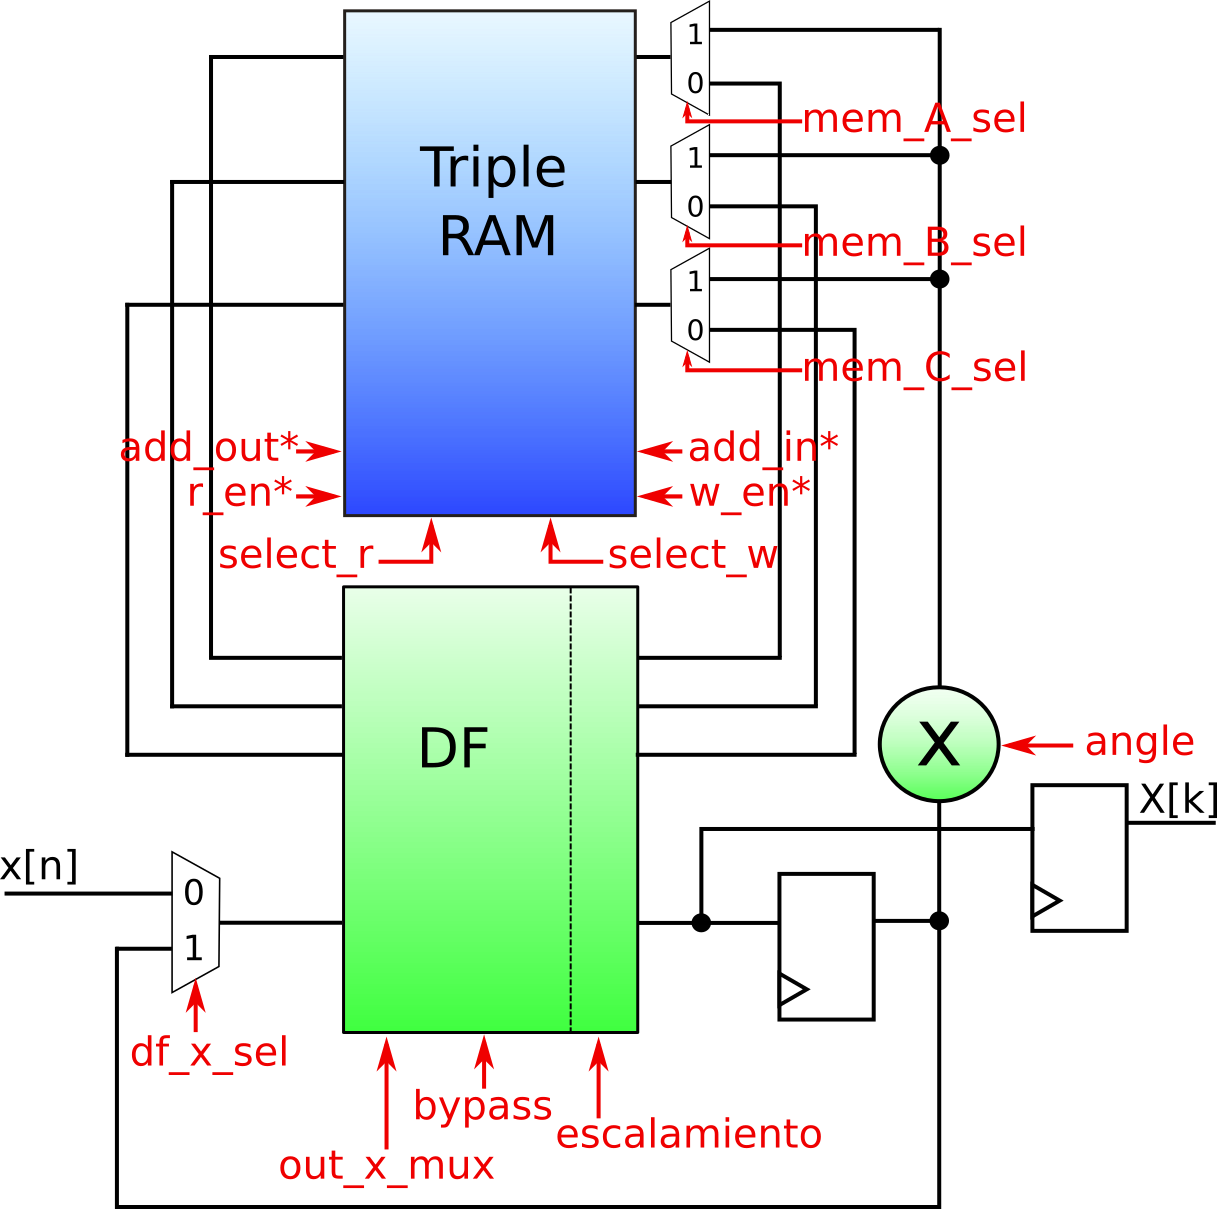
\includegraphics[width=9cm]{./figures/datapathR4control.png}
        \caption{Datapath con las señales de control}
        \label{fig:datapathR4control}
\end{figure}

Las señales de control de la figura \ref{fig:datapathR4control} se listan a continuación, indicando
entre parétesis su tamaño si es mayor a $1$:

\begin{itemize}
  \item \textbf{add\_in*} ($\log_2(N)$) \textit{address in}, dirección de memoria donde se escribirá
  el dato.
  \item \textbf{w\_en*} \textit{write enable}, señal de habilitación de escritura en memoria
  \item \textbf{add\_out*} ($\log_2(N)$) \textit{address out}, dirección de memoria a la que se
  desea acceder.
  \item \textbf{r\_en*} \textit{read enable}, señal de habilitacón de lectura de memoria
  \item \textbf{select\_r} ($\log_2(\log_4(N)))$) Selección de la región de memoria donde se realiza
  la lectura.
  \item \textbf{select\_r} ($\log_2(\log_4(N)))$) Selección de la región de memoria donde se realiza
  la escritura.
  \item \textbf{mem\_A\_sel} señal de control del multiplexor a la entrada al subbloque A de la
  memoria.
  \item \textbf{mem\_B\_sel} señal de control del multiplexor a la entrada al subbloque B de la
  memoria.
  \item \textbf{mem\_C\_sel} señal de control del multiplexor a la entrada al subbloque C de la
  memoria.
  \item \textbf{df\_x\_sel} señal de control del multiplexor de entrada a la unidad aritmética.
  \item \textbf{out\_x\_mux} ($2$) señal de control de la salida $x$ de la unidad aritmética (ver
  esquema en figura \ref{fig:firefly}).
  \item \textbf{out\_x\_mux} señal de control de las salidas a memoria de la unidad aritmética (ver
  esquema en figura \ref{fig:firefly}).
  \item \textbf{angulo} ($N+1$) angulo de rotación para el multiplicador, ya sea cordic o
  multiplicador complejo.
  \item \textbf{escalamiento} señal de indicación de que en la etapa actual se realiza
  redondeo/ truncamiento. 
\end{itemize}

Las señales correspondientes al direccionamiento de memoria, indicadas con un $*$, se muestran
unificadas para simplificar el diagrama, ya que cada subbloque tiene sus propias señales de
control.\\
El bloque indicado como \textit{DF} contiene la unidad aritmética, su \textit{datapath} interno y la
unidad de escalamiento que se describe en la sección \ref{sec:secEscal}.

\section{Módulos compartidos por las dos arquitecturas}
\subsection{Cordic desenrrollado}

Como se explicó en la subsección \ref{sec:twiddlesec}, para el producto por los \textit{twiddle
factors} se implementan dos alternativas distintas. Una de ellas es a través de un módulo de cómputo
del algoritmo cordic, según las ecuaciones desarrolladas en la subsección \ref{sec:cordicsec}.\\

Se utiliza la versión desenrrollada de la arquitectura cordic, ya que permite realizar el cálculo
completo en un solo ciclo de \textit{clock} y si es necesario se puede implementar en forma
\textit{pipelined} colocando registros entre las distintas etapas del cómputo cordic.

La forma de implementar el algoritmo es a través de submódulos consecutivos que realizan las
microrotaciones hasta completar la rotación completa.

En la figura \ref{fig:cordicDiam} se muestra el bloque de cómputo cordic con sus puertos de entradas
y salidas.

\begin{figure}[htb!]
        \centering
        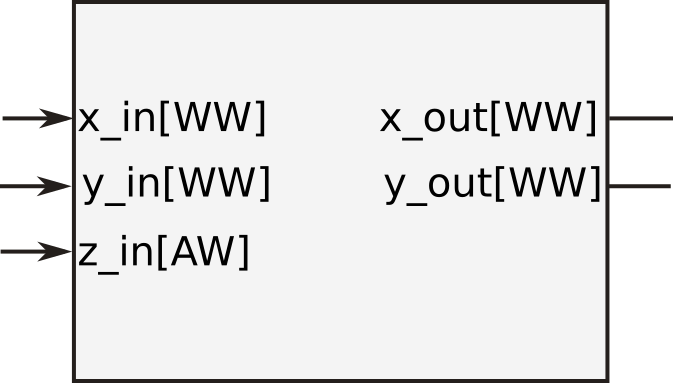
\includegraphics[width=7cm]{./figures/cordicDiam.png}
        \caption{Bloque de módulo de cómputo cordic}
        \label{fig:cordicDiam}
\end{figure}

Los parámetros \textit{WW} y \textit{AW} corresponden a los parámetros globales \textit{Word\_Width},
el ancho de palabra de las entradas de puntos, y \textit{Angle\_Width}, el ancho de palabra del
ángulo de rotación.

Al módulo cordic entra un punto complejo en forma de vector de dos componentes, y el ángulo de
rotación deseado, que representa el \textit{twiddle factor}. Es por esto que las unidades de control
de las dos arquitecturas radix implementadas generan los \textit{twiddle factors} en forma de
ángulos de rotación.
La salida del módulo cordic es el vector de dos dimensiones rotado en el ángulo indicado.\\

Como se indica en la subsección \ref{sec:cordicsec} el algoritmo cordic tiene una cierta ganancia
intrínseca que depende de la cantidad de iteraciones que se realizan. Como se desea que la ganancia
del algoritmo sea $1$ para no modificar la norma del vector de entrada se implementa un módulo de
escalamiento a la salida del módulo cordic para compensar la ganancia de la arquitectura. El valor
por el cual se escala la salida del módulo dependerá de la cantidad de iteraciones que se realicen,
que es un parámetro global de la arquitectura cordic.

Para facilitar la rotación de los vectores de entrada, primero se analiza el ángulo de rotación para
descomponerlo en un primer paso en rotaciones de $90^\circ$ y luego se utiliza el algoritmo cordic para
la rotación final menor al ángulo recto. De este modo, donde el algoritmo se aplica solo a
rotaciones menores a $90^\circ$, se obtienen resultados más precisos con menor cantidad de rotaciones.
También impacta en el tamaño total de la arquitectura, ya que se debe implementar una tabla con los
valores de los $\arctan(\alpha)$ para cada microrotación, por lo que a mayor número de iteraciones
posibles mayor tamaño de la tabla de arcotangentes.\\
Para esto se implementa un preprocesador que analiza el ángulo de entrada y genera las primeras
rotaciones de $90^\circ$, $180^\circ$ o $270^\circ$ sobre el vector de entrada, que consisten en intercambios de
las componentes y cambios de signos.

En la figura \ref{fig:cordicBlocks} se observa el diagrama en bloques interno del módulo de cómputo
cordic. El bloque \textit{Preprocessor} realiza el análisis del angúlo y las rotaciones iniciales de
$90^\circ$ en caso de ser necesarias. El bloque \textit{Unrolled cordic} realiza la rotación mediante el
algoritmo cordic, que se muestra detallado en la figura \ref{fig:uCordicBlocks}, y los bloques
\textit{Post mult.} realizan el escalamiento final para compensar la ganancia propia del algoritmo cordic.

\begin{figure}[htb!]
        \centering
        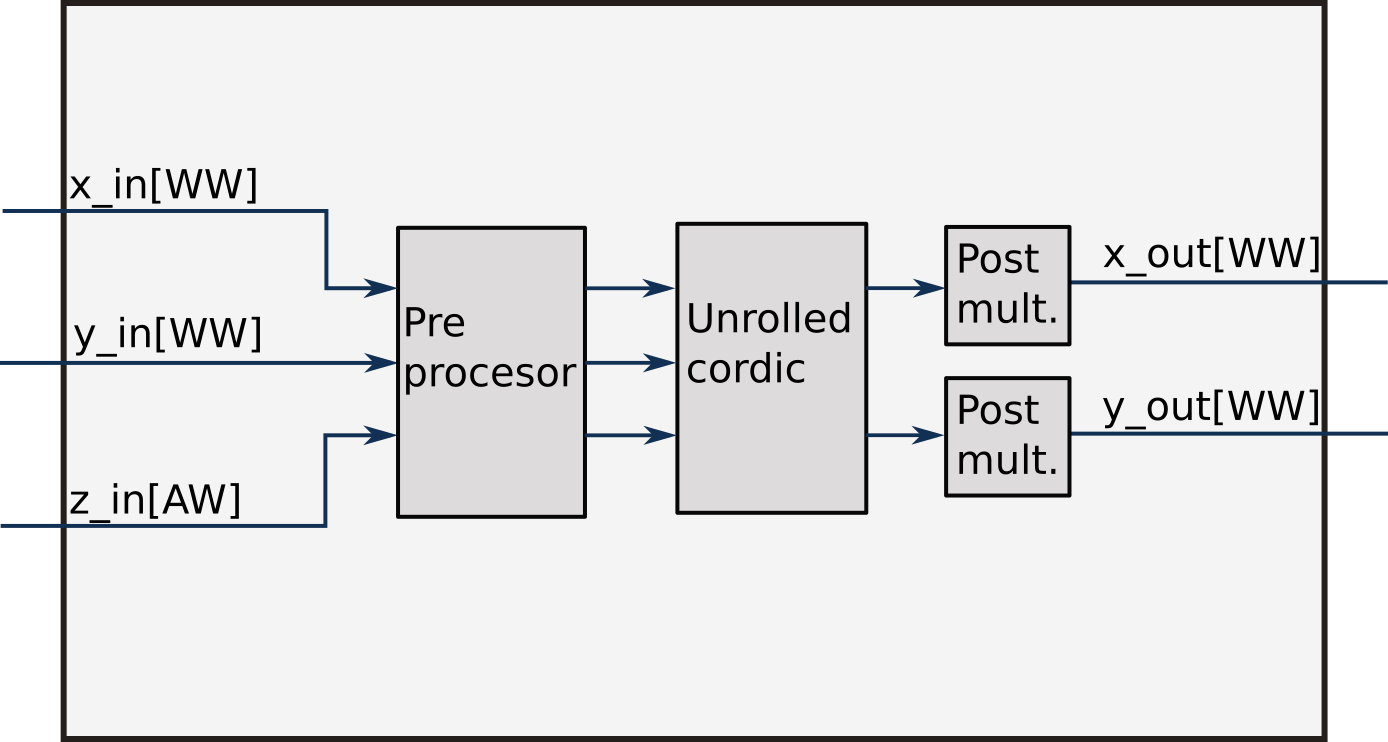
\includegraphics[width=9cm]{./figures/cordicBlocks.png}
        \caption{Diagrama en bloques del módulo cordic}
        \label{fig:cordicBlocks}
\end{figure}

\begin{figure}[htb!]
        \centering
        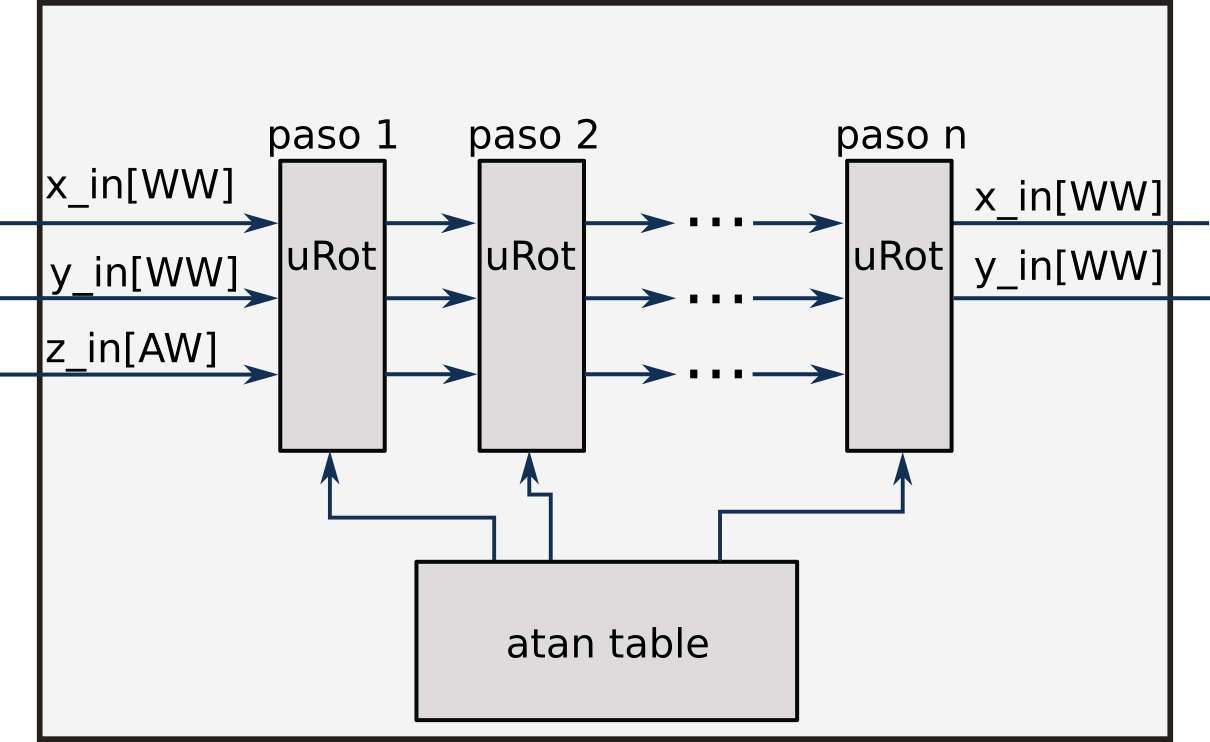
\includegraphics[width=9cm]{./figures/uCordicBlocks.png}
        \caption{Diagrama en bloques del bloque de rotaciones del módulo cordic}
        \label{fig:uCordicBlocks}
\end{figure}

Los bloques \textit{uRot} de la figura \ref{fig:uCordicBlocks} son los encargados de realizar las
microrotaciones sucesivas de acuerdo al algoritmo cordic. Los valores de los $\arctan(\alpha)$ se
almacenan previamente en la memoria \textit{atan table} de acuerdo a la cantidad de iteraciones que
se realizarán, y de allí son leídas por cada módulo de rotación.

\subsection{Multiplicador complejo}

La otra alternativa implementada para la multiplicación por los \textit{twiddle factors} es a través
de un multiplicador complejo. Para mantener la compatibilidad con el módulo cordic, y permitir que
la elección entre uno u otro sea transparente para el resto de las arquitecturas, se utilizan las
mismas interfaces en sus entradas y salidas, como se observa en la figura \ref{fig:multDiam}.

\begin{figure}[htb!]
        \centering
        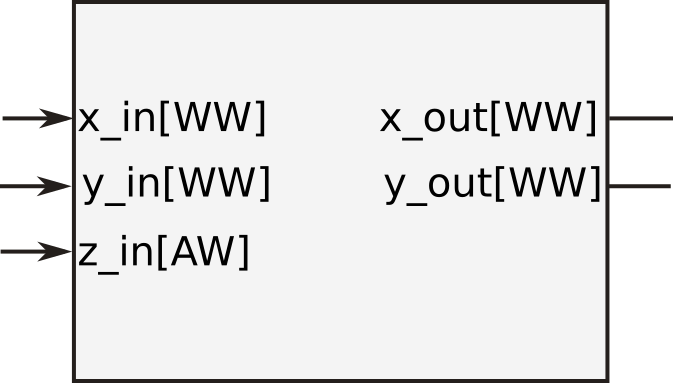
\includegraphics[width=7cm]{./figures/cordicDiam.png}
        \caption{Bloque de módulo multiplicador complejo}
        \label{fig:multDiam}
\end{figure}

El multiplicador recibe como entradas un vector de dos dimensiones, $x\_in$ e $y\_in$, y el ángulo
de rotación, $z\_in$, y entrega a las salidas el vector rotado en $x\_out$ e $y\_out$.

Para realizar la rotación a través de una multiplicación compleja, se almacenan los vectores
complejos correspondientes a cada ángulo posible de rotación en una memoria. Los vectores
almacenados tienen norma igual a $1$ de manera que no afecten la norma del vector de entrada.
Como los posibles ángulos de rotación son conocidos para una arquitectura y cantidad de puntos
dados, se ordenan en memoria de forma que esta sea direccionada por el valor del ángulo generado por
la unidad de control, obteniendo en cada posición el par de componentes del vector de norma $1$ que
corresponde al ángulo.\\
En la tabla \ref{table:angbits} se muestran ejemplos de la codificación binaria de
distintos ángulos para un ancho de palabra de ángulo de 7 bits.

\begin{table}[htb!]
\centering
\begin{tabular}{l c}
\textbf{Ángulo} & \textbf{Codificación binaria}\\ \hline 
$180^\circ$ & $100000$ \\
$90^\circ$ &  $0100000$ \\
$45^\circ$ &  $0010000$ \\
$135^\circ$ & $0110000$ \\ \hline
\end{tabular}
\caption{Ejemplos de codificación del ángulo para un ancho de palabra del ángulo de 7 bits}
\label{table:angbits}
\end{table}

Para reducir la cantidad de ángulos a almacenar se realiza un preprocesamiento previo donde se
analiza el ángulo y se realizan rotaciones iniciales en pasos de $90^\circ$ que consisten en intercambio
de las componentes y cambios de signo, que son operaciones triviales, y luego el ángulo restante
menor a $90^\circ$ se resuelve mediante la multiplicación compleja. De esta manera, en memoria solo deben
almacenarse ángulos menore a $90^\circ$.\\
Teniendo en cuenta que la variedad de ángulos a almacenar aumenta conforme aumenta la cantidad de
puntos para la que se instancia la arquitectura, y además esa variedad aumenta añadiendo ángulos de
tamaños cada vez menor, se implementa la tabla de forma que solo se crea del tamaño necesario para
la cantidad de puntos específica de la arquitectura particular que se está instanciando. Por ejemplo, para una arquitectura radix-2 de $16$ puntos, solo se necesita implementar la memoria con $4$
valores, incluyendo el ángulo $0$ en la posición de memoria $0$. En cambio para una radix-2 de $64$
puntos se necesitan $32$ valores de ángulos distintos almacenados en memoria.\\

Para direccionarlos se utiliza la palabra del ángulo trasladado al primer cuadrante invertida, de
modo que la posición de memoria correspondiente al ángulo $0$ es la $0$, la corresponfiente al
ángulo $45^\circ$ ($10\ldots0$) es la $1$ ($00\ldots01$), y así sucesivamente.\\

Al utilizar una transformación del ángulo a su vector normalizado correspondiente, no es necesario
un escalamiento luego de multiplicar.

\subsection{Unidad de escalamiento} \label{sec:secEscal}

La unidad de escalamiento de las unidades aritméticas de cada arquitectura permite realizar un
escalamiento del resultado de la operación aritmética en una o varias etapas seleccionadas en forma
dinámica, mediante una señal de entrada, para evitar posibles \textit{overflow} a lo largo del
cómputo de la FFT, ya que la aritmética de la arquitectura es de punto fijo en palabras de longitud
fija.\\

Las opciones de escalamiento disponibles, como se explicó en la subsección \ref{sec:redond}, son
redondeo y truncamiento.

En la figura \ref{fig:escBlocks} se muestra el diagrama en bloques de la unidad de escalamiento.

\begin{figure}[htb!]
        \centering
        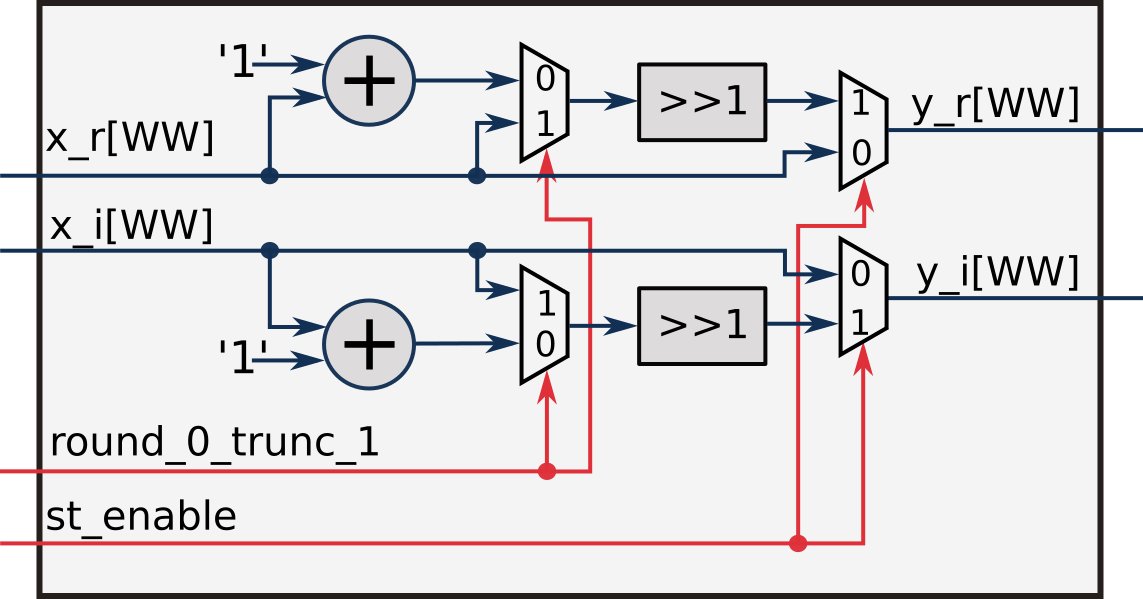
\includegraphics[width=9cm]{./figures/escBlocks.png}
        \caption{Diagrama en bloques de la unidad de escalamiento}
        \label{fig:escBlocks}
\end{figure}

La unidad le suma $1$ a cada una de las entradas. Con un multiplexor controlado por la señal
\textit{round\_0\_trunc\_1} se elige si se desplaza a derecha un bit la señal original o la salida
del sumador, eligiendo así entre truncamiento o redondeo respectivamente. Luego, la salida de la unidad
será la seña original, en caso de no estar habilitado el escalamiento para esa etapa, o la señal
desplazada, en caso de estar habilitado el escalamiento para esa etapa, realizando la selección
mediante dos multilpexores controlados por la señal \textit{st\_enable}.

\section{Interfaces de las arquitecturas}

Las dos arquitecturas implementadas tienen los mismos puertos de entrada y salida mostrados en la
figura \ref{fig:arqInterf}. 

\begin{figure}[htb!]
        \centering
        \includegraphics[width=8cm]{./figures/arcInterf.png}
        \caption{Señales de comunicación de las arquitecturas implementadas}
        \label{fig:arqInterf}
\end{figure}

Los puertos se describen en el siguiente listado:

\begin{itemize}
  \item \textbf{x\_real} ($WORD\_WIDTH$) componente real del punto de entrada.
  \item \textbf{x\_imag} ($WORD\_WIDTH$) componente imaginaria del punto de entrada.
  \item \textbf{arst} señal de reset asincrónico. Reinicia la arquitectura.
  \item \textbf{start} Señal de comienzo de funcionamiento luego de un reinicio. Al detectar la
  señal la arquitectura lee el primer dato de entrada y comienza con el cómputo de la primer FFT.
  \item \textbf{st\_scale\_en} ($(\log_\nu(N)))$) Habilitación del escalamiento posterior a la
  operación aritmética. Un $'1'$ en un bit habilita el escalamiento en la etapa correspondiente.
  \item \textbf{round\_0\_trunc\_1} Selección del tipo de escalamiento posterior a la operación
  aritmética, redondeo o truncamiento.
  \item \textbf{y\_real} ($WORD\_WIDTH$) componente real del punto de salida.
  \item \textbf{y\_imag} ($WORD\_WIDTH$) componente imaginaria del punto de salida.
  \item \textbf{rfd} señal que indica que debe colocarse un nuevo punto en la entrada de la
  arquitectura.
  \item \textbf{data\_valid} señal que indica que el dato presente en la salida es válido.
  \item \textbf{soo} señal que indica que el dato presente en la salida es el primero de una nueva
  FFT.
  \item \textbf{done} señal que indica que el dato presente en la salida es el último de la actual
  FFT.
\end{itemize}

Se listan a continuación los parámetros globales de las arquitecturas implementadas.

\begin{itemize}
  \item \textbf{WORD\_WIDTH} Cantidad de bits de codificación de los puntos de entrada y salida.
  \item \textbf{CLOG2\_FFT\_POINTS} Logaritmo, en base dos, de la cantidad de puntos para la que es
  implementada la arquitectura. A través de este parámetro se infiere dentro de la arquitectura la
  cantidad de puntos de la FFT a procesar.
  \item \textbf{FFT\_1\_IFFT\_0} selección de implementación de la arquitectura para realizar FFT o
  IFFT.
  \item \textbf{ANGLE\_WIDTH} Cantidad de bits de codificación de los ángulos de representación de
  los \textit{twiddle factors}.
\end{itemize}

\section{Herramientas utilizadas para el desarrollo} \label{sec:herrSec}
% En el capítulo anterior se analizaron diferentes tipos de arquitecturas existentes para la implementación de un procesador de descomposición QR. Se describieron sus características a nivel conceptual y se detallaron las definiciones de la implementación elegida para realizar la implementación.
% 
% En este capítulo se describen las herramientas que fueron utilizadas y se explica en detalle, a nivel de microarquitectura, la forma en la cual fue implementado cada módulo del procesador desarrollado, y la forma en la cual los módulos son interconectados para conformar al mismo. Adicionalmente, se describen aquellas definiciones y desarrollos que fueron el resultado de la presente tesis, utilizados para resolver diferentes necesidades encontradas, los cuales representan un contenido intelectual propio.
% 
% La metodología utilizada para el desarrollo del procesador consistió en analizar las necesidades de la arquitectura elegida, y los diferentes componentes requeridos. Se procedió a la definición de dicha arquitectura a través de un diagrama en bloques y se desarrolló cada uno de los módulos por separado, gradualmente. Una vez desarrollado un módulo, se procedíó a simular su comportamiento aislado a través de un testbench que lograra contemplar la mayor parte de los posibles vectores de entrada. Una vez finalizada la simulación individual de los distintos componentes, se procedó a realizar una simulación conjunta de algunos de ellos.
% 
% \section{Herramientas utilizadas}
% 
 A continuación se hace una breve reseña de las herramientas utilizadas para la implementación de
 las arquitecturas:
 
\subsubsection*{Sublime Text 2}
\begin{wrapfigure}{r}{0.22\textwidth}
	\vspace{-15pt}
	\begin{center}
		\includegraphics[width=0.20\textwidth]{./figures/logo_sublime.png}
	\end{center}
	\vspace{-15pt}
\end{wrapfigure}
Sublime fue el editor de texto utilizado para codificar en lenguaje Verilog. El mismo presenta una
interfaz gráfica con diferentes características de gran utilidad, marcado de palabras claves,
autocompletado, etc.

% \subsubsection*{Vim}
% \begin{wrapfigure}{r}{0.22\textwidth}
% 	\vspace{-20pt}
% 	\begin{center}
% 		\includegraphics[width=0.15\textwidth]{./figures/logo_vim.png}
% 	\end{center}
% 	\vspace{-20pt}
% \end{wrapfigure}
% Vim es un editor de texto nativo de entornos de tipo UNIX y fue utilizado en algunos casos en conjunto con Sublime Text 2.
% 
\subsubsection*{ModelSim}
\begin{wrapfigure}{r}{0.22\textwidth}
	\vspace{-15pt}
	\begin{center}
		\includegraphics[width=0.20\textwidth]{./figures/logo_modelsim.png}
	\end{center}
	\vspace{-15pt}
\end{wrapfigure}
ModelSim fue la herramienta utilizada para la simulación de los códigos descriptos en Verilog, con
los cuales se generaron archivos de tipo wave de salida.

\subsubsection*{gtkwave}
\begin{wrapfigure}{r}{0.22\textwidth}
	\vspace{-15pt}
	\begin{center}
		\includegraphics[width=0.20\textwidth]{./figures/logo_gtkwave.png}
	\end{center}
	\vspace{-15pt}
\end{wrapfigure}
Gtkwave fue la herramienta utilizada para visualizar los archivos de tipo wave que fueron generados
durante las simulaciones realizadas en ModelSim.

\subsubsection*{Xilinx ISE}
\begin{wrapfigure}{r}{0.22\textwidth}
	\vspace{-15pt}
	\begin{center}
		\includegraphics[width=0.15\textwidth]{./figures/logo_ise.png}
	\end{center}
	\vspace{-15pt}
\end{wrapfigure}
Xilinx ISE es la herramienta proporcionada por la compañía Xilinx para crear los archivos de
síntesis ``.bit'' a partir de un hardware codificado en un lenguaje HDL, para ser implementado en
los dispositivos FPGA que provee. También fue utilizada para transferir los archivos ``.bit'' al
kit de desarrollo FPGA.

\subsubsection*{Bitbucket/Mercurial}
\begin{wrapfigure}{r}{0.22\textwidth}
	\vspace{-15pt}
	\begin{center}
		\includegraphics[width=0.20\textwidth]{./figures/logo_bitbucket.png}
	\end{center}
	\vspace{-15pt}
\end{wrapfigure}
Para realizar el desarrollo se utilizó un repositorio hospedado en
\href{http://www.bitbucket.org}{http://www.bitbucket.org}, el cual fue utilizado a través de la
herramienta de versionado Mercurial. Dicho sistema aportó diversas ventajas, entre las cuales
principalmente se encuentran el mantener un registro de todas las modificaciones realizadas entre
cada una de las versiones y el poder trabajar en la nube.
 
\chapter{Estudio, Simulación y Validación de los IP Cores Generados} \label{sec:simsec}

En este capítulo se describen los ensayos de verificación y validación de los IP
Cores generados durante el desarrollo del presente trabajo de tesis. 

\section{Estrategia de simulación, verificación y validación}

Durante el desarrollo de este trabajo se verificó el funcionamiento de cada módulo a través de
simulaciones en verilog comprobando su correcto funcionamiento.

Dada la imposibilidad de ensayar todos los casos, por temas de tiempo, se diseñaron casos de prueba
específicos que son una muestra representativa del conjunto total.

Una vez integrada cada arquitectura se realizaron ensayos de verificación y validación. Mediante
bancos de prueba en verilog se procesaron señales características y se compararon con el resultado de
realizar el mismo procesamiento utilizando Matlab para comprobar el correcto funcionamiento de las
arquitecturas finalizadas. 

Para caracterizar las diferentes arquitecturas se eligieron las siguientes métricas:

\begin{itemize}
  \item Error máximo $\equiv$ $\Vert error \Vert_\infty$
  \item MSE $\equiv$ $\Vert error \Vert_2$
  \item Distorsión Total Armónica
\end{itemize} 

Una vez verificado el funcionamiento a nivel general corroborando que transforma señales conocidas
en sus transformadas y antitransformadas correspondientes, se realizaron ensayos de caracterización
mediante simulaciones a través de bancos de prueba en verilog donde se analizó iterativamente el
funcionamiento de las arquitecturas para obtener parámetros de caracterización como la distorsión
total armónica y una métrica del error de la arquitectura tomando como referencia el procesamiento
de las mismas señales en Matlab.

Se realizaron simulaciones para diferentes tamaños de palabra y cantidad de puntos. Para la cantidad
de bits por palabra se utilizaron los valores de 12 y 16 bits. Estos valores fueron seleccionados
teniendo en cuenta por un lado que 16 bits es un valor standard de codificación y permite la comparación
directa con unidades de cómputo en otros lenguajes como C++, y 12 bits por ser un valor común en lo
que se refiere a transmisiones OFDM. En cuanto a la cantidad de puntos a procesar se realizaron
simmulaciones para $1024$ y $4096$ puntos, al ser cantidades de puntos que pueden procesarse tanto
con la arquitectura radix-2 como con la radix-4.

Todas las simulaciones fueron realizadas utilizando \textit{Modelsim} y \textit{gtkwave}, ambos
mencionados en la sección \ref{sec:herrSec}, para la visualización de las señales resultantes.

\section{Simulación y verificación de los módulos individuales}

Al finalizar la implementación de cada módulo se realizaron pruebas elementales de funcionamiento
utilizando bancos de prueba escritos en verilog donde se buscó verificar que cada módulo cumpla con su
función.

En este sentido los módulos sobre los que se realizaron mayores pruebas son los módulos
multiplicadores, tanto el módulo cordic como el multiplicador complejo.
También se realizaron ensayos de funcionamiento durante el desarrollo de las unidades de control
para depurar la sincornización correcta de las señales de control.

Una vez finalizados los
ensayos y simulaciones con resultados satisfactorios se procedió a la integración de las
arquitecturas.

\section{Simulación y validación de las arquitecturas completas}

Los IP cores generados como resultado del desarrollo del trabajo de tesis fueron sometidos a
simulaciones y ensayos para verificar su correcto funcionamiento de acuerdo a los requerimientos
planteados y obtener cotas de error y distorsión para validar el desarrollo.

\subsection{Procesamiento de señales patrón} \label{sec:enspatron}

Se realizaron una serie de simulaciones utilizando señales patrón cuyas transformadas de Fourier son
conocidas de forma de validar el funcionamiento de las arquitecturas. Para cada señal utilizada se
presenta un gráfico con el resultado de la simulación superpuesto al resultado de realizar la
transformada de Fourier sobre la misma señal utilizando Matlab.
Las arquitecturas se ensayan utilizando un ancho de palabra de $16$ bits, para $4096$ puntos.

\subsubsection{Delta en componente `0'}

Utilizando como entrada una señal compuesta por un único pulso en la primer posición debe dar como
resultado una señal continua de valor constante.

La entrada consistió en
una señal discreta de $4096$ puntos representando el muestreo de una delta en la componente $0$.

En la figura \ref{fig:outDelta0} se observan las salidas obtenidas utilizando ambas arquitecturas
tanto con el multiplicador complejo como con el rotador cordic. En cada gráfico se superpone la
salida de la arquitectura, representada por la señal \textit{core} en los gráficos, a la salida de
realizar la misma fft utilizando precisión de punto flotante como referencia.

\begin{figure}[htbp!]
        %\centering
        \advance\leftskip-1.5cm
        \begin{subfigure}{0.6\textwidth}
        \includegraphics[width=9cm]{./figures/r2_delta0_16_4096_mul.png}
        \caption{Radix 2, multiplicador complejo}
        \end{subfigure}%
        \begin{subfigure}{0.6\textwidth}%\centering
        \includegraphics[width=9cm]{./figures/r2_delta0_16_4096_cor.png}
        \caption{Radix 2, rotador cordic}
        \end{subfigure} 
        \begin{subfigure}{0.6\textwidth}%\centering
        \includegraphics[width=9cm]{./figures/r4_delta0_16_4096_mul.png}
        \caption{Radix 4, multiplicador complejo}
        \end{subfigure}%
        \begin{subfigure}{0.6\textwidth}%\centering
        \includegraphics[width=9cm]{./figures/r4_delta0_16_4096_cor.png}
        \caption{Radix 4, rotador cordic}
        \end{subfigure}
        \caption{Respuestas a una delta en la componente $0$ para las arquitecturas radix-2 y
        radix-4}
        \label{fig:outDelta0}
\end{figure}

\subsubsection{Delta}

La transformada de Fourier de una delta debe dar un seno o un coseno cuya frecuencia está
directamente relacionada con la posición del pulso.

La entrada utilizada para este ensayo consistió en
una delta ubicada en la componente $6$ del vector de $4094$ puntos.

En la figura \ref{fig:outDelta7} se muestran las salidas obtenidas de ambas arquitecturas tanto con
el multiplicador complejo como el rotador cordic. En cada gráfico se superpone la
salida de la arquitectura, representada por la señal \textit{core} en los gráficos, a la salida de
realizar la misma fft utilizando precisión de punto flotante como referencia.

\begin{figure}[htbp!]
        %\centering
        \advance\leftskip-1.5cm
        \begin{subfigure}{0.6\textwidth}
        \includegraphics[width=9cm]{./figures/r2_delta7_16_4096_mul.png}
        \caption{Radix 2, multiplicador complejo}
        \end{subfigure}%
        \begin{subfigure}{0.6\textwidth}%\centering
        \includegraphics[width=9cm]{./figures/r2_delta7_16_4096_cor.png}
        \caption{Radix 2, rotador cordic}
        \end{subfigure} 
        \begin{subfigure}{0.6\textwidth}%\centering
        \includegraphics[width=9cm]{./figures/r4_delta7_16_4096_mul.png}
        \caption{Radix 4, multiplicador complejo}
        \end{subfigure}%
        \begin{subfigure}{0.6\textwidth}%\centering
        \includegraphics[width=9cm]{./figures/r4_delta7_16_4096_cor.png}
        \caption{Radix 4, rotador cordic}
        \end{subfigure}
        \caption{Respuestas a una delta en la componente $7$ para las arquitecturas radix-2 y
        radix-4}
        \label{fig:outDelta7}
\end{figure}

\subsection{Medición del error}

Para medir el error de procesamiento de las arquitecturas se utilizó como parámetro el resultado de
realizar el mismo procesamiento mediante Matlab, ya que al utilizar precisión en punto flotante de
64 bits provee un buen contraste para la precisión en entero de 12 o 16 bits de las arquitecturas.

Para obtener un parámetro comparable del error
se obtienen dos métricas basadas en el cálculo de la norma de los vectores de señal y de error.
Definiendo la norma $p$ de un vector $x$ de tamaño $N$ como:

\begin{equation}
\Vert\vec{x}\Vert_p = \sqrt[p]{x[1]^p+x[2]^p+\ldots+x[N]^p}
\label{eq:normap}
\end{equation}

Se toma el error relativo en base a dos normas calculadas según (\ref{eq:normap}), dando las
métricas $E_\infty$ y $E_2$ como sigue:

\begin{equation}
E_\infty = MAX\left(\frac{ X_o[n] - X_{dut}[n]}{X_o[n]}\right)
\label{eq:norma1}
\end{equation}

\begin{equation}
E_2 = \left\Vert\frac{X_o[n] - X_{dut}[n]}{X_o[n]}\right\Vert_2
\label{eq:norma2}
\end{equation}

permitiendo estas métricas tener una medida del error ponderable y comparable.

Teniendo en cuenta que las arquitecturas implementadas se comportan como sistemas no lineales, para
obtener métricas confiables de error cada simulación consistió en $1024$ corridas con vectores de
entrada generados aleatoriamente en cada corrida. Se calcularon las métricas $E_\infty$ y $E_2$ para
cada corrida y luego se promedió el valor de las métricas de todas las corridas obteniendo así los
valores de error de cada simulación.

En la figura \ref{fig:errorsim} se presenta un diagrama de flujo del \textit{script} de simulación para la
estimación del error. 

\begin{figure}[htb!]
        \centering
        \includegraphics[width=4cm]{./figures/error_sim.png}
        \caption{Diagrama de flujo de la simulación para la estimación del error}
        \label{fig:errorsim}
\end{figure}

Se simularon $8$ esquemas distintos para cada arquitectura, donde se alternaron los dos módulos
multiplicadores, la unidad cordic y el multiplicador complejo, con dos anchos de palabra, $12$ y
$16$ bits, para dos cantidades de puntos diferentes, $1024$ y $4096$.
Además se realizaron dos simulaciones más utilizando una unidad de cómputo de FFT desarrollada por
terceros ampliamente difundida en lenguaje C++, conocida como KISS FFT \cite{KISSFFT},
con precisión de punto fijo de 16 bits.
%TODO métrica s de error

En la tabla \ref{table:errorInf} se muestran los resultados de las mediciones de error utilizando la
métrica $E_\infty$, mientras que en la tabla \ref{table:error2} se muestran las mediciones de error
utilizando la métrica $E_2$.

\begin{table}[htb!]
\begin{tabular}{l c c c c}
 & \textbf{1024, 12 bits} & \textbf{1024, 16 bits} & \textbf{4096, 12 bits} & \textbf{4096, 16 bits}\\ \hline 
\textbf{Radix-2, cordic} & $0.092$ & $0.006$ & $0.099$ & $0.008 $\\
\textbf{Radix-2, Mult.} & $0.232$ & $0.003$ & $0.340$ & $0.108$\\
\textbf{Radix-4, cordic} & $0.077$ & $0.003$ & $0.074$ & $0.007$\\
\textbf{Radix-4, Mult.} & $0.224$ & $0.002$ & $0.334$ & $0.105$\\
\textbf{Kiss FFT} & $ $ & $0.017$ & $ $ & $0.035$\\\hline
\end{tabular}
\caption{Métrica $E_\infty$ para 1024 realizaciones de cada arquitectura con entradas aleatorias}
\label{table:errorInf}
\end{table}

\begin{table}[htb!]
\begin{tabular}{l c c c c }
 & \textbf{1024, 12 bits} & \textbf{1024, 16 bits} & \textbf{4096, 12 bits} & \textbf{4096, 16 bits}\\ \hline 
\textbf{Radix-2, cordic} & $0.095$ & $0.007$ & $0.116$ & $0.053$\\
\textbf{Radix-2, Mult.} & $0.257$ & $0.004$ & $0.356$ & $0.131$\\
\textbf{Radix-4, cordic} & $0.084$ & $0.002$ & $0.094$ & $0.027$\\
\textbf{Radix-4, Mult.} & $0.258$ & $0.003$ & $0.358$ & $0.126$\\ 
\textbf{Kiss FFT} & $ $ & $0.017$ & $ $ & $0.035$\\\hline
\end{tabular}
\caption{Métrica $E_2$ para 1024 corridas de cada arquitectura con entradas aleatorias}
\label{table:error2}
\end{table}

Se puede ver que el desempeño de las distintas variantes de las arquitecturas es aceptable, incluso
comparado con el algoritmo FFT implementado en C++.

Se puede ver que para $12$ bits el algoritmo cordic produce menor error que el multiplicador
complejo. Esto se debe a que el efecto de la cuantización se hace más evidente en el multiplicador
ya que al implementar los factores de multiplicación correspondientes a cada ángulo, el error de
cuantización es mayor que al utilizar solo el ángulo como en el caso del cordic. Además, el hecho de
realizar una multiplicación entre dos valores con precisión de punto fijo el error del resultado es
mayor que en el caso de sumas y dezplazamientos de una sola palabra como sucede en el cordic.
En cambio, para un tamaño de palabra de $16$ bits la magnitud del error de ambos sistemas de
multiplicación por los twiddle factors es equivalente ya que es menos significativo el error de
cuantización de los factores del multiplicador.

Para reducir el error del multiplicador complejo se debe
aumentar el tamaño de palabra con el que se almacenan los factores correspondientes a cada ángulo,
lo que aumenta el tamaño de memoria utilizada y el tamaño de los registros con los que se realizan
las operaciones. Para reducir el error del rotador cordic se puede aumentar la cantidad de
iteraciones del algoritmo, pero esto tiene como concecuencia un aunmento en el tiempo consumido para
realizar la rotación y un aumento en la memoria destinada a almacenar los valores de
$\arctan(2^{-i})$.

Tambien se puede observar que el error para las arquitecturas de $4096$ puntos es mayor que el error
para las arquitecturas de $1024$ puntos. Esto se debe a que para procesar mayor cantidad de puntos
se requiere mayor cantidad de etapas, lo que lleva a mayor cantidad de operaciones aritméticas que
contienen error, que se acumula y se arrastra de una etapa a la siguiente. De este modo, mientras
más etapas tenga la arquitectura mayor será el error de la misma. Por este mismo motivo las
arquitecturas radix-4 presentan menor error que las radix-2, ya que para la misma cantidad de
puntos poseen menor número de etapas, lo que resulta en menos multiplicaciones. Esto último
representa la principal ventaja de la arquitectura radix-4 por sobre la radix-2 indepenientemente
del tipo de implementación que se utilice.

La diferencia en el error para los dos tamaños de palabras ensayados se debe al error de
cuantización producto de la diferencia de precisión entre los dos tamaños. Mientras que con
$12$ bits la cuantización se da en pasos de $\frac{1}{2^{12-1}} = 4.88 * 10^{-4}$, para $16$ bits es
de $\frac{1}{2^{16-1}} = 3.05 * 10^{-5}$.

También se observa que para $1024$ puntos el error de las arquitecturas iterativas es menor que el
de la Kiss FFT, mientras que para $4096$ puntos el error de las arquitecturas utilizando cordic es
del orden del error de la implementación en C++. Estos resultados verifican que las arquitecturas
resultantes del presente trabajo de tesis son aptas para su uso práctico, al menos en cuanto al
error que producen.\\ 
En cuanto a los resultados de error para las arquitecturas con multiplicador
complejo de $4096$ puntos, se debería aumentar el ancho de palabra de los factores de multiplicación
almacenados en memoria para mejorar las métricas obtenidas.


\subsection{Medición de la distorsión total armónica}

La distorsión total armónica (THD por sus siglas en inglés, Total Harmonic Distortion) es
la aparición de componentes espúreas en la salida de un sistema no lineal al aplicar a la entrada un
tono puro.
En el caso del presente trabajo de tesis el procesamiento de
datos comprende el cómputo de una FFT o iFFT, por lo que la aparición de componentes espúreas tanto en frecuencia como en muestras
temporales debe mantenerse en el nivel míinimo posible ya que puede distorisonar completamente el
resultado del procesamiento, además de ser una medida de la no linealidad del sistema.

La distorsión total armónica se calcula como:

\begin{equation}
THD = \frac{\sum Potencia de los armonicos}{Potencia del tono fundamental} =
\frac{P_1+P_2+\ldots +P_N}{P_0}
\label{eq:THD1}
\end{equation}

Donde $P_0$ es la potencia del tono fundamental de frecuencia $f_0$ y $P_1\ldots P_N$ la potencia de
los armónicos de frecuencia $2*f_0\ldots N*f_0$.

Para obtener una caracterización de la \textit{THD} se utilizó un banco de prueba en verilog que permite
leer como entrada valores complejos listados en un archivo de texto, realizar el cómputo de la FFT
mediante la arquitectura a ensayar y escribir la salida en un archivo de texto. 
La simulación completa se llevó a cabo mediante un \textit{script} en Matlab que crea un archivo de texto que
funciona como entrada de la arquitectura, llama a la simulación de la arquitectura mediante el
banco de prueba descripto y luego procesa la salida de la simulación para hallar el valor de la
\textit{THD}, realizando su transformada de Fourier en un sistema de mayor precisión y analizando
sus componentes.
Para lograr una caracterización lo más completa posible se realizaron simulaciones sucesivas recorriendo de a uno por vez todos los tonos de entrada posibles y registrando el valor de
\textit{THD} para cada uno, de forma de obtener el valor para cada tono de entrada.\\
La forma de calcular la \textit{THD} es la siguiente:

\begin{equation}
THD = 10*\log(\frac{\sum_1^N A_i^2}{A_0^2})
\label{eq:THD2}
\end{equation}

donde $A_i$ es la amplitud de la componente de frecuencia $f_i$, dando el resultado del cálculo en
dB.

En la figura \ref{fig:thdsim} se muestra un diagrama de flujo de la simulación para la estimación de
la \textit{THD}. \textit{Core sim} indica la simulación del IP Core mediante Modelsim, el resto de
las acciones son llevadas a cabo en Matlab.

\begin{figure}[htb!]
        \centering
        \includegraphics[width=4cm]{./figures/thd_sim.png}
        \caption{Diagrama de flujo de la simulación para la estimación de la THD}
        \label{fig:thdsim}
\end{figure}

De este modo se llevaron a cabo 16 simulaciones, combinando los dos valores de tamaño de palabra y
los dos valores de cantidad de puntos, para cada una de las dos arquitecturas desarrolladas
utilizando como unidad de multiplicación por los \textit{twiddle factors} el módulo cordic y el
multiplicador complejo. Además se realizó el mismo análisis para una arquitectura KISS FFT utilizando tamaño de
palabra de 16 bits en punto fijo.
% En las tablas \ref{table:THDprom12} y \ref{table:THDprom16} se muestran la distorsión armónica total 
% promedio para cada una de las configuraciones mencionadas para cada arquitectura separadas por
% tamaño de palabra. El promedio mostrado en dichas tablas se obtuvo descartando los tonos que al ser
% procesados dieron un valor de \textit{THD} interpretado por Matlab como $-\infty$, valor debido al
% que el valor de magnitud de los armónicos es cero.
% 
% \begin{table}[htb!]
% \begin{tabular}{l c c c c}
%  & \textbf{Radix-2 cordic} & \textbf{Radix-2 mult} & \textbf{Radix-4 cord} & \textbf{Radix-4 mult}\\ \hline 
% \textbf{1024 puntos} & $-69.68$ & $-85.84$ & $-70.52$ & $-84.1$\\
% \textbf{4096 puntos} & $-76.51$ & $ -92.23$ & $-77.31$ & $-90.08$\\ \hline
% \end{tabular}
% \caption{THD promedio para tamaño de palabra de 12 bits}
% \label{table:THDprom12}
% \end{table}
% 
% %TODO Modificar tabla con resultados de simulación:
%  \begin{table}[htb!]
% \begin{tabular}{l c c c c c}
% & \textbf{R-2 cordic} & \textbf{R-2 mult} & \textbf{R-4 cordic} & \textbf{R-4 mult} &
% \textbf{Kiss-FFT}\\ \hline
% \textbf{1024 puntos} & $ $ & $-108.72$ & $-92.37$ & $ $ & $-59.48$\\
% \textbf{4096 puntos} & $ $ & $-116.98$ & $ $ & $-116.88 $ & $-52.95$\\ \hline
% \end{tabular}
% \caption{THD promedio para tamaño de palabra de 16 bits}
% \label{table:THDprom16}
% \end{table}

En la figura \ref{fig:r2_thd_1024} se muestra la THD para cada tono utilizado como
entrada, para la arquitectura radix-2 iterativa para 1024 puntos, tanto para 12 bits como para 16 bits de
ancho de palabra, utilizando el rotador cordic y el multiplicador complejo.

\begin{figure}[htbp!]
        %\centering
        \advance\leftskip-1.5cm
        \begin{subfigure}{0.6\textwidth}%\centering
        \includegraphics[width=9cm]{./figures/thd_r2_1024_12_mul.png}
        \caption{Radix 2, multiplicador complejo, 12 bits}
        \end{subfigure}%
        \begin{subfigure}{0.6\textwidth}\centering
        \includegraphics[width=9cm]{./figures/thd_r2_1024_12_cor.png}
        \caption{Radix 2, rotador cordic, 12 bits}
        \end{subfigure} 
        \begin{subfigure}{0.6\textwidth}\centering
        \includegraphics[width=9cm]{./figures/thd_r2_1024_16_mul.png}
        \caption{Radix 2, multiplicador complejo, 16 bits}
        \end{subfigure}% 
        \begin{subfigure}{0.6\textwidth}\centering
        \includegraphics[width=9cm]{./figures/thd_r2_1024_16_cor.png}
        \caption{Radix 2, rotador cordic, 16 bits}
        \end{subfigure}%
        \caption{THD en función del tono de entrada, radix-2 de 1024 puntos}
        \label{fig:r2_thd_1024}
\end{figure}

En la figura \ref{fig:r2_thd_4096} se ven los gráficos de la THD para cada tono utilizado como
entrada, para la arquitectura radix-2 iterativa para 4096 puntos, tanto para 12 bits como para 16 bits de
ancho de palabra, utilizando el rotador cordic y el multiplicador complejo.

\begin{figure}[htbp!]
        %\centering
        \advance\leftskip-1.5cm
        \begin{subfigure}{0.6\textwidth}%\centering
        \includegraphics[width=9cm]{./figures/thd_r2_4096_12_mul.png}
        \caption{Radix 2, multiplicador complejo, 12 bits}
        \end{subfigure}%
        \begin{subfigure}{0.6\textwidth}%\centering
        \includegraphics[width=9cm]{./figures/thd_r2_4096_12_cor.png}
        \caption{Radix 2, rotador cordic, 12 bits}
        \end{subfigure} 
        \begin{subfigure}{0.6\textwidth}%\centering
        \includegraphics[width=9cm]{./figures/thd_r2_4096_16_mul.png}
        \caption{Radix 2, multiplicador complejo, 16 bits}
        \end{subfigure}% 
        \begin{subfigure}{0.6\textwidth}%\centering
        \includegraphics[width=9cm]{./figures/thd_r2_4096_16_cor.png}
        \caption{Radix 2, rotador cordic, 16 bits}
        \end{subfigure} 
        \caption{THD en función del tono de entrada, radix-2 de 4096 puntos}
        \label{fig:r2_thd_4096}
\end{figure}

En la figura \ref{fig:r4_thd_1024} se ven los gráficos de la THD para cada tono utilizado como
entrada, para la arquitectura radix-4 iterativa para 1024 puntos, tanto para 12 bits como para 16 bits de
ancho de palabra, utilizando el rotador cordic y el multiplicador complejo.

\begin{figure}[htbp!]
        %\centering
        \advance\leftskip-1.5cm
        \begin{subfigure}{0.6\textwidth}%\centering
        \includegraphics[width=9cm]{./figures/thd_r4_1024_12_mul.png}
        \caption{Radix 4, multiplicador complejo, 12 bits}
        \end{subfigure}%
        \begin{subfigure}{0.6\textwidth}%\centering
        \includegraphics[width=9cm]{./figures/thd_r4_1024_12_cor.png}
        \caption{Radix 4, rotador cordic, 12 bits}
        \end{subfigure} 
        \begin{subfigure}{0.6\textwidth}%\centering
        \includegraphics[width=9cm]{./figures/thd_r4_1024_16_mul.png}
        \caption{Radix 4, multiplicador complejo, 16 bits}
        \end{subfigure}% 
        \begin{subfigure}{0.6\textwidth}%\centering
        \includegraphics[width=9cm]{./figures/thd_r4_1024_16_cor.png}
        \caption{Radix 4, rotador cordic, 16 bits}
        \end{subfigure} 
        \caption{THD en función del tono de entrada, radix-4 de 1024 puntos}
        \label{fig:r4_thd_1024}
\end{figure}

En la figura \ref{fig:r4_thd_4096} se ven los gráficos de la THD para cada tono utilizado como
entrada, para la arquitectura radix-4 iterativa para 4096 puntos, tanto para 12 bits como para 16 bits de
ancho de palabra, utilizando el rotador cordic y el multiplicador complejo.

\begin{figure}[htbp!]
        %\centering
        \advance\leftskip-1.5cm
        \begin{subfigure}{0.6\textwidth}%\centering
        \includegraphics[width=9cm]{./figures/thd_r4_4096_12_mul.png}
        \caption{Radix 4, multiplicador complejo, 12 bits}
        \end{subfigure}%
        \begin{subfigure}{0.6\textwidth}%\centering
        \includegraphics[width=9cm]{./figures/thd_r4_4096_12_cor.png}
        \caption{Radix 4, rotador cordic, 12 bits}
        \end{subfigure} 
        \begin{subfigure}{0.6\textwidth}%\centering
        \includegraphics[width=9cm]{./figures/thd_r4_4096_16_mul.png}
        \caption{Radix 4, multiplicador complejo, 16 bits}
        \end{subfigure}% 
        \begin{subfigure}{0.6\textwidth}%\centering
        \includegraphics[width=9cm]{./figures/thd_r4_4096_16_cor.png}
        \caption{Radix 4, rotador cordic, 16 bits}
        \end{subfigure} 
        \caption{THD en función del tono de entrada, radix-4 de 4096 puntos}
        \label{fig:r4_thd_4096}
\end{figure}

En la figura \ref{fig:kiss_thd_4096} se ven los gráficos de la THD para cada tono utilizado como
entrada, para la arquitectura KISS FFT en C++ para 16 bits de
ancho de palabra, para 1024 y 4096 puntos.

\begin{figure}[htbp!]
        %\centering
        \advance\leftskip-1.5cm
        \begin{subfigure}{0.6\textwidth}%\centering
        \includegraphics[width=9cm]{./figures/thd_kiss_1024_16.png}
        \caption{Kiss FFT, 1024 puntos}
        \end{subfigure}% 
        \begin{subfigure}{0.6\textwidth}%\centering
        \includegraphics[width=9cm]{./figures/thd_kiss_4096_16.png}
        \caption{Kiss FFT, 4096 puntos}
        \end{subfigure}
        \caption{THD en función del tono de entrada, Kiss FFT}
        \label{fig:kiss_thd_4096}
\end{figure}

Se puede ver en todos los casos que la THD disminuye a niveles casi insignificantes para tonos en el
centro del ancho de banda, subiendo luego a valores más significativos en los tonos en los límites
del ancho de banda.

De los gráficos se puede deducir que el comportamiento de las arquitecturas desarrolladas durante el
trabajo de tesis se comporta de igual manera que el algoritmo implementado en C++, ampliamente
difundido su uso en aplicaciones de procesamiento de señales.

\subsubsection{Efecto de la intermodulación}

La intermodulación es la modulación entre tonos, esto es, la distorsión que produce un tono sobre
los tonos contiguos.
Durante las mediciones de THD se colocó a la entrada un tono puro por vez y se midió los tonos
presentes a la salida. Esta medición no permite ver los efectos de intermodulación ya que esta se produce en presencia de más de un tono a la
entrada.

Para verificar la presencia de efectos significativos de intermodulación se realizaron algunas
mediciones donde se utilizó como señal de entrada un tono puro primero, y luego el mismo tono junto con el tono siguiente. Comparando
las salidas de ambos procesamientos se puede ver si el efecto de la intermodulación es relevante o
puede ser desestimado.

En la figura \ref{fig:two_delta} se muestran los resultados de algunas de estas mediciones. En los
gráficos se superpone el resultado de utilizar un solo tono con el resultado de utilizar como
entrada ese mismo tono y el tono inmediato anterior. Se puede ver que no se generan tonos armónicos
de valor considrable, solo se superponen al espectro original los armónicos generados por el segundo
tono, de magnitud comparable a los armónicos del primer tono.

\begin{figure}[htbp!]
        %\centering
        \advance\leftskip-1.5cm
        \begin{subfigure}{0.6\textwidth}%\centering
        \includegraphics[width=9cm]{./figures/thd_r2_4096_16_mul_450_451.png}
        \caption{Radix 2, multiplicador complejo}
        \end{subfigure} 
        \begin{subfigure}{0.6\textwidth}%\centering
        \includegraphics[width=9cm]{./figures/thd_r2_4096_16_cor_450_451.png}
        \caption{Radix 2, rotador cordic}
        \end{subfigure} 
        \begin{subfigure}{0.6\textwidth}%\centering
        \includegraphics[width=9cm]{./figures/thd_r4_4096_16_mul_450_451.png}
        \caption{Radix 4, multiplicador complejo}
        \end{subfigure}
        \begin{subfigure}{0.6\textwidth}%\centering
        \includegraphics[width=9cm]{./figures/thd_r4_4096_16_cor_450_451.png}
        \caption{Radix 4, rotador cordic}
        \end{subfigure}
        \caption{THD de la respuesta a dos tonos concecutivos}
        \label{fig:two_delta}
\end{figure}

\subsection{Efectos de redondear o truncar en una etapa}

Se realizaron mediciones aplicando escalamientos, redondeo o truncamiento, aplicando primero una
señal aleatoria y se comparó la salida con la respuesta a la misma entrada de la arqutiectura sin
escalar. En la figura \ref{fig:trunnotrunc} se muetra una ampliación de una zona de la salida de
ambas arquitecturas, con y sin escalamiento, a la entrada aleatoria. Se puede ver el efecto del
escalamiento, no solo reduciendo la amplitud de la señal, sino también reduciendo la resolución de
la salida, ya que al escalar se achata la señal. Para este ensayo se utilizó la arquitectura
radix-2 de 4096 puntos y 16 bits de ancho de palabra.

\begin{figure}[htb!]
        %\centering
        \advance\leftskip-1.5cm
        \includegraphics[width=16cm]{./figures/r2_4096_16_mul_esc_comp.png}
        \caption{Comparación entre el procesamiento con escalamiento y sin escalamiento}
        \label{fig:trunnotrunc}
\end{figure}

También se realizaron pruebas para determinar el efecto del escalamiento en la distorsión. Para esto
se utilizó como entrada un tono puro en la zona donde la THD para la arquitectura sin escalar es de
un valor finito, y se simularon $13$ esquemas distintos, utilizando en cada simulación escalamiento
en una etapa distinta. En la figura \ref{fig:escTHD_1} se observa la THD como resultado del escalamiento en
cada etapa. En la figura \ref{fig:escTHD_2} se
observa el resultado del mismo experimento pero utilizando a la entrada un tono puro de una magnitud
tal que cause \textit{overflow} en caso de no utilizarse escalamiento, tanto para redondeo como
para truncamiento.

\begin{figure}[htbp!]
        %\centering
        \advance\leftskip-1.5cm
        \begin{subfigure}{0.6\textwidth}%\centering
        \includegraphics[width=9cm]{./figures/r2_16_4096_mul_scale_thd_red.png}
        \caption{Radix 2, redondeo}
        \end{subfigure}%
        \begin{subfigure}{0.6\textwidth}%\centering
        \includegraphics[width=9cm]{./figures/r2_16_4096_mul_scale_thd_trunc.png}
        \caption{Radix 2, truncamiento}
        \end{subfigure}%
	    \caption{THD en función de la etapa en que se realiza es escalamiento}	    
        \label{fig:escTHD_1}
\end{figure}

\begin{figure}[htbp!]
        %\centering
        \advance\leftskip-1.5cm
        \begin{subfigure}{0.6\textwidth}%\centering
        \includegraphics[width=9cm]{./figures/r2_16_4096_mul_scale_thd_05_red.png}
        \caption{Radix 2, redondeo}
        \end{subfigure}% 
        \begin{subfigure}{0.6\textwidth}%\centering
        \includegraphics[width=9cm]{./figures/r2_16_4096_mul_scale_thd_05_trunc.png}
        \caption{Radix 2, truncamiento}
        \end{subfigure}
        \caption{THD en función de la etapa en que se realiza es escalamiento para una señal que
        provoca overflow}
        \label{fig:escTHD_2}
\end{figure}

En la figura \ref{fig:escTHD_2} se observa como disminuye la THD al aplicar escalamiento en algunas
etapas en particular, viéndose de esta manera cuales son las etapas donde se genera el
\textit{overflow} para la entrada utilizada. Esto también muestra que el mecanismo de escalamiento
es útil para resolver situaciones donde se puede generar \textit{overflow}, y al ser un mecanismo
configurable dinámicamente se puede adaptar el funcionamiento de las arquitecturas a las señales
particulares que se estén procesando.

\subsection{Validación de las arquitecturas mediante pruebas en hardware}

Para la validación de las arquitecturas en hardware se utilizó una FPGA XC5VL110, de la familia
Virtex-5, fabricada por Xilinx, en una placa de desarrollo fabricada por Avnet, que provee, además
del chip FPGA, otros perfiféricos como puerto USB, puerto serie, botones y LEDs.

Se ensayaron de esta manera las arquitecturas radix-2 y radix-4 iterativas con ancho de palabra de
12 bits, para 1024 puntos, tanto con multiplicador complejo como con el rotador cordic.

Para la síntesis de los IP Cores se utilizó el software Xilinx ISE v13.4. Para la configuración del
chip se utilizó la herramienta iMpact incluída en el software mencionado.

La estrategia para los ensayos fue la generación de vectores de prueba en Matlab, que son enviados
al chip a través de un puerto serie y almacenados en una memoria auxiliar para luego ser procesados
por la arquitectura y comunicados a la PC a través del puerto serie, para ser analizados mediante
procesamiento en Octave.

\begin{figure}[htb!]
        \centering
        \includegraphics[width=8cm]{./figures/hw_tb.png}
        \caption{Testbench para la validación de las arquitecturas en hardware}
        \label{fig:hw_tb}
\end{figure}

Los vectores de prueba consisten tanto en las señales patrón utilizadas en los ensayos de
la sección \ref{sec:enspatron} como en señales aleatorias para la medición de error.

Las pruebas con señales patrón fueron positivas, obteniendo como resultado las señales esperadas
para todas las entradas.\\
Las pruebas de medición de error con señales aleatorias dieron resultados dentro de los valores de
las tablas \ref{table:errorInf} y \ref{table:error2}.

En base a estos resultados se puede concluir en que los IP Cores desarrollados durante el presente
trabajo de tesis son válidos y utilizables para los propósitos para los que fueron diseñados.

\section{Análisis de utilización de recursos de las arquitecturas}

Se analiza en esta sección el tamaño de las arquitecturas implementadas y se compara con la
implementación de una arquitectura radix-2 desenrrollada para verificar el ahorro en el espacio
ocupado por los diseños del presente trabajo de tesis.

La plataforma utilizada para este análisis es un chip XC5VLX110, marca Xilinx, de la
familia Virtex-5. 

Se realizó la síntesis de las diferentes arquitecturas para un tamaño de palabra de $16$ bits para
$1024$ y $4096$ puntos, utilizando el software Xilinx ISE v13.4. Los datos de implementación se
obtuvieron utilizando las herramientas de análisis del software mencionado. Se realizó además la
síntesis para el IP Core propietario LogiCORE FFT v.7.1 de Xilinx \cite{fftXilinx}, para utilizar
como una referencia extra por ser un desarrollo comercial de una empresa especializada en
electrónica digital. En las figuras \ref{fig:sizecomp1024} y \ref{fig:sizecomp4096} se muestran los
resultados de la síntesis de las arquitecturas mencionadas para $1024$ y $4096$ puntos.

\begin{figure}[htb!]
        \centering
        \includegraphics[width=12cm]{./figures/sizecomp1024.png}
        \caption{Comparativa de tamaño de síntesis de diferentes arquitecturas para 1024 puntos en
        una FPGA XC5VLX110}
        \label{fig:sizecomp1024}
\end{figure}

\begin{figure}[htb!]
        \centering
        \includegraphics[width=12cm]{./figures/sizecomp4096.png}
        \caption{Comparativa de tamaño de síntesis de diferentes arquitecturas para 4096 puntos en
        una FPGA XC5VLX110}
        \label{fig:sizecomp4096}
\end{figure}

Se observa el ahorro en recursos que presentan las arquitecturas propuestas respecto a una
arquitectura radix-2 desenrrollada, e incluso frente al IP Core FFT v.7.1.

La principal diferencia se ve en el uso de LUTs, que representa la ocupación misma de recursos de la
FPGA. Si bien comparado con el IP Core de Xilinx el consumo de LUTs es similar, se ve una
diferencia notable en el uso de registros, mostrando una vez más que la arquitectura propuesta
ocupa menor cantidad de recursos para un ancho de palabra y cantidad de puntos dados. Hay que
tener en cuenta también que el IP Core FFT de Xilinx utiliza los multiplicadores dedicados de la
FPGA, mientras que las arquitecturas desarrolladas en este trabajo que utilizan el rotador cordic
no lo hacen.\\
Se puede ver también que el consumo de recursos es similar entre la radix-2 y la radix-4 iterativas,
teniendo la segunda la ventaja de requerir la mitad de ciclos de \textit{clock} para procesar la
misma cantidad de puntos.

De esta manera se verifica el cumplimiento del objetivivo de desarrollar una arquitectura económica
en ocupación de recursos de implementación, lo que constituye uno de los propósitos fundamentales
del presente proyecto de tesis.

\chapter{Conclusiones}

\section{Conclusiones Generales}

El alcance propuesto para el presente trabajo se basó en los siguientes puntos:

\begin{itemize}
    \item IP Cores codificados en el lenguaje Verilog de arquitecturas de
    cálculo de FFT de tamaño reducido.
    \item Estudio del comportamiento numérico de las arquitecturas implementadas (ruido, distorsión
    armónica, etc.)
    \item Análisis comparativos de procesamiento entre las arquitecturas
    desarrolladas y desarrollos de terceros.
    \item Proposición de trabajos futuros y/o mejoras.
\end{itemize}

Se logró implementar satisfactoriamente dos arquitecturas diferentes basadas en el algoritmo Radix
para el cóomputo de la FFT, ofreciendo además la posibilidad de optar por dos métodos diferentes de
multiplicación por los \textit{twiddle factors}, siendo más eficiente el multiplicador complejo en
FPGAs que posean multiplicadores dedicados.

Dichas implementaciones se resumen en 20 códigos fuente para cada una, de los cuales 17 son
compartidos entre ambas, que contienen la lógica y descripción del hardware en lenguaje Verilog.
Adicionalmente se desarrollaron diferentes herramientas que permiten ensayar las arquitecturas en
diferentes condiciones de forma automática.

Como parte de los ensayos de las arquitecturas se obtuvieron diferentes métricas que permiten
caracterizarlas. Por un lado se presentó el resumen de recursos utilizados para la síntesis de las
arquitecturas posibles para una FPGA y se lo comparó con los recursos utilzados por arquitecturas
desarrolladas por terceros, incluyendo una comercial. De esta comparación se concluye que se cumple
con el requerimiento de mínima área de chip necesaria y la economía de recursos utilizados,
resultando más eficiente espacialmente que las soluciones de terceros. De este modo, resulta en una
opción ventajoda para implementar en sistemas SDR con recursos limitados.

La distorsión armónica total medida se encuentra en el orden de desarrollos de terceros ampliamente
utilizados, lo que indica que las arquitecturas desarrollas en el presente trabajo de tesis son
aptas para seer utilizadas en sistemas de comunicación con gran confiabilidad.

El error relativo medido, utilizando como parámetro de medidición un sistema con precisión de punto
flotante de 64 bits, es comparable con implementaciones de terceros utilizadas comercialmente en
procesamiento de señales y sistemas de comunicación, por lo que las arquitecturas desarrolladas son
aptas para su utilización en dichos sistemas.

De este modo se concluye en que se obtuvieron dos arquitecturas, con sus variantes, de baja
utilización de recursos, aptas para ser utilizadas en sistemas reales de comunicación y
procesamiento de señales, cumpliendo con los objetivos planteados al comienzo del trabajo de
tesis.

\section{Trabajos Futuros}

Este trabajo se presentó la primer etapa en el desarrollo de las arquitecturas, quedando
a futuro varios aspectos a mejorar y posibilidades de optimización del diseño.
Como potenciales trabajos a futuro en el contexto de la presente tesis, se destacan los siguientes:

\begin{enumerate}
	\item Estudiar posibles implementaciones de algoritmos de \textit{dithering} para reducir el ruido
	generado en las arquitecturas.
	\item Modificar el módulo de rotación Cordic agregando un pipeline que permita aumentar la
	velocidad de \textit{clock} de las arquitecturas, sin agregar ciclos de \textit{clock} extra al
	cómputo total de la FFT.
	\item Modificar el multiplicador complejo agrandando el tamaño de palabra de los factores de
	multiplicación de los \textit{twiddle factors} y/o optimizarlo para la utilización de los bloques
	de procesamiento digital de los dispositivos FPGA.
	\item Modificar el hardware para que el tamaño de palabra del ángulo de rotación sea independiente
	del tamaño de palabra de las señales.
	\item Estudiar la posibilidad de modificar las arquitecturas de forma de poder modificar la
	cantidad de puntos de la FFT en forma dinámica.
\end{enumerate}
 
%\include{bibliografia}

%----------------------------------------------------------------------------------------
%	APÉNDICES
%----------------------------------------------------------------------------------------

%\appendix % indicativo para indicarle a LaTeX los siguientes "capítulos" son apéndices

% Incluir los apéndices de la memoria como archivos separadas desde la carpeta Appendices
% Descomentar las líneas a medida que se escriben los apéndices

%% Appendix A

\chapter{Appendix Title Here} % Main appendix title

\label{AppendixA} % For referencing this appendix elsewhere, use \ref{AppendixA}

Write your Appendix content here.
%\include{Appendices/AppendixB}
%\include{Appendices/AppendixC}

%----------------------------------------------------------------------------------------
%	BIBLIOGRAPHY
%----------------------------------------------------------------------------------------

\Urlmuskip=0mu plus 1mu\relax
\raggedright
\printbibliography[heading=bibintoc]

%----------------------------------------------------------------------------------------

\end{document}  
